\documentclass[12pt,twoside,oneright,a4paper,chapter=TITLE,english,brazil]{unipampa}
\usepackage[utf8]{inputenc}                 % O Latex deve ser escrito em utf-8, pois utiliza o pacote abntex2
\usepackage[alf,abnt-emphasize=bf]{abntex2cite}               % Pacote para utilizar a citação da abnt (Nome,ANO)
\usepackage{times}                          % Usa a fonte padrao Times new roman
%\usepackage{pdfpages}                      % Usar quando for adicionar a folha de aprovação assinada
\usepackage{graphicx}                       % Usar para incluir figuras
\usepackage{float}                          % Permite travar as figuras usando o parametro [H]
\usepackage{makeidx}\makeindex              % Usar para criar indexação no texto
\usepackage{xcolor}
\usepackage{amsmath}
\usepackage{cancel}
\usepackage{totcount}

\usepackage{pdflscape}
\usepackage{lscape}
% ===============================================================================================================


% MEUS COMANDOS
% =============================================================
\newcommand{\en}[1]{\textit{#1}}

\newcommand{\mt}{magnetotelúrico}
\newcommand{\citar}[1]{\textcolor{red}{#1}}

\newcommand{\Python}{\en{Python}}
\newcommand{\software}{\en{software}}
\newcommand{\Software}{\en{Software}}
\newcommand{\softwares}{\en{softwares}}
\newcommand{\Shell}{\en{Shell}}
% =============================================================

% =============================================================
\newcommand{\rot}[1]{\nabla \times \vec{\textrm{#1}}}
\newcommand{\devpart}[1]{\dfrac{\partial #1}{\partial t}}
\newcommand{\vetor}[1]{\vec{\textrm{#1}}}
\newcommand{\unitario}[1]{\textrm{#1}}
\newcommand{\basedez}[2]{$#1 \times 10^{#2}$}
\newcommand{\campo}[1]{\textrm{#1}}
% =============================================================

% =============================================================
\hyphenation{ASCII}
% =============================================================



% =============================================================
% Novos contadores - FLUXOGRAMAS

%\newcounter{fluxo}
%\newenvironment{fluxograma}{%
%\addtocounter{fluxo}{1}%
%\newcommand{\titulofluxo}[1]{Fluxograma \thefluxo -- ##1}
%}{}



% Create new file
\newwrite\flu
\immediate\openout\flu=\jobname.flu
\newcommand{\flux}[1]{\write\flu{#1}}

\usepackage{listings}
\lstset{
  language=Python,
  basicstyle=\ttfamily\small, 
  keywordstyle=\color{blue}\bfseries,
  stringstyle=\color{red},
  commentstyle=\color{green},
  morecomment=[s][\color{blue}]{/**}{*/},
  extendedchars=true, 
  showspaces=false, 
  showstringspaces=false, 
  numbers=left,
  numberstyle=\tiny,
  breaklines=true, 
  backgroundcolor=\color{white}, 
  breakautoindent=true, 
  captionpos=b,
  xleftmargin=0pt,
  tabsize=4
}

% Configuração do documento (autor, titulo, orientação ....)

% Autor, para varios autores use: \and entre eles
\autortrabalho{Garcia}{Patrick Rogger}           
\autor{Patrick Rogger Garcia}

% Titulo do trabalho
\titulo{Desenvolvimento de Software livre para processamentos de dados magnetotelúricos}                

% Orientador e Coorientador
\orientador[Orientador]{Vinicius Abreu de Oliveira}
\coorientador[Co-orientadora]{Andréa Cristina Lima dos Santos Matos}

% Curso
\curso{geofísica}                           

% LOCAL
\local{Caçapava do Sul}
\data{\the\year}            % Pode ser passado um ano especifico. Ex. \data{2018}

% Tipo do Trabalho
\tipotrabalho{Trabalho de Conclusão de Curso (Graduação)}

% Preambulo do Trabalho 
\preambulo{\imprimirtipotrabalho{} apresentado ao curso
            de Bacharelado em \imprimircurso{} da Universidade
            Federal do Pampa como requisito
            parcial para obtenção do grau de Bacharel em \imprimircurso.}

% Codigo cutter            
\cutter{G216d} % Se não tiver, deixe em branco

% Area de concentração
\areadeconcentracao{Geofísica Espacial, Geofísica de \en{Software}}

% Texto da defesa
\defesa{Trabalho de Conclusão de Curso defendido e aprovado em: XX de novembro de 2018.}

% Membros da Banca
% ======================================================================================
\titulacaoorientador{Prof. Dr.}             % Titulação do orientador
\membroA{Prof. Dr.}{Éverton Frigo}{UNIPAMPA}  % Utilize o formato \membroA{Titulo}{NOME}{INSTITUIÇÃO}
\membroB{Dr.}{Marcelo Banik de Pádua}{INPE}   %
% ======================================================================================

% Palavras Chaves (Portugues): A-J
\chaveA{Magnetotelúrico}
\chaveB{Python3}
\chaveC{Software Livre}
\chaveD{Processamento Robusto}
%=================================

% Palavras Chaves (Ingles): A-J
\keywordA{Magnetotelluric}
\keywordB{Python3}
\keywordC{Free Software}
\keywordD{Robust Processing}
%=================================


% INICIO DO DOCUMENTOS
\begin{document}

\imprimircapa                   % Imprime a Capa

\imprimirfolhaderosto*          % Imprime a Folha de Rosto, 
                                % Para gerar o pdf sem a ficha Catalografica no verso, retire o '*'

\imprimirfichacatalografica     % Imprime a Ficha Catalografica

\imprimirfolhadeaprovacao       % Imprime a Folha de Aprovação
%\includepdf{folhadeaprovacao_digitalizada.pdf}    % Use para adicionar a versão digitalizada com as assinaturas


% DEDICATORIA 
% ===================================
%\begin{dedicatoria}
%    tectodsdfa dffds dddf
%\end{dedicatoria}
% ===================================


% AGRADECIMENTOS
% ===================================
%\begin{agradecimentos}
%    Eu agradeco a um minhao de pessoa por tudoi que foi feito e como esta sendo utilizado a paltaforma para novos usuariso e mnomanetos de alegria e todo o mundo
    
%    \noindent sfdsfsdg kjkas djfuwernwer sdgfsdddd
%\end{agradecimentos}
% ===================================


% EPÍGRAFE
% ===================================
%\begin{epigrafe}
%    Moça boinita moça bem feita
%    \DoubleSpacing \\
%    -- (Sr. Madruga)
%\end{epigrafe}
% ===================================


% RESUMO (PORTUGUES)
% ===================================
\begin{resumo}
 %Este trabalho trata do desenvolvimento um Software para o processamento de dados magnetotelúrico (MT), esse projeto foi idealizado visto a carência de programas para o trabalho com estes tipos de dados. O programa desenvolvido realiza as etapas de processamento dos dados desde a coleta, realizada pelos equipamentos do tipo Metronix ADU06 ou ADU07, até as etapas de visualização, passando por processamentos estatísticos, conversão de formatos de arquivos e processamento robusto. Todo o programa foi desenvolvido utilizando a linguagem de programação Python sob a licença de software Livre, o programa une inúmeros \en{scripts} e rotinas consagrados no processamento de dados magnetotelúrico, onde esses processamentos serão feitos através de uma interface gráfica. Facilitando, assim, as etapas de processamentos para os novos usuários. O que se contra põe aos \en{scripts} e rotinas disponíveis atualmente para o processamento de dados que utilizam apenas linhas de comando e procedimentos excessivamente manuais. Tais fatores, muitas vezes, afasta novos pesquisadores o que restringe este processamento a pequenos núcleos de pesquisadores. O intuito final do trabalho é tornar o processamento MT mais dinâmico através deste novo programa.
 Este trabalho trata do desenvolvimento do \Software{} PampaMT. Este programa foi desenvolvido para auxiliar e otimizar o pré-processamento de dados do método geofísico Magnetotelúrico (MT). O método MT utiliza fontes eletromagnéticas naturais do planeta Terra para investigar a subsuperfície do planeta. A faixa de frequência utilizada pelo MT compreende de $10^{-4} Hz$ a $10^{4} Hz$, possibilitando a investigação geofísica de 100 a 200 quilômetros de profundidade. O programa foi desenvolvido utilizando a linguagem de programação Python sob a licença de software Livre, o programa une inúmeros programas e rotinas, de uso livre, consagrados no pré-processamento de dados magnetotelúrico. A utilização do programa será realizada através de uma interface gráfica amigável, facilitando assim, as etapas de pré-processamentos para os novos usuários. O que se contra põe aos programas e rotinas disponíveis atualmente para o processamento de dados que utilizam apenas linhas de comando e procedimentos excessivamente manuais. Tais fatores, muitas vezes, afastam novos pesquisadores o que restringe este processamento a pequenos núcleos de pesquisadores. A validação da eficiência do programa, em termos do tempo e usabilidade, foi realizada através do processamento simultâneo de dados reais, localizados na região nordeste do Brasil, tais dados, já foram processados por trabalhos anteriores, e permitem a comparação efetiva do processamento utilizando as técnicas já consolidadas e a nova forma de processamento através do PampaMT.  
\end{resumo}
% ===================================


% RESUMO (INGLES)
% ===================================
\begin{resumoingles}
This work deals with the development of PampaMT software. This program was developed to aid and optimize the pre-processing of the Magnetotelluric (MT) geophysical method. The MT method uses natural electromagnetic sources from planet Earth to investigate the subsurface of the planet. The frequency range used by the MT comprises from $10^{-4} Hz$ to $10^{4} Hz$, allowing the geophysical investigation of 100 to 200 km depth. The program was developed using the Python programming language under the Free software license, the program joins numerous programs and routines, free use, consecrated in the pre-processing of Magnetotelluric data. The use of the program will be done through a friendly graphical interface, thus facilitating the pre-processing steps for new users. What is against the programs and routines currently available for data processing that use only command lines and procedures excessively manual. Such factors often alienate new researchers which constrains this processing to small nuclei of researchers. The validation of the program's efficiency in terms of time and usability was performed through the simultaneous processing of real data, located in the northeastern region of Brazil. These data have already been processed by previous works and allow for the effective comparison of the processing using the techniques already consolidated and the new form of processing through PampaMT.
\end{resumoingles}
% ===================================


% LISTA DE FIGURAS E TABELAS
% ================================================
\listoffigures      % Imprime a lista de figuras
%\listoftables       % Imprime a lista de tabelas
% ================================================


% LISTA DE SIGLAS E ABREVIATURAS
% ==============================================================
% Utilize o formato:
%   \item[SIGLA --]         Nome da sigla
\begin{siglas}
    \item[ASCII --]            \en{American Standard Code for Information Interchange}
    \item[CNPq --]              Conselho Nacional de Desenvolvimento Científico e Tecnológico
    \item[GEOMA --]             Grupo de Geomagnetismo
    \item[GUI --]              \en{Graphical User Interface}
    \item[INPE --]              Instituto Nacional de Pesquisa Espaciais
    \item[MT --]               Magnetotelúrico
    \item[PIBIC --]             Programa Institucional de Bolsas de Iniciação Científica
    \item[TS --]               \en{Time Series}
\end{siglas}
% ==============================================================


% LISTA DE SÍMBOLOS
% ==============================================================
% Utilize o formato:
%   \item[Simbolo]          Nome do símbolo
\begin{simbolos}
    \item[$\sigma$]                  Condutividade Elétrica
    \item[$\rho$]                    Resistividade Elétrica
    \item[$\rho_a$]                  Resistividade Elétrica Aparente
    \item[$\Delta U$]                 Diferença de Potencial
    \item[$i$]                       Corrente Elétrica
    \item[$R$]                       Resistência Elétrica
    \item[$A$]                       Área
    \item[$\Delta l$]                Comprimento
    \item[$\nabla \times$]           Rotacional
    \item[$\nabla \cdot$]            Divergente
    \item[$\vetor{E}$]               Campo Elétrico
    \item[$\vetor{H}$]               Campo Magnetizante
    \item[$\vetor{B}$]               Campo Magnético
    \item[$\vetor{J}$]               Densidade de Corrente
    \item[$\vetor{D}$]               Campo de Deslocamento Elétrico
    \item[$\varrho$]                 Densidade de Carga
    \item[$t$]                       Tempo
    \item[$\mu$]                     Permeabilidade Magnética
    \item[$\varepsilon$]             Permissividade Elétrica
    \item[$\imath$]                  Unidade Imaginária                   
\end{simbolos}
% ==============================================================


% SUMÁRIO
% ==============================================================
\tableofcontents       % Imprime o sumario
% ==============================================================


% CORPO DO TEXTO
% =============================================================================
%
% Hierarquia:
% \chapter{NOME DO CAPITULO}                 --- secção primária   | 1.
%    \section{Nome da secção}                --- secção secundária | 1.1
%       \subsection{Nome da Secção primeria} --- secção terciária  | 1.1.1
%          \subsubsection{Nome}              --- secção quaternária| 1.1.1.1  
%              \subsubsubsection{Nome}       --- secção quinária   | 1.1.1.1.1
%
\textual                    % Inicia os elementos Textuais
\pagestyle{simple}          % Retira a linha e titulo no verso das paginas
\OnehalfSpacing             % Ajusta o texto para 1.5 entre linhas
% =============================================================================

como dito no trabalho de \cite{geoma}
\chapter{OBJETIVOS}

	\section{Objetivo Geral}
        Este trabalho trata do desenvolvimento de um \en{software} livre, com o objetivo de integrar e facilitar o processamento de dados MT.
    
    \section{Objetivos Específicos}
        
        Os objetivos específicos compreendem os seguintes itens:
        
        \begin{itemize}
            \item Criar novos algoritmos escritos em \Python, tanto para a GUI quanto para otimizar o tempo de processamento dos dados;
            \item Atualizar algoritmos já existentes usando novas tecnologias;
            \item Obter um perfil lito-geofísico utilizando apenas as ferramentas aqui desenvolvidas, permitindo a validação da eficiência no uso do programa.
        \end{itemize}

%\chapter{JUSTIFICATIVA}
    
    \citar{vamos colocar a justificativa aqui}

\chapter{FUNDAMENTOS DO MÉTODO MAGNETOTELÚRICO}

    Proposto com \cite{tikhonov1950determining} e \cite{cagniard1953basic} o método magnetotelúrico usa as fontes passivas\footnote{São fontes de sinal que não dependem de instrumentos artificiais para gerá-la, ou seja, sinais naturais do planeta.} eletromagnéticas do planeta Terra para estudar e mapear a subsuperfície.
    
    Nesta secção será mostrado sucintamente a origem do sinal MT. Entretanto, antes de demonstrar as bases teóricas do método, será descrito brevemente sobre a resistividade elétrica, sendo esse o elemento fundamental para as interpretações lito-geofísicas com base no magnetotelúrico.
        

    \section{Resistividade Elétrica dos Materiais}
    
        
        O método MT usa a resistividade elétrica ($\rho$ [$\Omega m$]) ou o seu inverso, a condutividade elétrica ($\sigma$ [$S$]), para distinguir e estudar a distribuição dos elementos geológicos em subsuperfície. 
        
        A resistividade elétrica é um parâmetro físico intrínseco a cada material. Ela pode ser definida pela oposição do fluxo de corrente elétrica em um material, ou seja, a resistividade elétrica é igual ao campo elétrica sobre a densidade de corrente \cite{eletromag8hayt}:
        
        \begin{equation}
            \label{resis-antes}
            \rho = \dfrac{E}{J}
        \end{equation}

        \noindent Onde, $E$ é a magnitude do campo elétrico em [$V/m$] e $J$ é a densidade de corrente em [$A/m^2$].
        
        Se o campo elétrico e a corrente elétrica forem constantes, eles podem assumir os seguintes valores:
        
        \begin{equation}
            \label{campo-eletrico}
            E = \frac{\Delta U}{\Delta l}
        \end{equation}
        
        {\footnotesize \noindent
            \begin{table}[H]
                \begin{tabular*}{5cm}{p{0.4cm}p{0.1cm}p{10cm}}
                    {\footnotesize $\Delta U$}  & {\footnotesize $\rightarrow$} & {\footnotesize Diferença de potêncial [$V$] }\\
                    {\footnotesize $\Delta l$}         & {\footnotesize $\rightarrow$} & {\footnotesize Comprimento do condutor [$m$]}\\
                \end{tabular*}
            \end{table}}
            
        \begin{equation}
            \label{densidade-de-corrente}
            J = \frac{i}{A}
        \end{equation}
        
        {\footnotesize \noindent
            \begin{table}[H]
                \begin{tabular*}{1cm}{p{0.05cm}p{0.1cm}p{10cm}}
                    {\footnotesize $i$}  & {\footnotesize $\rightarrow$} & {\footnotesize Corrente Elétrica [$A$] }\\
                    {\footnotesize $A$}  & {\footnotesize $\rightarrow$} & {\footnotesize Seção transversal do condutor [$m^2$]}\\
                \end{tabular*}
            \end{table}}

        \noindent Substituindo as equações [\ref{campo-eletrico}] e [\ref{densidade-de-corrente}] na equação [\ref{resis-antes}], obtém-se:
        
        \begin{equation}
            \label{resistividade}
            %\rho = \dfrac{\Delta U \, A}{\Delta l \, i}
            \rho = \dfrac{\Delta U}{i} \dfrac{A}{\Delta l}
        \end{equation}

        Utilizando a equação [\ref{resistividade}], pode-se estimar a resistividade elétrica de um material geológico experimentalmente, a partir do arranjo mostrado na Figura \ref{arranjo-resistividade}.

        \begin{figure}[H]
            \caption[Arranjo para obter a resistividade elétrica]{Arranjo para obter experimentalmente a resistividade elétrica de um material geológico.}
                \begin{center}
                    \includegraphics[width=4cm]{texto/figura/resisti_telford.png}
                \end{center}
            \legend{\Fonte{Adaptado \cite{telford}.}}
            \label{arranjo-resistividade}
        \end{figure}
        
        Devido a complexidade físico-químicas dos materiais geológicos, a resistividade elétrica é representada por um intervalo de valores. A Figura \ref{tabela-resis} mostra esses intervalos de valores para alguns tipos de rochas, vale ressaltar que os valores podem serem alterados dependendo do contexto geológico. 
        
        \begin{figure}[H]
            \caption{Tabela de resistividade elétrica para materiais geológicos.}
                \begin{center}
                    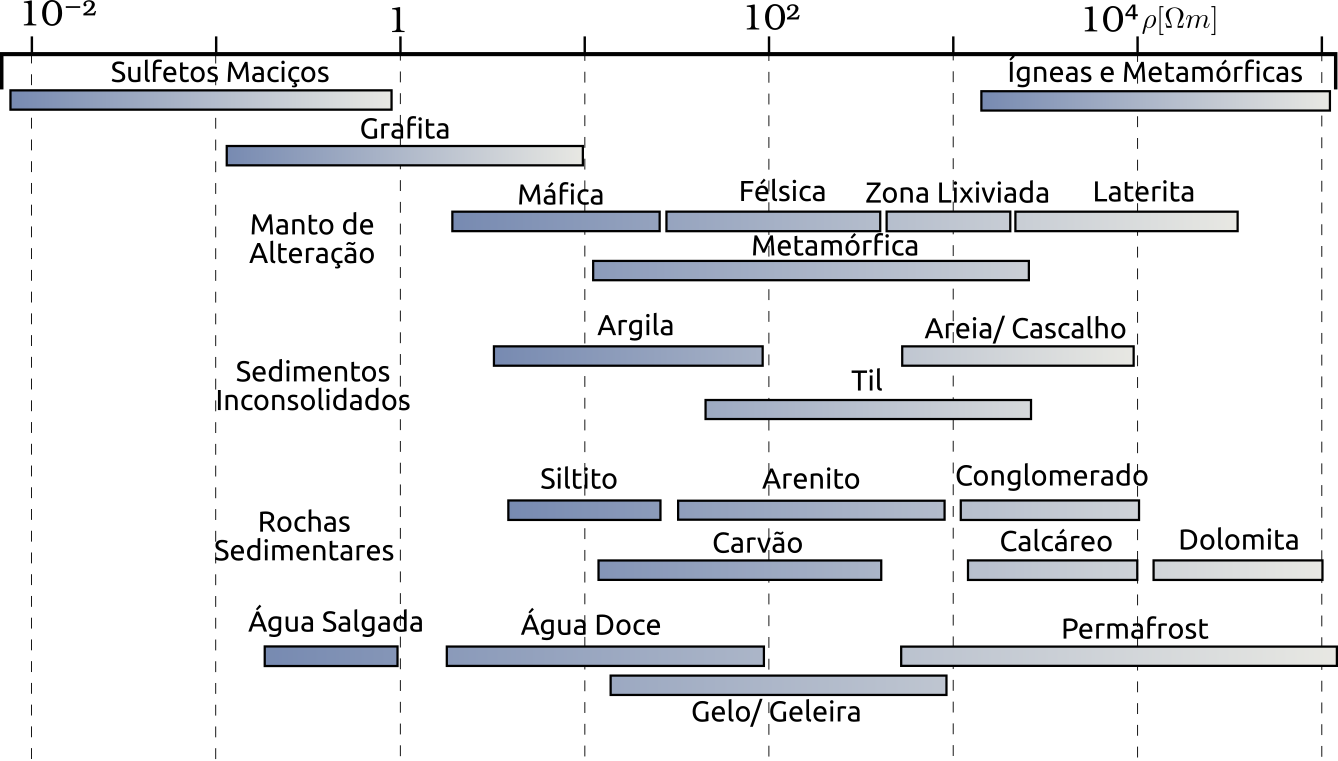
\includegraphics[width=13cm]{texto/figura/resistividade_tabela.png}
                \end{center}
            \legend{\Fonte{Adaptado \cite{palacky}.}}
            \label{tabela-resis}
        \end{figure}
    
    \section{Origem das Correntes Telúricas}
    
        O método MT utiliza-se de um amplo espectro do campo eletromagnético natural terrestre (10\textsuperscript{-4} a 10\textsuperscript{4} $Hz$) para as sondagens geofísicas. Essa característica permite que  a sondagem magnetotelúrica alcance centenas de quilômetros.
        
        O sinal MT tem sua origem nas ressonâncias de Schumann, nas micropulsações e nas variações diurnas \cite{padua2004estudos}. A figura \ref{sinalmt} mostra a contribuição de cada mecânismo no espectro MT.
        
        \begin{figure}[H]
            \caption{Campo magnético natural e as contribuições das fontes do sinal MT.}
                \begin{center}
                    \includegraphics[width=12cm]{texto/figura/padua04.eps}
                \end{center}
            \legend{\Fonte{\cite{padua2004estudos}.}}
            \label{sinalmt}
        \end{figure}
        
        As ressonâncias de Schumann tem sua origem principalmente nas tempestades equatoriais contribuindo para a fonte do sinal MT acima de 1 $Hz$, as frequências a baixo desse valor, tem origem na interação do vento solar com a magnetosfera, que geram ressonâncias Terra-ionosfera. A contribuição de parte do espectro MT, tambem pode ser explicada pela distorção do formato do campo magnético terrestre causada pelo Sol durante o dia, esse processo é chamado de variação diurna e contribui com a faixa de frequência de 10\textsuperscript{-5} a 10\textsuperscript{-4} $Hz$. 
        
        
        %\subsection{Ressonâncias de Schumann}
        
        %\subsection{Micropulsações}
        
        %\subsection{Variações Diurnas}   
        
    \section{Resposta do Método Magnetotelúrico}

        O \mt{} assim como outros métodos geofísicos eletromagnéticos, fundamentam-se nas Leis de Maxwell [\ref{lei-max-rotE} -- \ref{lei-max-divD}], pode-se partir das equações estimar os parâmetros físicos para a investigação MT, assim:
        
        \begin{equation}
            \label{lei-max-rotE}
            \rot{E} = - \devpart{\vetor{B}}
        \end{equation}
        \begin{equation}
            \label{lei-max-rotH}
            \rot{H} = \vetor{J} + \devpart{\vetor{D}}
        \end{equation}

        \begin{equation}
            \label{lei-max-divB}
            \nabla \cdot \vetor{B} = 0 
        \end{equation}

        \begin{equation}
            \label{lei-max-divD}
            \nabla \cdot \vetor{D} = \varrho                
        \end{equation}
        
        \noindent Onde,
            
        {\footnotesize \noindent
            \begin{table}[H]
                \begin{tabular*}{1cm}{p{0.05cm}p{0.1cm}p{10cm}}
                    {\footnotesize $\vec{\textrm{E}}$}  & {\footnotesize $\rightarrow$} & {\footnotesize Campo Elétrico [$V/m$] }\\
                    {\footnotesize $\vec{\textrm{B}}$}  & {\footnotesize $\rightarrow$} & {\footnotesize Campo Magnético [$T$] }\\
                    {\footnotesize $\vec{\textrm{H}}$}  & {\footnotesize $\rightarrow$} & {\footnotesize Campo Magnetizante [$A/m$]} \\
                    {\footnotesize $\vec{\textrm{J}}$}  & {\footnotesize $\rightarrow$} & {\footnotesize Densidade de Corrente [$A/m^2$]} \\
                    {\footnotesize $\vec{\textrm{D}}$}  & {\footnotesize $\rightarrow$} & {\footnotesize Campo de Deslocamento Elétrico [$C/m^2$]} \\
                    {\footnotesize $\varrho$}           & {\footnotesize $\rightarrow$} & {\footnotesize Densidade de Carga [$C/m^3$]} \\
                    {\footnotesize $t$ }                & {\footnotesize $\rightarrow$} & {\footnotesize Tempo [$s$]}
                \end{tabular*}
            \end{table}}

        Para os estudos \mt s são feitas as seguintes afirmações, que auxiliam e simplificam o desenvolvimento:
       
        \begin{quote}
            A Terra comporta-se como um condutor ôhmico e um semi-espaço isotrópico.
        \end{quote}
        
        Podemos utilizar, partindo dessas característica e atrelado a um campo eletromagnético pouco intenso as seguintes relações constitutivas:
        \begin{equation}
         \vetor{B} = \mu \vetor{H}
        \end{equation}
        
        \begin{equation}
         \vetor{D} = \varepsilon \vetor{E}
        \end{equation}
        
        \begin{equation}
         \vetor{J} = \sigma \vetor{E}
        \end{equation}

        {\footnotesize \noindent
            \begin{table}[H]
                \begin{tabular*}{1cm}{p{0.05cm}p{0.1cm}p{10cm}}
                    {\footnotesize $\mu$}          & {\footnotesize $\rightarrow$} & {\footnotesize Permeabilidade Magnética [$H/m$] }\\
                    {\footnotesize $\varepsilon$}  & {\footnotesize $\rightarrow$} & {\footnotesize Permissividade Elétrica [$F/m$] }\\
                    {\footnotesize $\sigma$}       & {\footnotesize $\rightarrow$} & {\footnotesize Condutividade Elétrica [$S/m$]} \\
                \end{tabular*}
            \end{table}}

        \noindent Cada coeficiente das relações constitutivas funcionam como tensores, variantes no tempo, para meios anisotrópicos. Para o estudo abordado e seguindo a afirmação, onde a Terra torna-se um meio isotrópico, isso implica que os tensores, $\mu$ e $\varepsilon$ são estáticos e assumem os seguintes valores:
        
        \begin{quote}
            \begin{enumerate}
                \item[$\mu$] $=$ \basedez{1{,}2566}{-6}$H/m$
                \item[$\varepsilon$] $=$ \basedez{8{,}85}{-12}$F/m$
            \end{enumerate}
        \end{quote}
        
        Utilizando as equações constitutivas podemos reescrever as equações \ref{lei-max-rotE} e \ref{lei-max-rotH}:
        
        {\setlength\arraycolsep{2pt}
        \begin{eqnarray}
            \label{rotEconstH}
            \rot{E} &=& - \devpart{\vetor{B}}; \qquad \vetor{B} = \mu \vetor{H} \nonumber \\
            \rot{E} &=& - \mu \devpart{\vetor{H}}
        \end{eqnarray}}

        {\setlength\arraycolsep{2pt}
        \begin{eqnarray}
            \label{rotHconstE}
            \rot{H} &=& \vetor{J} + \devpart{\vetor{D}}; \qquad \vetor{J} = \sigma \vetor{E} \quad \textrm{e} \quad \vetor{D} = \varepsilon \vetor{E}\nonumber \\
            & &\rot{H} =  \sigma \vetor{E} + \varepsilon \devpart{\vetor{E}}
        \end{eqnarray}}
        
        Na faixa da sondagem MT a Terra comporta-se como um condutor ôhmico, isso implica que o meio não possuem cargas livres, logo $\varrho \simeq 0$. 
        
        Para os campos pode ser assumida uma dependência temporal harmônica dada por $e^{- \imath \omega t}$, que pode ser decomposta em vários harmônicos pela transformada de Fourier, onde $t$ é o tempo e $\omega$ a frequência angular. 
    
        Portando as equações: \ref{rotEconstH}, \ref{rotHconstE}, \ref{lei-max-divB} e \ref{lei-max-divD}, podem ser reescritas como:
        
        \begin{equation}
            \label{rotEconstHreescrito}
            \rot{E} = \imath \omega \mu \vetor{H}           
        \end{equation}
        
        \begin{equation}
            \label{rotHconstEreescrito}
            \rot{H} = (\imath \omega \varepsilon + \sigma) \vetor{E}
        \end{equation}
        
        \begin{equation}
            \nabla \cdot \vetor{H}  = 0
        \end{equation}

        \begin{equation}
            \nabla \cdot \vetor{E} = 0
        \end{equation}

        Aplicando o rotacional na equação \ref{rotHconstEreescrito}, obtemos:
         
        \begin{equation}
            \label{rotrotH}
            \nabla \times \nabla \times \vetor{H} = (\imath \omega \varepsilon + \sigma) \rot{E}
        \end{equation}

        Comparando a equação \ref{rotrotH} com a equação \ref{rotEconstHreescrito}, pode-se reescreve-la como:
        
        {\setlength\arraycolsep{2pt}
        \begin{eqnarray}
            \label{preHk}
            \nabla \times \nabla \times \vetor{H} &=& (\imath \omega \varepsilon + \sigma) \rot{E}; \qquad \rot{E} = \imath \omega \mu \vetor{H} \nonumber \\
            & &\nabla \times \nabla \times \vetor{H} = \imath \omega \mu (\imath \omega \varepsilon + \sigma) \vetor{H}            
        \end{eqnarray}}
        
        Pode-se expressar a equação \ref{preHk} usando a seguinte identidade vetorial:
        
        \begin{equation}
            \nabla \times \nabla \times \vetor{A} = \nabla \nabla \cdot \vetor{A} - \nabla^2 \vetor{A} 
        \end{equation}

        \noindent Portanto:
        
        {\setlength\arraycolsep{2pt}
        \begin{eqnarray}
            \label{difH}
            \nabla \nabla \cdot \vetor{H} - \nabla^2 \vetor{H} & = & \imath \omega \mu (\imath \omega \varepsilon + \sigma) \vetor{H} \nonumber \\
            \nabla (\nabla \cdot \vetor{H}) - \nabla^2 \vetor{H} & = & \vetor{H}[\cancelto{\kappa^2}{\imath \omega \mu (\imath \omega \varepsilon + \sigma)}] \nonumber \\
            \nabla (\cancelto{0}{\nabla \cdot \vetor{H}}) - \nabla^2 \vetor{H} & = & \kappa^2 \vetor{H} \nonumber \\
            \nabla^2 \vetor{H} + \kappa^2 \vetor{H} & = &  0; \qquad \kappa^2 = \imath \omega \mu (\imath \omega \varepsilon + \sigma)
        \end{eqnarray}}        
        
        Considerando um condutor ôhmico ($\sigma \gg \omega \varepsilon$), assim:
        \begin{equation}
            \label{kappaquad}
            \kappa^2 = \imath \omega \mu \sigma
        \end{equation}
        
        \noindent Onde, $\kappa^2$ é o módulo do vetor de onda ($\vetor{k}$).
        
        A equação \ref{kappaquad} pode ser expressa seguindo a definição, como:
        
        {\setlength\arraycolsep{2pt}
        \begin{eqnarray}
            \kappa & = & \sqrt{\imath \omega \mu \sigma}; \quad \imath = e^{\imath \frac{\pi}{2}} \nonumber \\
            \kappa & = & \sqrt{\omega \mu \sigma} \sqrt{e^{\imath \frac{\pi}{2}}} \nonumber \\
            \kappa & = & \sqrt{\omega \mu \sigma} e^{\imath \frac{\pi}{4}}; \quad e^{\imath \frac{\pi}{4}} = \sqrt{1/2} (1 + \imath) \nonumber \\
            \kappa & = & \sqrt{\dfrac{\omega \mu \sigma}{2}} (1 + \imath) \nonumber \\
            \kappa & = & \dfrac{(1 + \imath)}{\delta}
        \end{eqnarray}} 
        
        \noindent Onde,
        
        \begin{equation}
            \label{shin-depth}
            \delta_\omega = \sqrt{\dfrac{2 \rho}{\omega \mu}} \longrightarrow \delta_f \approx 500  \sqrt{\frac{\rho_a}{f}}
        \end{equation}
        
        A equação \ref{shin-depth} é chamada de \en{skin-depth}\footnote{Espessura pelicular}, ela representa a profundidade de penetração da onda eletromagnética em um meio condutor.
        A partir da equação são mapeadas as litologias em subsuperfície. Porém a resistividade ($\rho$) representa todo o pacote de rochas em subsuperfície, portanto, adota-se o termo resistividade aparente ($\rho_a$) para a mesma. A resistividade efetiva ($\rho$) pode ser obtida a partir do processo de inversão geofísica.        

        O meio geológico influência diretamente a profundidade de investigação, a figura \ref{fig-skin-depth} mostra que para uma mesma frequência, ela pode representar valores diferentes de profundidade, variando o meio em subsuperfície, isso é representado por $\rho$. Os meios mais resistivos geram profundidade maiores, já meios condutivos diminuem a profundidade. Esse fenômeno é importante por que, ao interpretar as seções lito-geofísicas, é comum estudar contextos de bacias sedimentares (meio condutivo) em contado com contextos cristalinos (meio resistivo), a atenção deve-se voltar para o fato de que um mesmo período em função de $\rho$ pode representar duas profundidades diferentes, estando a estação em cima do contexto sedimentar ou em cima do contexto cristalino. 
        
        \begin{figure}[H]
            \caption[Gráfico do \en{skin-depth}]{Gráfico do \en{skin-depth} em função da frequência [$Hz$], variando a resistividade do meio}
            \begin{center}
                \includegraphics[width=12cm]{texto/figura/skin-depth.png}
            \end{center}
            \legend{\Fonte{\oautor.}}
            \label{fig-skin-depth}
        \end{figure}
        
    \section{Impedância Eletromagnética}
        
        Baseado na fundamentação teórica apresentada a seção anterior, o MT busca obter a resistividade aparente em função da profundidade. 
        
        A solução da equação \ref{difH} e da sua análoga para o campo $\vetor{E}$ são dadas por:
        
        \begin{equation}
            \label{soluH}
            \vetor{H}_{(\vetor{r})} = \vetor{H} e^{-\vetor{k} \cdot \vetor{r}}
        \end{equation}

        \begin{equation}
            \label{soluE}
            \vetor{E}_{(\vetor{r})} = \vetor{E} e^{-\vetor{k} \cdot \vetor{r}}
        \end{equation}

        %\noindent Onde $\vetor{k}$ é o vetor de onda, cujo o módulo é definido por $\kappa$ na equação \ref{kappaquad}.
        
        Substituindo a equação \ref{soluH} e \ref{soluE} em \ref{rotHconstEreescrito}, temos:
        
        {\setlength\arraycolsep{2pt}
        \begin{eqnarray}
            \label{HEpossolu}
            \nabla \times \vetor{H}e^{-\vetor{k} \cdot \vetor{r}} & = & (\imath \omega \varepsilon + \sigma) \vetor{E}e^{-\vetor{k} \cdot \vetor{r}}; \quad \sigma \gg \imath \omega \varepsilon \ \nonumber \\
            \nabla \times \vetor{H}e^{-\vetor{k} \cdot \vetor{r}} & = & \sigma \vetor{E}e^{-\vetor{k} \cdot \vetor{r}}; \quad \sigma = \dfrac{\kappa^2}{\imath \omega \mu} \nonumber \\
            \nabla \times \vetor{H}e^{-\vetor{k} \cdot \vetor{r}} & = &\dfrac{\kappa^2}{\imath \omega \mu} \vetor{E}e^{-\vetor{k} \cdot \vetor{r}}
        \end{eqnarray}} 
        
        \noindent Usando as identidades:
        
        \begin{equation}
            \nabla (e^{-\vetor{k} \cdot \vetor{r}}) = - e^{-\vetor{k} \cdot \vetor{r}} \vetor{k}
        \end{equation}

        \begin{equation}
            \nabla \times \vetor{C}(f_{(\vetor{r})}) = - \vetor{C} \times \nabla f_{(\vetor{r})} 
        \end{equation}
        
        Pode-se reescrever a equação \ref{HEpossolu}:
        
        {\setlength\arraycolsep{2pt}
        \begin{eqnarray}
            \label{EZHvetor}
            - \vetor{H} \times (- e^{-\vetor{k} \cdot \vetor{r}} \vetor{k}) = \dfrac{\kappa^2}{\imath \omega \mu} \vetor{E}e^{-\vetor{k} \cdot \vetor{r}} \nonumber \\
            \cancelto{}{e^{-\vetor{k} \cdot \vetor{r}}} (\vetor{H} \times \vetor{k}) = \cancelto{}{e^{-\vetor{k} \cdot \vetor{r}}} \dfrac{\kappa^2}{\imath \omega \mu} \vetor{E}\nonumber \\
            \vetor{E} = \dfrac{\imath \omega \mu}{\kappa^2} \vetor{H} \times \vetor{k} \nonumber \\
            \vetor{E} = \dfrac{\imath \omega \mu}{\kappa} \vetor{H} \times \dfrac{\vetor{k}}{\kappa}
        \end{eqnarray}} 
        
        \noindent A relação $\vetor{k}/\kappa$ é o versor de $\vetor{k}$ ou  $\hat{\unitario{k}}$, representando a ortogonalidade entre $\vetor{H}$ e $\vetor{E}$.
        
        A partir da equação anterior pode ser definido que $Z = \imath \omega \mu / \kappa$, esta definição é conhecida como impedância intrínseca do meio ou impedância eletromagnética, também pode ser representada da seguinte forma:
        
        \begin{equation}
            Z = \dfrac{|\vetor{E}|}{|\vetor{H}|} = \dfrac{\imath \omega \mu}{\kappa} = \sqrt{\omega \mu \rho} e^{\imath \frac{\pi}{4}}
        \end{equation}
        
        A impedância eletromagnética ($Z$) pode ser decomposta em função das componentes de $\vetor{E}$ e $\vetor{H}$, representada na forma matricial:
        
        \begin{equation}
            \label{tensor-impe}
            \left (\begin{array}{c}
                \textrm{E}_x\\
                \textrm{E}_y
                    \end{array}\right)
                =
            \left (\begin{array}{cc}
                \textrm{Z}_{xx} & \textrm{Z}_{xy}\\
                \textrm{Z}_{yx} & \textrm{Z}_{yy}
                    \end{array}\right)
            \left (\begin{array}{c}
                \textrm{H}_x\\
                \textrm{H}_y
                    \end{array}\right)
	    \end{equation}
	    
	    O método MT, então, obtém a resistividade aparente a partir da impedância eletromagnética, e atribui a ela uma profundidade, onde pode ser definida pela função de \en{skin-depth} (equação \ref{shin-depth}).          

\chapter{AQUISIÇÃO DE DADOS E DEPENDÊNCIAS}
    
    Neste capítulo será discutido como é realizada a aquisição de dados MT, e quais as técnicas atualmente utilizadas para o processamento de dados. Também será mostrado quais as dependências que foram necessárias para a construção do \software, dentre elas estão: Kivy, EMTF (Dnff e TranMT) e conversores de dados.
        
    \section{Aquisição de Dados MT}        
    
        A aquisição de dados MT consiste na obtenção dos campos elétricos ($\campo{E}_x$ e $\campo{E}_y$) e magnéticos ($\campo{H}_x$, $\campo{H}_y$ e $\campo{H}_z$), onde são os parâmetros essenciais para o cálculo da impedância ($Z$).
        
        Devido a sensibilidade do sinal das sondagens MT, os sensores devem proporcionar uma alta relação sinal/ruído e alta capacidade de ampliar o sinal medido.
        
        O arranjo amplamente adota para aquisição, são três magnetômetros distribuídos cada um paralelo a um eixo cartesiano, responsáveis pelos campos magnéticos. Para os campos elétricos, são distribuídos dois arranjos de eletrodos não polarizados, onde são acoplados horizontalmente, no sentido $x$ e $y$. A figura \ref{fig-arranjo-mt} mostra a disposição dos sensores na superfícies.
        
        Vale ressaltar que o eixo $x$ da composição cartesiana deve estar paralelo a direção do fluxo magnético terrestre, ou seja, direcionado ao polo geomagnético terrestre\footnote{Ponto na superfícies terrestre, onde, a inclinação magnética do modelo matemático para o campo magnético é $+90^\circ$}. 
        
        \begin{figure}[H]
            \caption{Arranjo para Aquisição de dados MT.}
                \begin{center}
                    \includegraphics[width=12cm]{texto/figura/arranjo-mt.eps}
                \end{center}
            \legend{\Fonte{\oautor.}}
            \label{fig-arranjo-mt}
        \end{figure}
        
        Os sensores registram a variação da amplitude do sinal em função do tempo, esses registros são chamados de series temporais e são considerados os dados brutos do método. 
        
        Devido ao grande intervalo do espectro eletromagnético que abrange as sondagens MT ($10^{-3}\, Hz$ a $10^{4}\, Hz$), são configuradas varias taxas de aquisições diferentes. Para cada escolha de taxa de aquisição é considerada a representatividade do sinal respeitando a frequência de Nyquist \cite{nyquist28}. A representatividade é muito importante, pois, o sinal medido pelos sensores é a composição de várias ondas com frequências angulares diferentes, se a taxa de aquisição for menor que duas vezes a frequência da onda, ela não pode ser representada fielmente.  
        
        A figura \ref{fig-aquisicao} exemplifica o conceito apresentado no paragrafo anterior, no exemplo é mostrado a composição de um onda com 10 frequências diferentes ($f_{\omega(t)}$), variando de $1$ a $10\, Hz$, se atribuirmos à ela uma taxa de aquisição de $10\,Hz$ pode-se perceber que a frequência de $6\,Hz$ não é representada corretamento, já percebe-se que para a frequência de $1\,Hz$ é super representada, isso acaba aumentando o tamanho dos arquivos de aquisição. A escolha da taxa de aquisição deve conciliar na melhor forma possível esses dois fatos.
        
        \begin{figure}[H]
            \caption{Aquisição de Dados Discretos.}
                \begin{center}
                    \includegraphics[width=13cm]{texto/figura/fourier2.eps}
                \end{center}
            \legend{\Fonte{\oautor.}}
            \label{fig-aquisicao}
        \end{figure}
    
        As taxas de aquisições comumente utilizadas são valores estimados por potências de 2, isso facilita na decomposição das frequências pela transforma de Fourier. Cada taxa de aquisição é chamada de \en{Banda} e varia de nome para cada equipamento utilizado. 
    
    \section{Processamento de Dados MT}
        Tradicionalmente o grande processamento de dados geofísicos é chamado de inversão, onde esse tenta ajustar um modelo físico que melhor represente o conjunto de dados. Porém para dados MT faz-se necessário antes das técnicas de inversão, o pré-processamento.
        
        O pré-processamento consiste, sucintamente, em realizar processamentos de filtragem, tratamentos estatísticos, conversão de dados, mudança de domínios e mesclagem de arquivos.
    
        A primeira etapa do pré-processamento é a conversão dos arquivos de binários para ASCII, esse processo é opcional, porem como boa prática é realizado para melhorar a legibilidade por parte dos usuários sobre os dados.
        
        Após a conversão são realizados técnicas de filtragem, a mudança do domínio dos dados de tempo para frequência angular, e calculo do tensor impedância ($Z$), esse processo será demonstrado mais detalhadamente no seção \ref{sec-robusto}, a técnica adotada para esse processo é chamado de processamento robusto, EMTF \cite{robusto-egbert}, atualmente é a técnica mais confiável e amplamente utilizadas no meio acadêmico para manipulação dos dados.
        
        Como comentado na seção anterior, devido as limitações dos equipamentos, os dados são coletados separadamente para cada banda. Cada banda após o processamento robusto gera um arquivo com extensão \en{.zss}, nesses arquivos são armazenados os tensores de impedância, ou seja, cada componente da matriz $Z$, para cada período.
        
        A etapa seguinte do processamento consiste em escolher, dentro de todos arquivos, a melhor composição dos períodos para todo o espectro de estudo, esse processo é minucioso e depende da experiencia do usuário. Nessa etapa deve-se plotar cada arquivo e verificar a sua coerência dentro do conjunto total dos dados.
        
        A última etapa do pré-processamento é mesclar os períodos escolhidos em um único arquivo, esses arquivos contem todas as informações necessárias para realizar os processos de inversão.
        
        A figura \ref{fluxo-preprocessamento} ilustra as etapas de pré-processamento.
        
        \begin{figure}[H]
            \caption{Fluxograma de Pré-processamento.}
                \begin{center}
                    \includegraphics[width=15cm]{texto/figura/fluxo_preprocessamento.eps}
                \end{center}
            \legend{\Fonte{\oautor.}}
            \label{fluxo-preprocessamento}
        \end{figure}
        
    \section{Formatos de Arquivos de Dados MT}   
    
        Parte das funções do \software{} desenvolvido será a simplificação no processo de conversão de dados, atualmente os formatos mais utilizados, são:
        
        {\footnotesize \noindent
            \begin{table}[H]
                \begin{tabular*}{1cm}{p{2.05cm}p{0.5cm}p{10cm}}
                    \en{TS-format}       & {\footnotesize $\rightarrow$} & \en{Time Series Format (.ats)} \\
                    \en{Z-file}          & {\footnotesize $\rightarrow$} & \en{Z (Impedance Tensor) File (.zss)} \\
                    \en{J-format}        & {\footnotesize $\rightarrow$} & \en{Jones Format (.dat)} \\
                    %\en{EDI-format}      & {\footnotesize $\rightarrow$} & \en{Eletrical Data Interchange Format (.edi)} \\
                \end{tabular*}
            \end{table}}
        
        Os arquivos \en{TS} são utilizados para registrar as series temporais, onde são armazenadas as amplitudes registradas pelos sensores em função do tempo. A grande parte dos equipamentos tem como saída padrão a forma binária dos arquivos \en{TS}. Os arquivos binários podem  posteriormente serem convertidos para o formato ASCII.
        
        O arquivo \en{TS} é composto por dois blocos, o primeiro é destinado a comentários e configurações da aquisição, já  o segundo compõe o bloco de dados, distribuídos em cinco colunas, cada uma registra a amplitude do sinal dos sensores $H_x$, $H_y$, $H_z$, $E_x$ e $E_y$. O tempo associado a cada registro pode ser estimado pela hora de inicio e a taxa de aquisição da rodada.   
        
        Exemplo de arquivo \en{TS} (ASCII):

        \begin{footnotesize}        
\begin{verbatim}
        # time series file from mp2ts 
        # date: Mon May 12 10:15:57 1997
        # input file: sno101/sno101as.1mp
        # site description: KM 222.5
        # Latitude   :062:39:47 N
        # Longitude  :116:12:32 W
        # LiMS         number :           52
        # Magnetometer number :           52
        # Ex line length (m):     100.0000000
        # Ey line length (m):     100.0000000
        # Azimuths relative to: MAGNETIC NORTH 
        # Ex azimuth;          -17
        # Ey azimuth;           73 
        # Hx azimuth;          -17 
        # Hy azimuth;           73 
        1.98250   0.878400    3.64780    1.10889    2.02644                                  
        1.93980   0.976000    3.65390    1.15682    2.01610                                     
\end{verbatim}
\end{footnotesize}
            \begin{flushright}
                \cite{ts-format}
            \end{flushright}
        
        Após realizar a transformada de Fourier e o calculo do tensor impedância, não são mais necessários carregar todas as informações das series temporais, pois a partir do tensor impedância é possível estimar todos os parâmetros associados a cada período, tais como: $\rho_a$, $\phi$ e as componentes do próprio tensor: $Z_{xx}$, $Z_{xy}$, $Z_{yx}$ e $Z_{yy}$, as componentes do tensor são importantes para a interpretação da adimensionalidade dos dados.
        
        Como discutido na seção anterior a saída padrão do TranMT (programa adota para os cálculos do tensor impedância), são os arquivos \en{.zss}, esses arquivos são estruturados na forma de blocos, onde, cada bloco representa um período e nele contem o próprio tensor impedância, a matriz de covariância inversa e a matriz de covariância residual.
        
        Exemplo de arquivo \en{Z}:
        
\begin{footnotesize}        
\begin{verbatim}
      **** IMPEDANCE IN MEASUREMENT COORDINATES ****
      ********** WITH FULL ERROR COVARINCE**********
     Robust Single station                                                           
     station    :ufb104a091_03B      
     coordinate  -10.47560  -38.43750  declination   -23.00
     number of channels   5   number of frequencies   16
      orientations and tilts of each channel 
         1     0.00     0.00 ufb104a  Hx    
         2    90.00     0.00 ufb104a  Hy    
         3     0.00     0.00 ufb104a  Hz    
         4     0.00     0.00 ufb104a  Ex    
         5    90.00     0.00 ufb104a  Ey    
     period : 1.116071E-03    decimation level   1    freq. band from
     1600 to   1984
     number of data point  29853 sampling freq. 4.096000E+03 Hz
      Transfer Functions
       3.7279E-03  5.5604E-03 -1.2527E-03 -4.9609E-03
       5.7064E+01  1.7047E+01  3.1437E+02  2.1458E+02
      -2.6267E+02 -1.9591E+02 -3.2340E+01 -1.3460E+00
      Inverse Coherent Signal Power Matrix
       1.3513E+05  0.0000E+00
      -1.3265E+04  1.9036E+03  1.5955E+04  0.0000E+00
      Residual Covariance
       3.2219E-11  0.0000E+00
       6.8311E-10 -1.4571E-10  1.4028E-04  0.0000E+00
       1.2952E-10  2.3198E-10 -7.8350E-07 -1.5203E-07  1.3332E-04  0.0000E+00                                     
\end{verbatim}
\end{footnotesize}
        
        A partir dos arquivos \en{Z} (\en{.zss}), pode-se calcular a resitividade aparente ($\rho_a$) a partir da seguinte equação \cite{z-files}:
        
        \begin{equation}
         \rho_a = \dfrac{T|Z_{ij}|^2}{5}
        \end{equation}

        \noindent e para se obter a fase ($\phi$) pode-se calcular, a partir:
        \citar{não me lembro se no brasil usa-se arctan ou tan$^{-1}$}
        \begin{equation}
         \phi = \dfrac{180}{\pi} \textrm{tan}^{-1}\left [\dfrac{\Im(Z_{ij})}{\Re(Z_{ij})} \right ]
        \end{equation}

        Os erros associados a cada componente podem ser obtidos a partir das matrizes de covariância, assim como os erros para $\rho_a$ e $\phi$.
        
        Os arquivos \en{J}, análogo aos arquivos \en{Z}, armazenam as informações do tensor, porém, a estrutura é mais sintetizada. Os arquivos são estruturados em dois blocos, um destinado a configurações, tais como: localização, elevação, nome da estação e azimute. O segundo bloco é destinado aos dados \cite{j-format}.
        
        A estrutura base utilizada para os dados é composta por quatro sub-blocos, cada um representando uma componente do tensor. O sub-bloco é divido em cinco colunas, onde assumem respectivamente a seguinte ordem: 
        
\begin{footnotesize}        
\begin{verbatim}
            Zij SI units (ohms)                 < componente
            n                                   < numero de periodos
                periodo(n)  Real  Imaginario    Erro    Peso
\end{verbatim}
\end{footnotesize}
               
        Os arquivos \en{J} recebem a extensão \en{.dat}, e são os arquivos necessários para as etapas de inversão, a adoção desse formato para essa etapa, se da pela fácil leitura dos períodos e por armazenar toda a sondagem em um único arquivo, ele armazena a mesclagem de todas as diferentes janelas resultantes do processamento EMTF.
        
        Exemplo de arquivo \en{J}:
        
\begin{footnotesize}        
\begin{verbatim}
        >STATION   =bor608b
        >AZIMUTH   =    -23.0000
        >LATITUDE  =    -8.72768
        >LONGITUDE =   -37.84493
        >ELEVATION =    664.0000
        bor608b -23.0
        ZXX SI units (ohms)
        2
            1.1161e-04   -6.6462e-02   -1.0728e-01    1.7715e-03   1
            1.5625e-04    7.7005e-04   -1.0442e-01    2.9007e-03   1
        ZXY SI units (ohms)
        2
            1.1161e-04    2.5648e+00    1.2953e+00    2.5613e-03   1
            1.5625e-04    2.4467e+00    1.4059e+00    5.9294e-03   1
        ZYX SI units (ohms)
        2
            1.1161e-04   -2.3499e+00   -1.1104e+00    1.6657e-03   1
            1.5625e-04   -2.3904e+00   -1.2251e+00    3.0355e-03   1
        ZYY SI units (ohms)
        2
            1.1161e-04    7.1532e-02    3.1711e-02    2.4082e-03   1
            1.5625e-04    5.9528e-02    3.7107e-02    6.2053e-03   1
\end{verbatim}
\end{footnotesize}
    
    \section{Processamento Robusto -- EMTF}
        \label{sec-robusto}
        
            O processamento dos dados parte primeiramente da análise espectral, onde primeiro faz-se necessário a mudança do domínio do tempo para a frequência angular e em seguida a filtragem, remoção de tendências e de dados ruins.
            
            O pacote EMTF \cite{egbert-emtf} desenvolvido por Gary D. Egbert, é um conjunto de programas escrito em \en{Fortran 77} que realizam processamento tais como: mudança de domínio, cálculo do tensor impedância, plotagem e alguns tipos de conversores de dados. 
            
            A mudança do domínio do tempo para frequência angular é realizado pelo programa Dnff, contido no pacote, esse programa realiza a troca do domínio través da \en{cascade decimation} \apud{wight1980cascade}{padua2004estudos} uma alternativa ao FFT (\en{Fast Fourier Transform}\footnote{Transformada Rápida de Fourier}).
            
            Antes de efetuar a transformada de Fourier, as séries temporais são re-amostradas, essas re-amostragem são chamadas de janelas e tem o objetivo de minimizar as distorções causadas pelas reverberações da transformada de Fourier.
            
            Para estimar as componentes do tensor impedância o programa parte dos seguintes cálculos:
            
            A partir da equação \ref{tensor-impe} podemos representa-la na forma do sistema:
            
            \citar{terminar ....}
        \subsection{Função de Transferências}
           
           \cite{robusto-egbert}
           
    \section{Pacotes de Processamento do Grupo Geoma -- INPE}
    
        O grupo GEOMA do INPE (Institudo Nacional de Pesquisas Espaciais) oferece treinamentos para alunos e colaboradores. O grupo dispõe de um série de \en{scripts} e programas para auxiliar na manipulação do processamento MT.

        Os \en{scripts} oferecidos para o processamento MT foram desenvolvidos, em grande parte, pelo Dr. Marcelo Banik de Pádua e pelo Me. Marcelo Banik de Pádua.% os mesmo \en{scripts} foram obtidos sobre comunicação privada pelo autor.
        
        O programa desenvolvido faz uso dos \en{scripts} como ``ponte'' entre a interface e o os programas EMTF, como também para conversores de dados. Um exemplo é o programa \en{processamentoZ} que prepara os dados e extraí os parâmetros necessários para as rotinas Dnff e TranMT. 
        
        Para as plotagens dos gráficos é utilizado o programa GMT \cite{gmt}(figura \ref{plot-cmp-tf}). Embora o programa desenvolvido tenha a sua própria saída gráfica, foi desenvolvida uma extensão que exporta as imagens utilizando o \en{Kernel} do GMT, essa extensão visa não causar estranheza em usuários já acostumados com as imagens geradas pelo GMT.  
    
        \begin{figure}[H]
            \caption{Saída Gráfica Gerada pelo \en{script}: \en{plot-cmp-tf}, utilizando o GMT.}
                \begin{center}
                    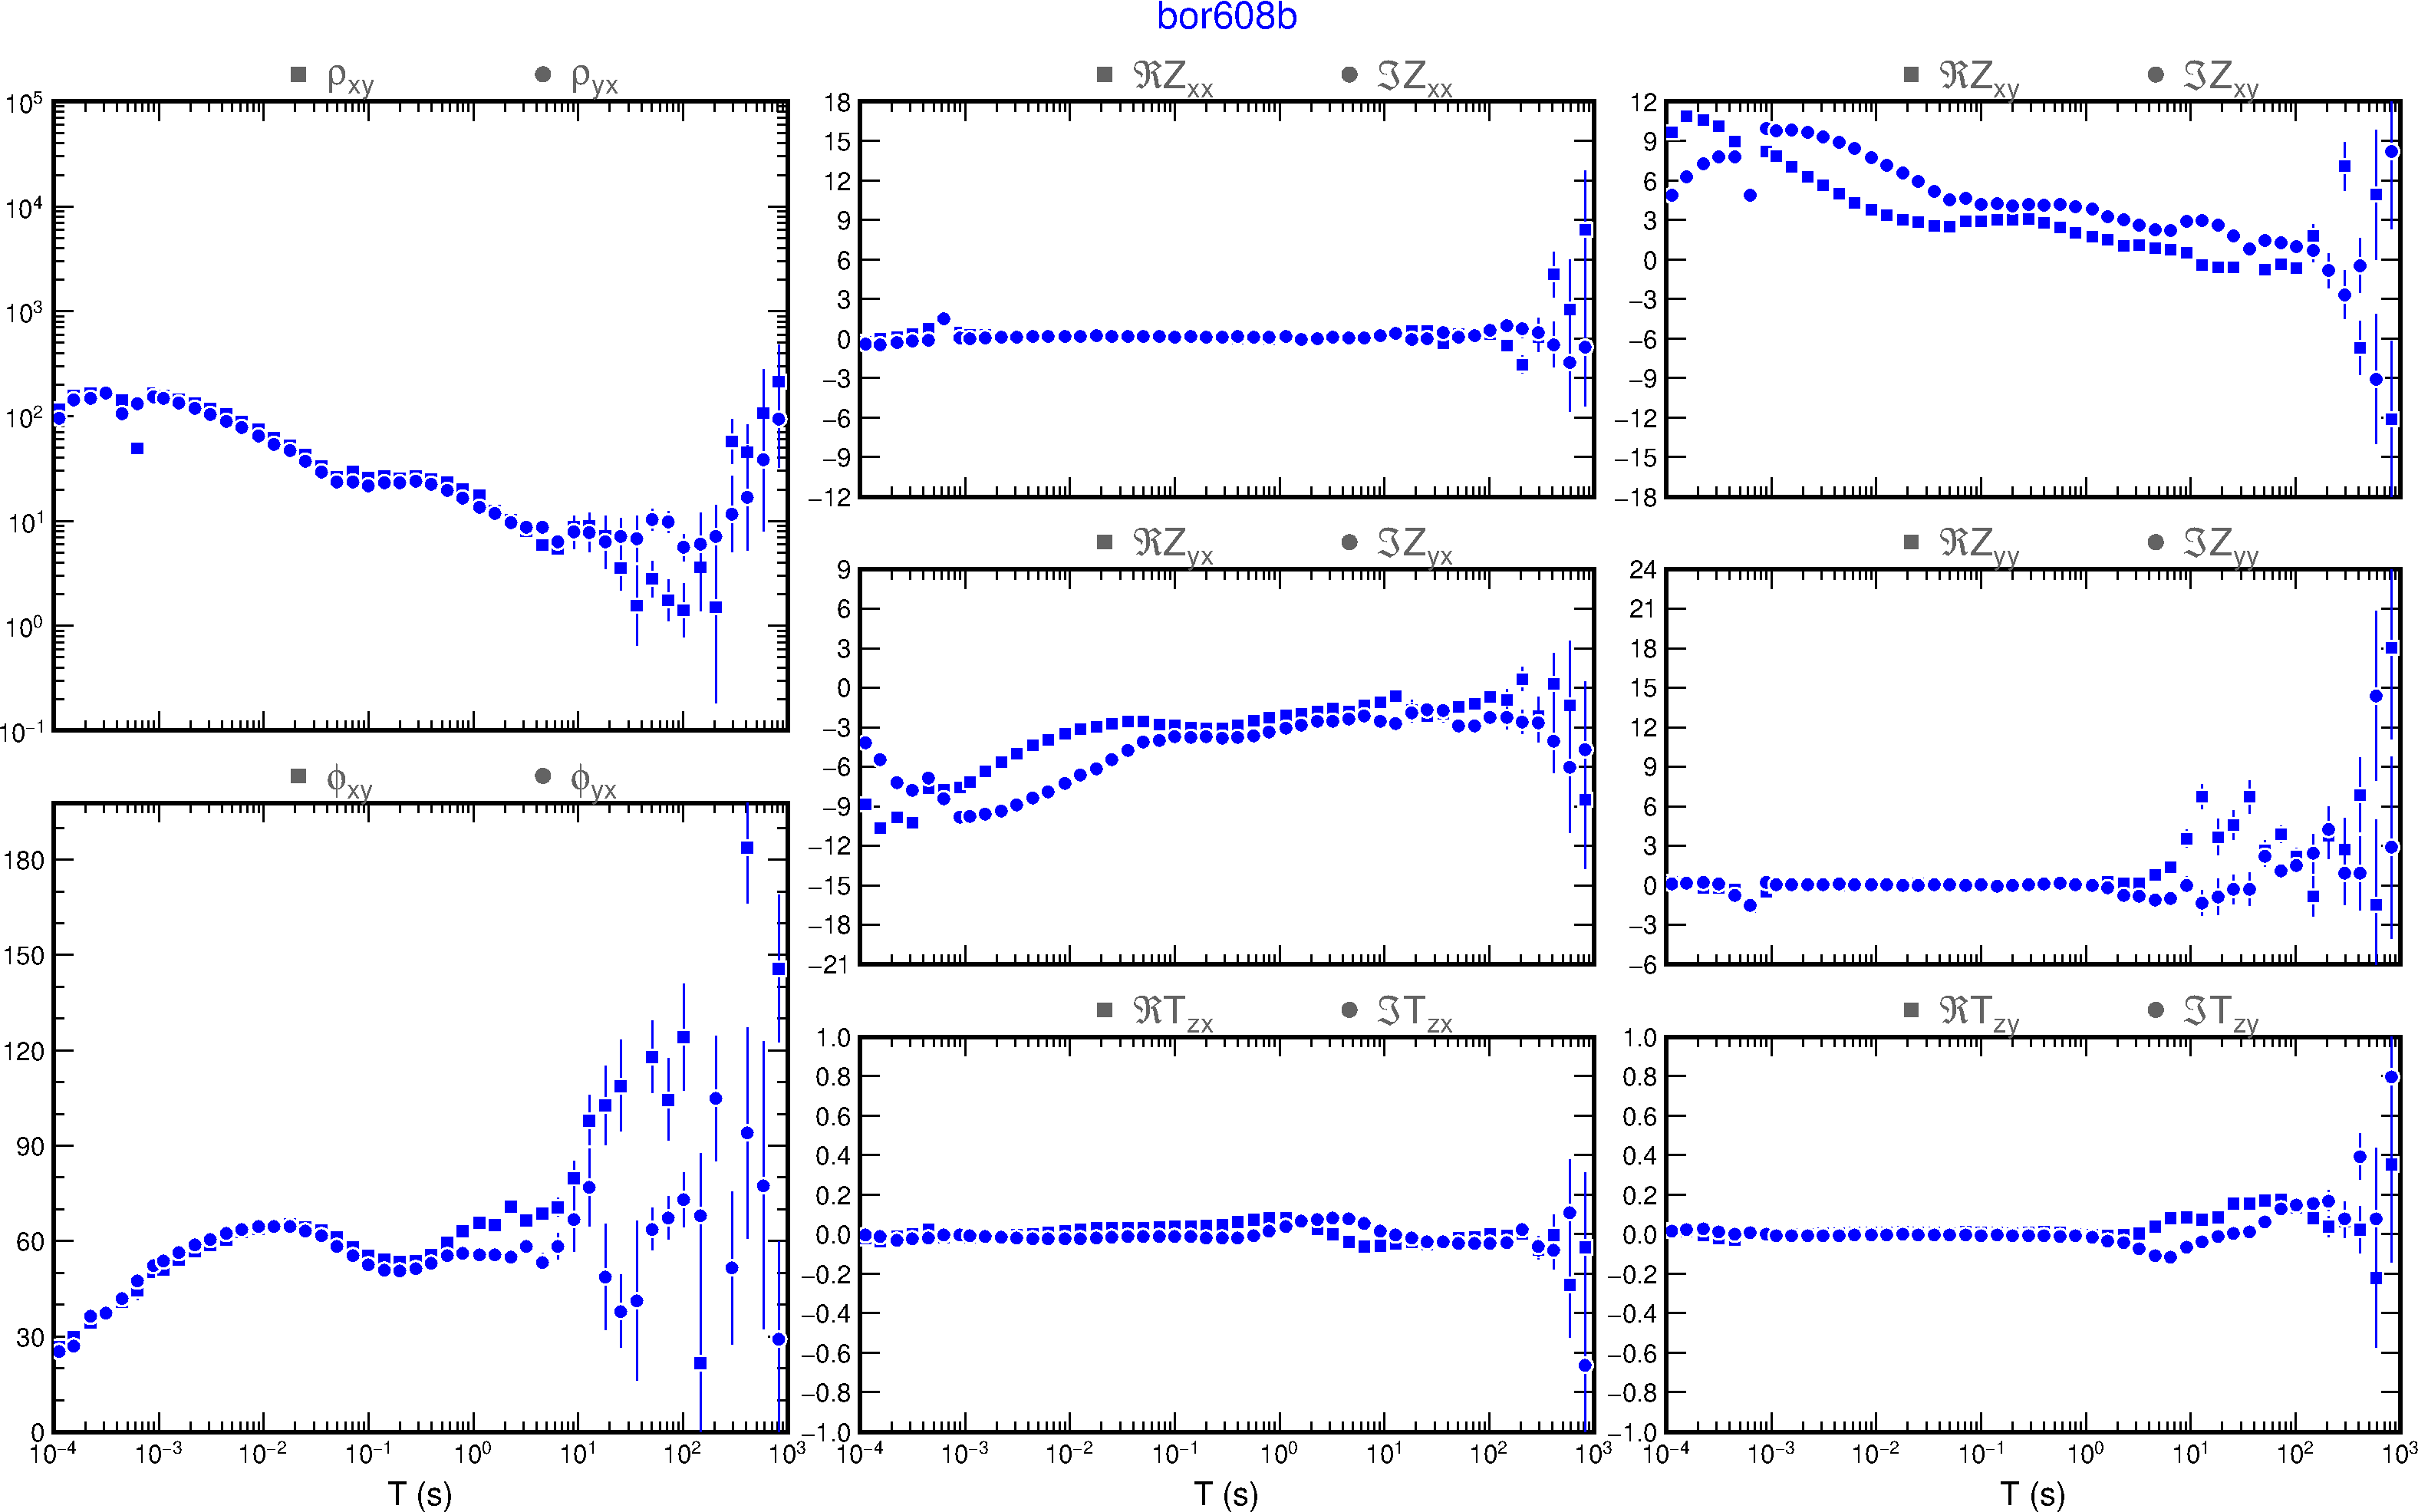
\includegraphics[width=15cm]{texto/figura/plot-cmp-tf.png}
                \end{center}
            \legend{\Fonte{\oautor.}}
            \label{plot-cmp-tf}
        \end{figure}

    
    \section{Construtor Gráfico -- Kivy}

        \citar{escrever se der tempo}
    

\chapter{DESENVOLVIMENTO E RESULTADOS DO PampaMT}

    O \en{software} desenvolvido recebeu o nome de PampaMT, em homenagem a Universidade Federal do Pampa. O desenvolvimento iniciou-se em janeiro de 2018, com o primeiro protótipo de codinome RiMT, vizando testar os conceitos e a viabilidade das funções para o programa. Em junho de 2018 o código foi reestruturado e reescrito, atentando para os problemas e adicionando novas funções baseando no protótipo. A principal mudança foi a construção do \en{software} em módulos, facilitando a adição e manutenção de novas funções.
    
    No apêndice A pode ser encontrado o caminho para o código fonte do programa, junto com as informações para a instalação. O PampaMT foi desenvolvido para ambiente Linux rodando em base Debian. O código foi escrito em \Python, com alguns trechos escritos em \Shell{} para instalação e comunicação da interface com os executáveis dos programas Dnff e TranMT.
    
    O PampaMT foi dividido em duas etapas de processamento: a primeira destinada a criação do projeto; escolha dos arquivos a serem processados e a processamento EMTF. A segunda parte foi destinada a escolha das melhores rodadas e períodos, esse processo destina a maior interação com o usuário e representa a principal justificativa para o desenvolvimento do \en{software}. 
    
    A figura \ref{tela_inicial} mostra a primeira tela ao executar o PampaMT, nela pode-se escolher criar um novo projeto ou abrir um já existente.
    
    \begin{figure}[H]
        \caption{Tela Inicial PampaMT}
            \begin{center}
                \includegraphics[width=16cm]{texto/figura/tela1_com_fluxograma.eps}
            \end{center}
        \legend{\Fonte{\oautor.}}
        \label{tela_inicial}
    \end{figure}
    
     Após a escolha do diretório para um novo projeto, o usuário é direcionado a escolha dos arquivos \en{TS}, nele o usuário pode escolher entre três equipamentos: ADU-06, ADU-07 e LiMS, a seleção pode ser automática ou adicionada cada estação individualmente (figura \ref{tela_sel_site}). 
    
    \begin{figure}[H]
        \caption{Seleção das Estações}
            \begin{center}
                \includegraphics[width=16cm]{texto/figura/tela2_com_fluxograma.eps}
            \end{center}
        \legend{\Fonte{\oautor.}}
        \label{tela_sel_site}
    \end{figure}
    
    Os dados após a seleção, são copiados para o diretório: \textbf{DADOS\_MT/projeto}, esse processo é realizado para prever eventuais perdas dos arquivos. Os dados então são convertidos e salvos no diretório: \textbf{PROC\_MT/projeto} 
    
    O usuário será levado a tela do processamento EMTF, esse processo já estabelece algumas configurações padrão, entretanto o usuário pode alterar qualquer configuração, tais como, escolher uma nova janela ou alterar o horário do relógio dos dados (figura \ref{conf-procZ}).
    
    \begin{figure}[H]
        \caption{Tela de Configuração para o EMTF}
            \begin{center}
                \includegraphics[width=16cm]{texto/figura/tela3_com_fluxograma.eps}
            \end{center}
        \legend{\Fonte{\oautor.}}
        \label{conf-procZ}
    \end{figure}
    
    O processo EMTF tende a demorar um tempo considerável, cerca de 1 a 2 minutos para cada estação, para um levantamento típico de 30 estações por perfil esse processo pode demorar de 20 a 30 minutos, visto a grande quantidade de recursos do computador que ele consome. Finalizado o processo EMTF a janela é fechada e inicia-se o tela principal do PampaMT (figura \ref{tela-prin}).
    
    \begin{figure}[H]
        \caption{Tela Principal PampaMT}
            \begin{center}
                \includegraphics[width=16cm]{texto/figura/tela4.png}
            \end{center}
        \legend{\Fonte{\oautor.}}
        \label{tela-prin}
    \end{figure}
    
    
    Na tela principal contem todas as funcionalidades do PampaMT, incluindo a etapa de criação de um novo projeto. O carácter modular do PampaMT ajuda na adição de novas funcionalidades, como por exemplo, integração por programas SIG, integração com visualizados de dados, como o GMT, dentre outros. Um exemplo notável é a adição do programa RhoplusGUI em desenvolvido pelo autor, para o projeto PIBIC/INPE/CNPq ``Desenvolvimento de Interface Gráfica Amigável para Validação de Dados Magnetotelúrico a Partir do Processamento Rho+''. Esse programa auxilia na manipulação de dados para o processamento Rho+ \cite{parker1996optimal}, onde foi necessário adicionar poucas linhas de código para inclui-lo no PampaMT (figura \ref{rhoplusGUI}).
    
    \begin{figure}[H]
        \caption{Integração com Outros Programas}
            \begin{center}
                \includegraphics[width=16cm]{texto/figura/rhoplusGUI.eps}
            \end{center}
        \legend{\Fonte{\oautor.}}
        \label{rhoplusGUI}
    \end{figure}
    
    A principal função que o usuário utilizará, será a escolha dos melhores períodos e rodadas. Esse processo vinha sendo executado, plotando cada arquivo \en{.zss} e contando manualmente a posição dos melhores períodos. Então, após a contagem, o usuário deve anotar os pontos que indicam os períodos, e finalmente executar o \en{script}: \en{ToJones}. Esse \en{script} mescla os arquivos \en{.zss} com os períodos escolhidos e converte-os para o formato \en{J} (\en{.dat}).
    
    Esse processo foi incorporado no PampaMT com a escolha dos períodos sendo realizada com o cursor. O usuário habilita a função de seleção, e o programa plota todos os pontos possíveis para a rodada escolhida, por fim o usuário arrasta uma janela de seleção e todos os períodos contidos nessa janela são selecionados (figura \ref{selc-perio}).
    
    \begin{landscape}
    \begin{figure}[h]
        \caption{Seleção dos Períodos}
            \begin{center}
                \includegraphics[width=23cm]{texto/figura/tela3_selecionando.png}
            \end{center}
        \legend{\Fonte{\oautor.}}
        \label{selc-perio}
    \end{figure}
    \end{landscape}
    
    Após escolher os melhor períodos o usuário pode executar o \en{script}: \en{ToJones}, onde esse é realizado ao pressionar o botão no canto inferior esquerdo, o PampaMT abre uma caixa de diálogo para nomear o arquivo de saída, e executa o \en{script}, finalizando a ultima etapa do pré-processamento.
    
    A utilização do PampaMT para o pré-processamento elimina completamente o uso de linhas de comando, assim o tempo de processamento e aprendizagem é diminuído drasticamente. Para efeitos de comparação, ao utilizar o programa em fase alfa, usuários que nunca tiveram contato com o terminal \Shell, puderam executar e processar os dados com sucesso.
    
    A Figura \ref{teste1} mostra o tempo que três usuários geofísicos, onde não possuem familiaridade com o terminal \en{shell}, utilizaram para concluir o pré-processamento de duas estações teste: ufb104a e ufb105a.
    
    \begin{figure}[H]
        \caption{Tempo de Processamento -- Teste Alfa}
            \begin{center}
                \includegraphics[width=13cm]{texto/figura/tempoLWM.png}
            \end{center}
        \legend{\Fonte{\oautor.}}
        \label{teste1}
    \end{figure}
    
    
    

%\chapter{RESULTADOS E APLICAÇÃO DO PAMPAMT}
    
    contaração do tempo de processamnto
    
    aprendizagem dados mt
    
    \section{Aplicação do PampaMT}
    
        \subsection{Área de Estudo}
        
        \subsection{Contexto Geológico}
        
        \subsection{Processamento dos Dados}
        
        \subsection{Resultados e Interpretação Geofísica}
        
        

\chapter{CONSIDERAÇÕES FINAIS}
    
    Rodando a versão de teste interno (versão alfa), a utilização do PampaMT para processamentos sugere que o principal fator, o tempo, foi drasticamente reduzido. O que tornou o processamento de dados magnetotelúricos mais dinâmico.
    
    A continuidade desse trabalho será ampliar o uso do PampaMT, adicionando novas funções, tais como: processos de inversão, modelagem, referência remota, dentre outros.
    
    \citar{escrever um pouco mais}


% ==============================================================================

        
% PÓS-TEXTUAL
% ==============================================================================
\postextual     % Inicia os elementos pós-textuais
% ==============================================================================


% REFERENCIAS
% ==============================================================================
\bibliography{bibliografia}         % Imprime a referencia bibliografica
% ============================================================================== 
 
 
% APÊNDICE
% ==============================================================================
\apendices                      % Inicia os apêndices

\chapter{Código Fonte PampaMT}
    
    \vspace*{1cm} 
    
    O programa PampaMT esta armazenado no servidor GitHub, atualmente o mesmo é a maior comunidade de códigos fontes, nela podemos encontrar o \en{Kernel} Linux, a plataforma SU (\en{Seismic Unix}), o pacote abn\TeX2, dentre um vasto catálogo de outros projetos.   
    
    \vspace*{1cm}
    
    \begin{center}
    Repositório com o código fonte na data de entrega do trabalho de conclusão de curso.
    \end{center}
    
    \begin{figure*}[h]
        \begin{center}
            \includegraphics[width=5cm]{texto/figura/qr-code-pampamt.eps}
        \end{center}
    \end{figure*}
    \begin{center}
        \url{https://github.com/PatrickRogger/PampaMT}
    \end{center}
    
    \begin{center}
    Repositório com o código fonte para desenvolvedores.
    \end{center}
    
    \begin{figure*}[h]
        \begin{center}
            \includegraphics[width=5cm]{texto/figura/qr-code-git-pampamt.eps}
        \end{center}
    \end{figure*}
    \begin{center}
        \url{https://github.com/PampaMT/PampaMT}
    \end{center}

    \vfill
\chapter{Pré-processamento Usando o Método Tradicional}

    %\begin{landscape}
    \begin{figure}[H]
        \caption{Manual -- bor603b}
            \begin{center}
                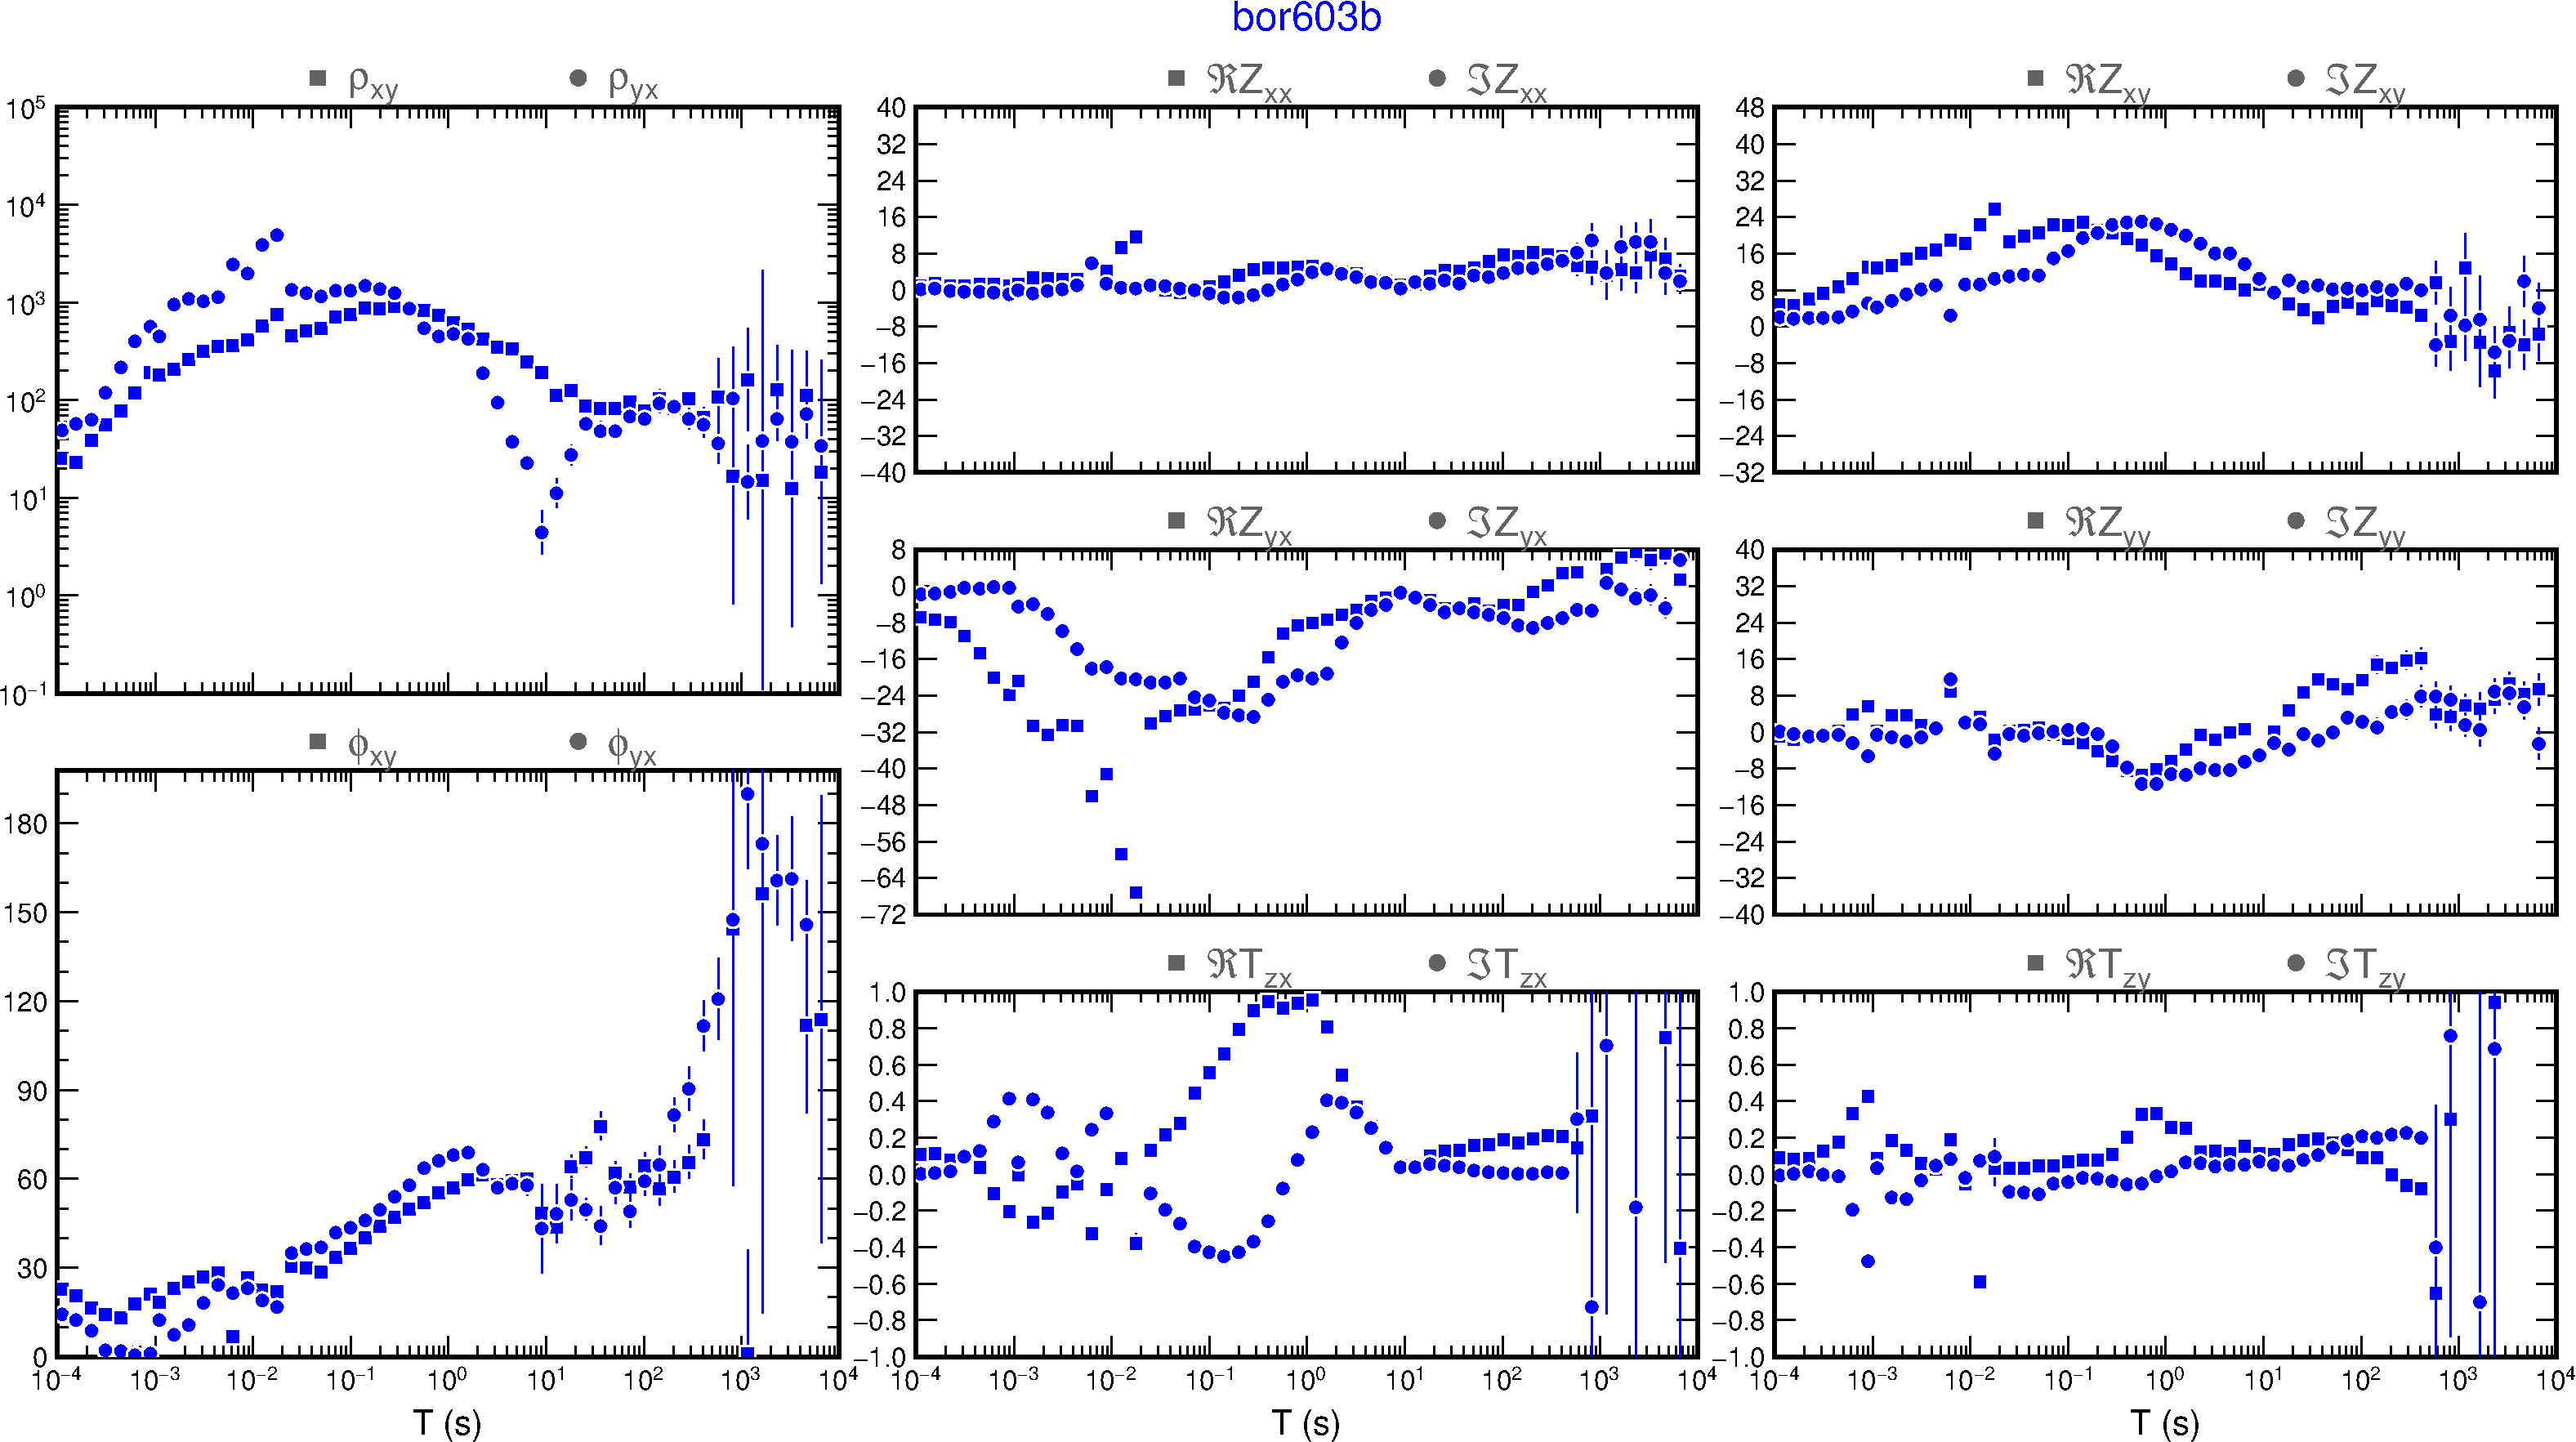
\includegraphics[width=15cm]{texto/figura/sites/M-bor603b.png}
            \end{center}
        \legend{\Fonte{\oautor.}}
    \end{figure}
    %\end{landscape}
    \begin{figure}[H]
        \caption{Manual -- bor604a}
            \begin{center}
                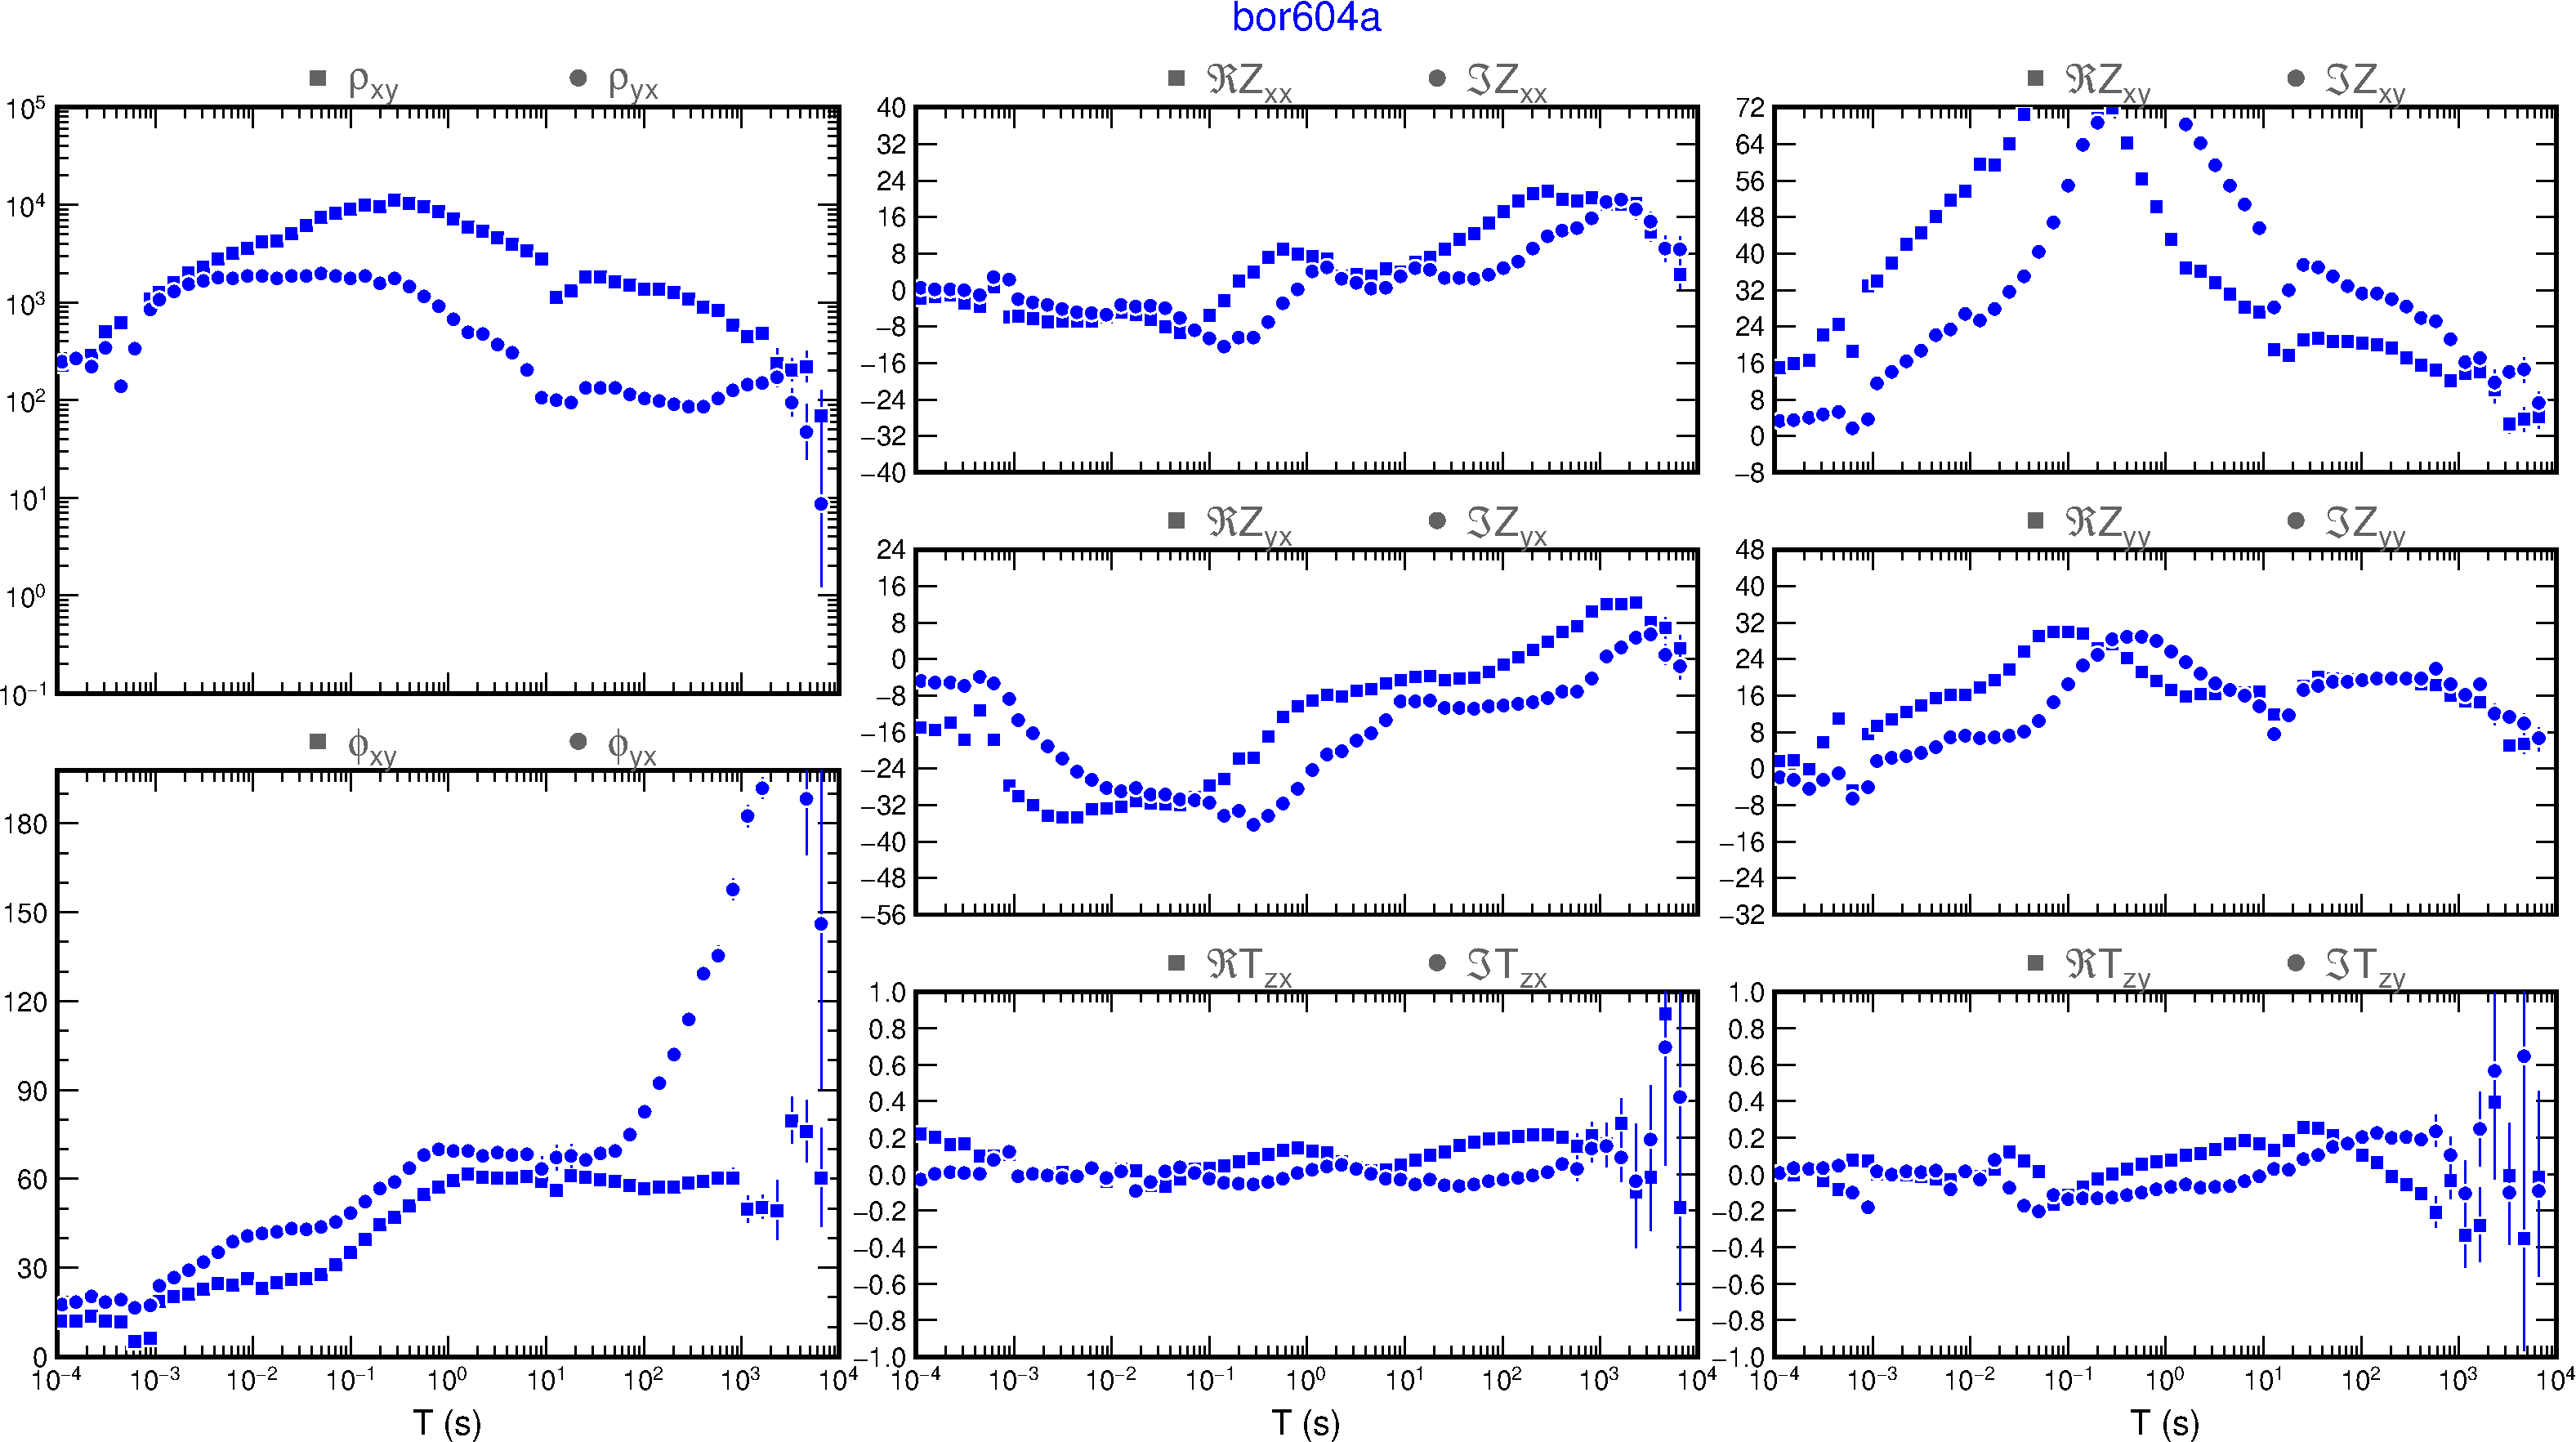
\includegraphics[width=15cm]{texto/figura/sites/M-bor604a.png}
            \end{center}
        \legend{\Fonte{\oautor.}}
    \end{figure}
    
    \begin{figure}[H]
        \caption{Manual -- bor604b}
            \begin{center}
                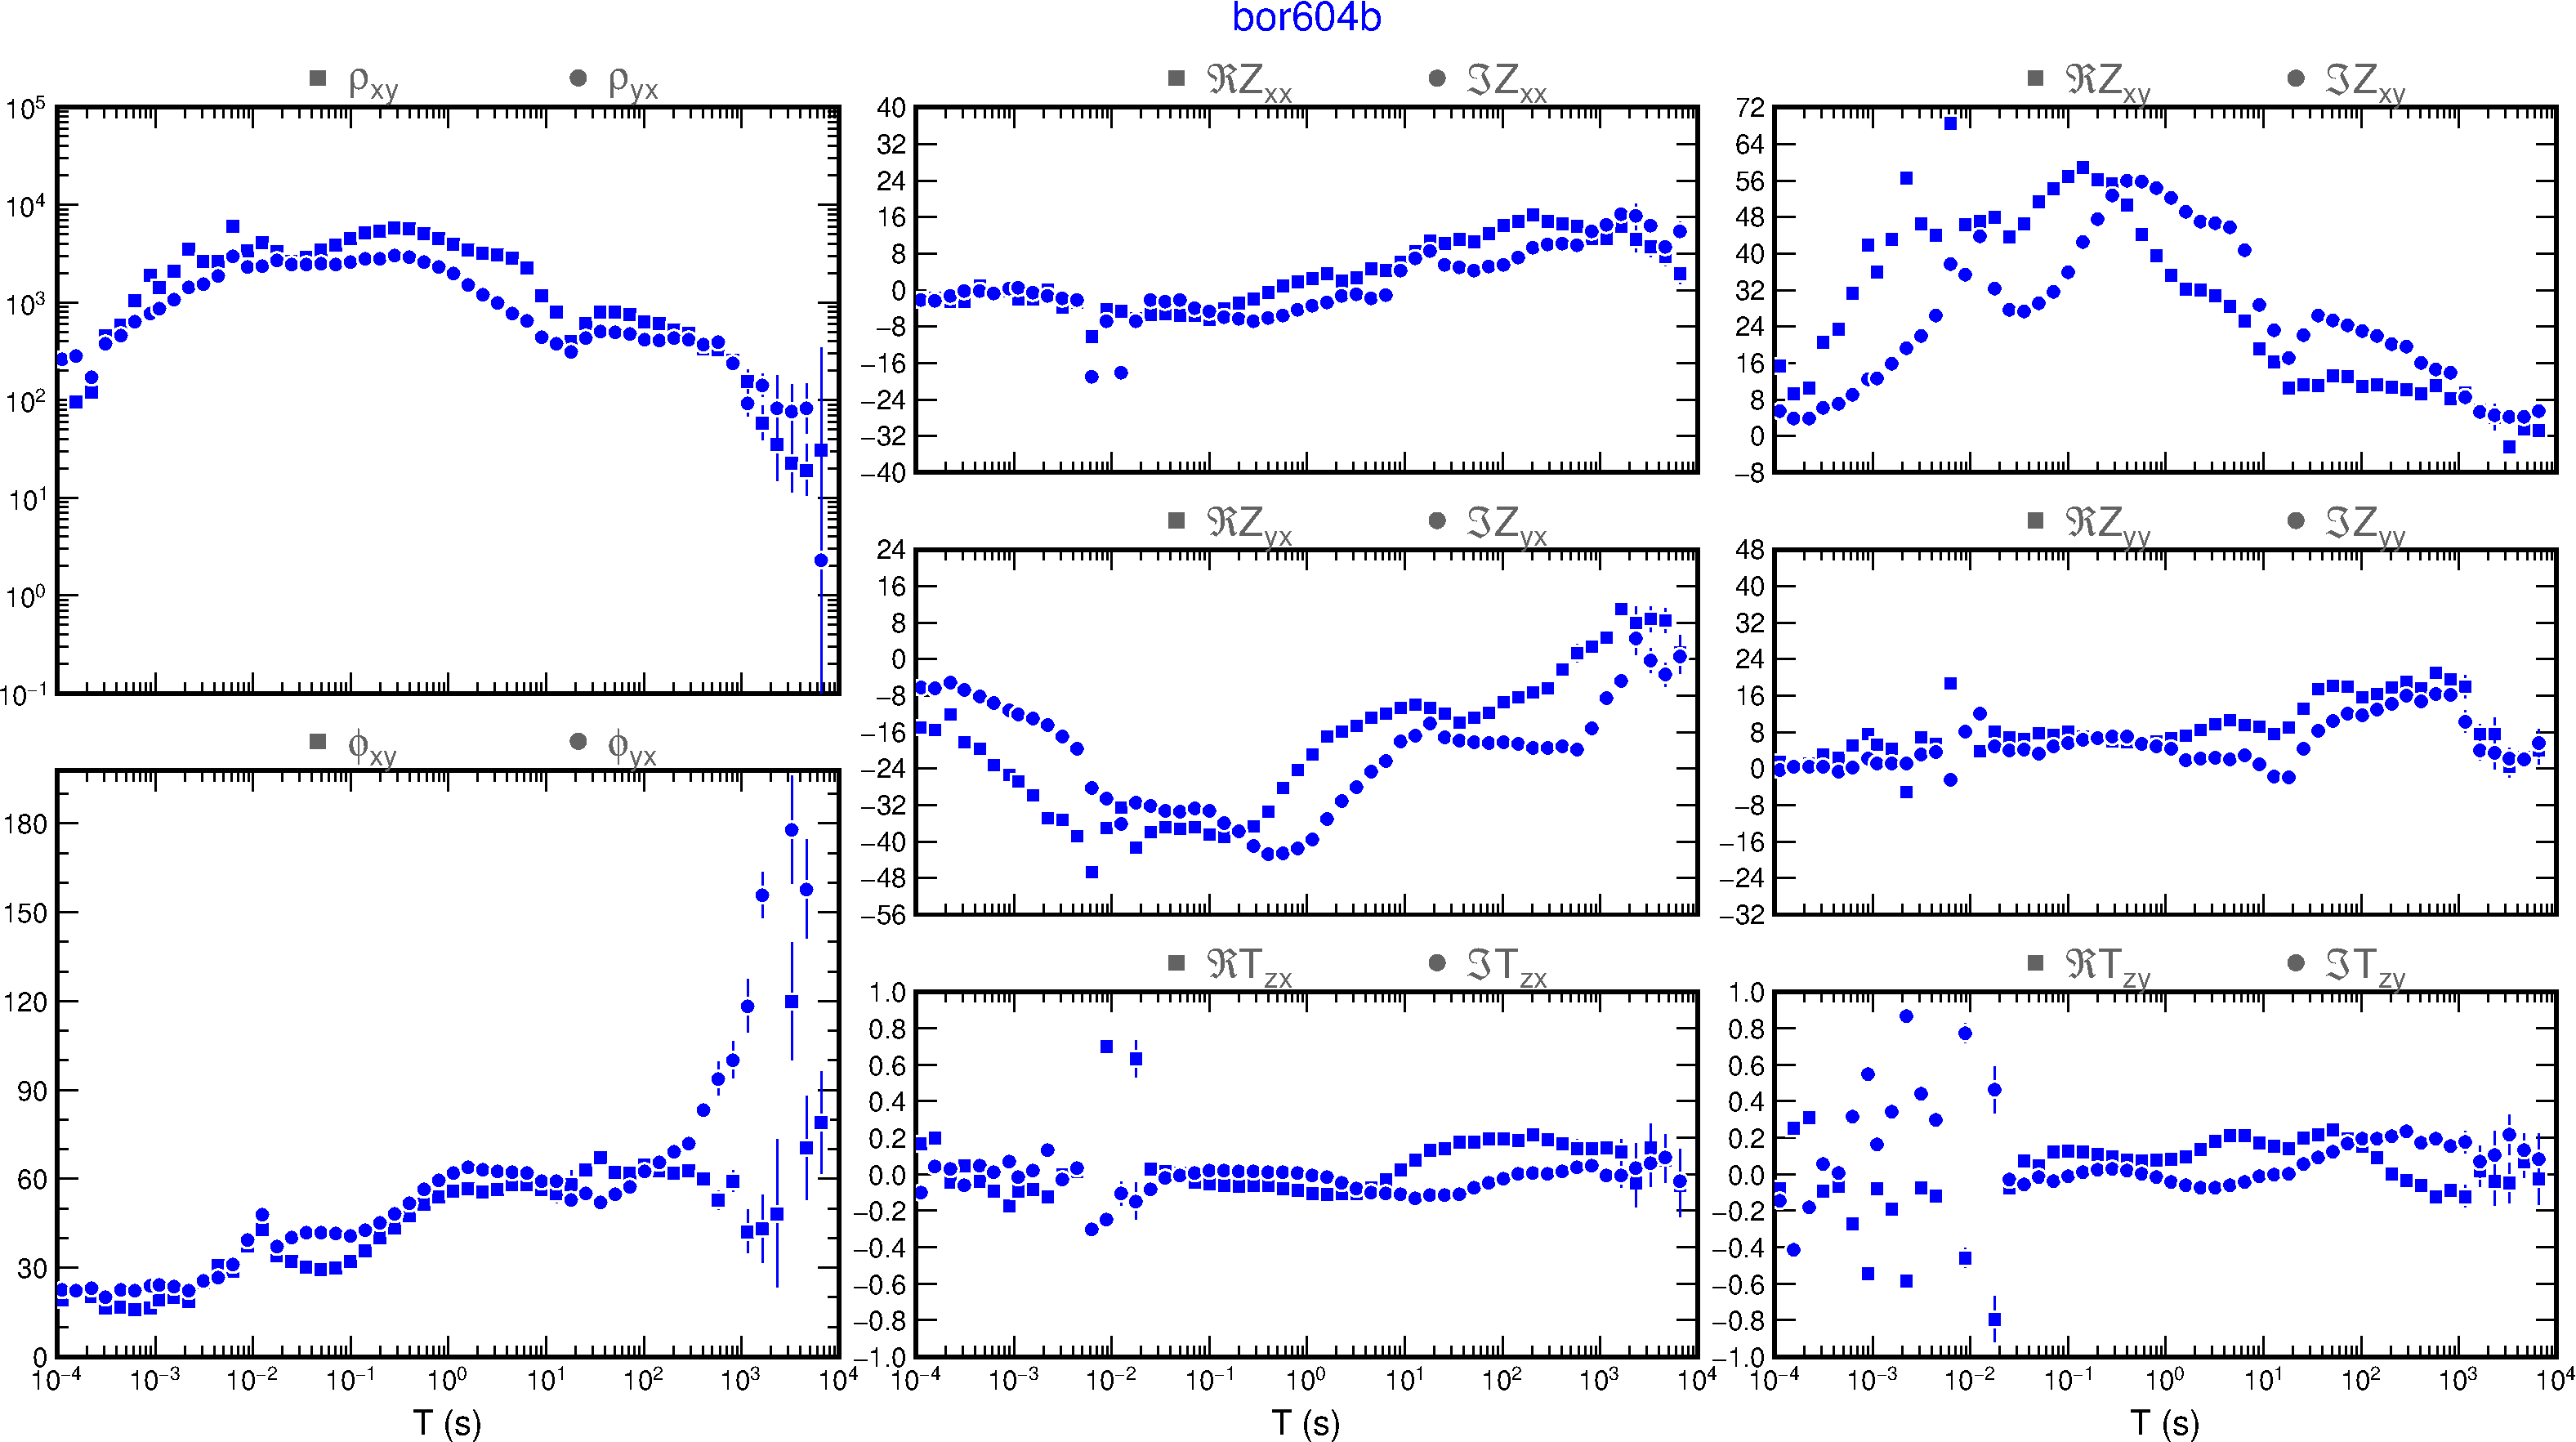
\includegraphics[width=16cm]{texto/figura/sites/M-bor604b.png}
            \end{center}
        \legend{\Fonte{\oautor.}}
    \end{figure}
    
    \begin{figure}[H]
        \caption{Manual -- bor605a}
            \begin{center}
                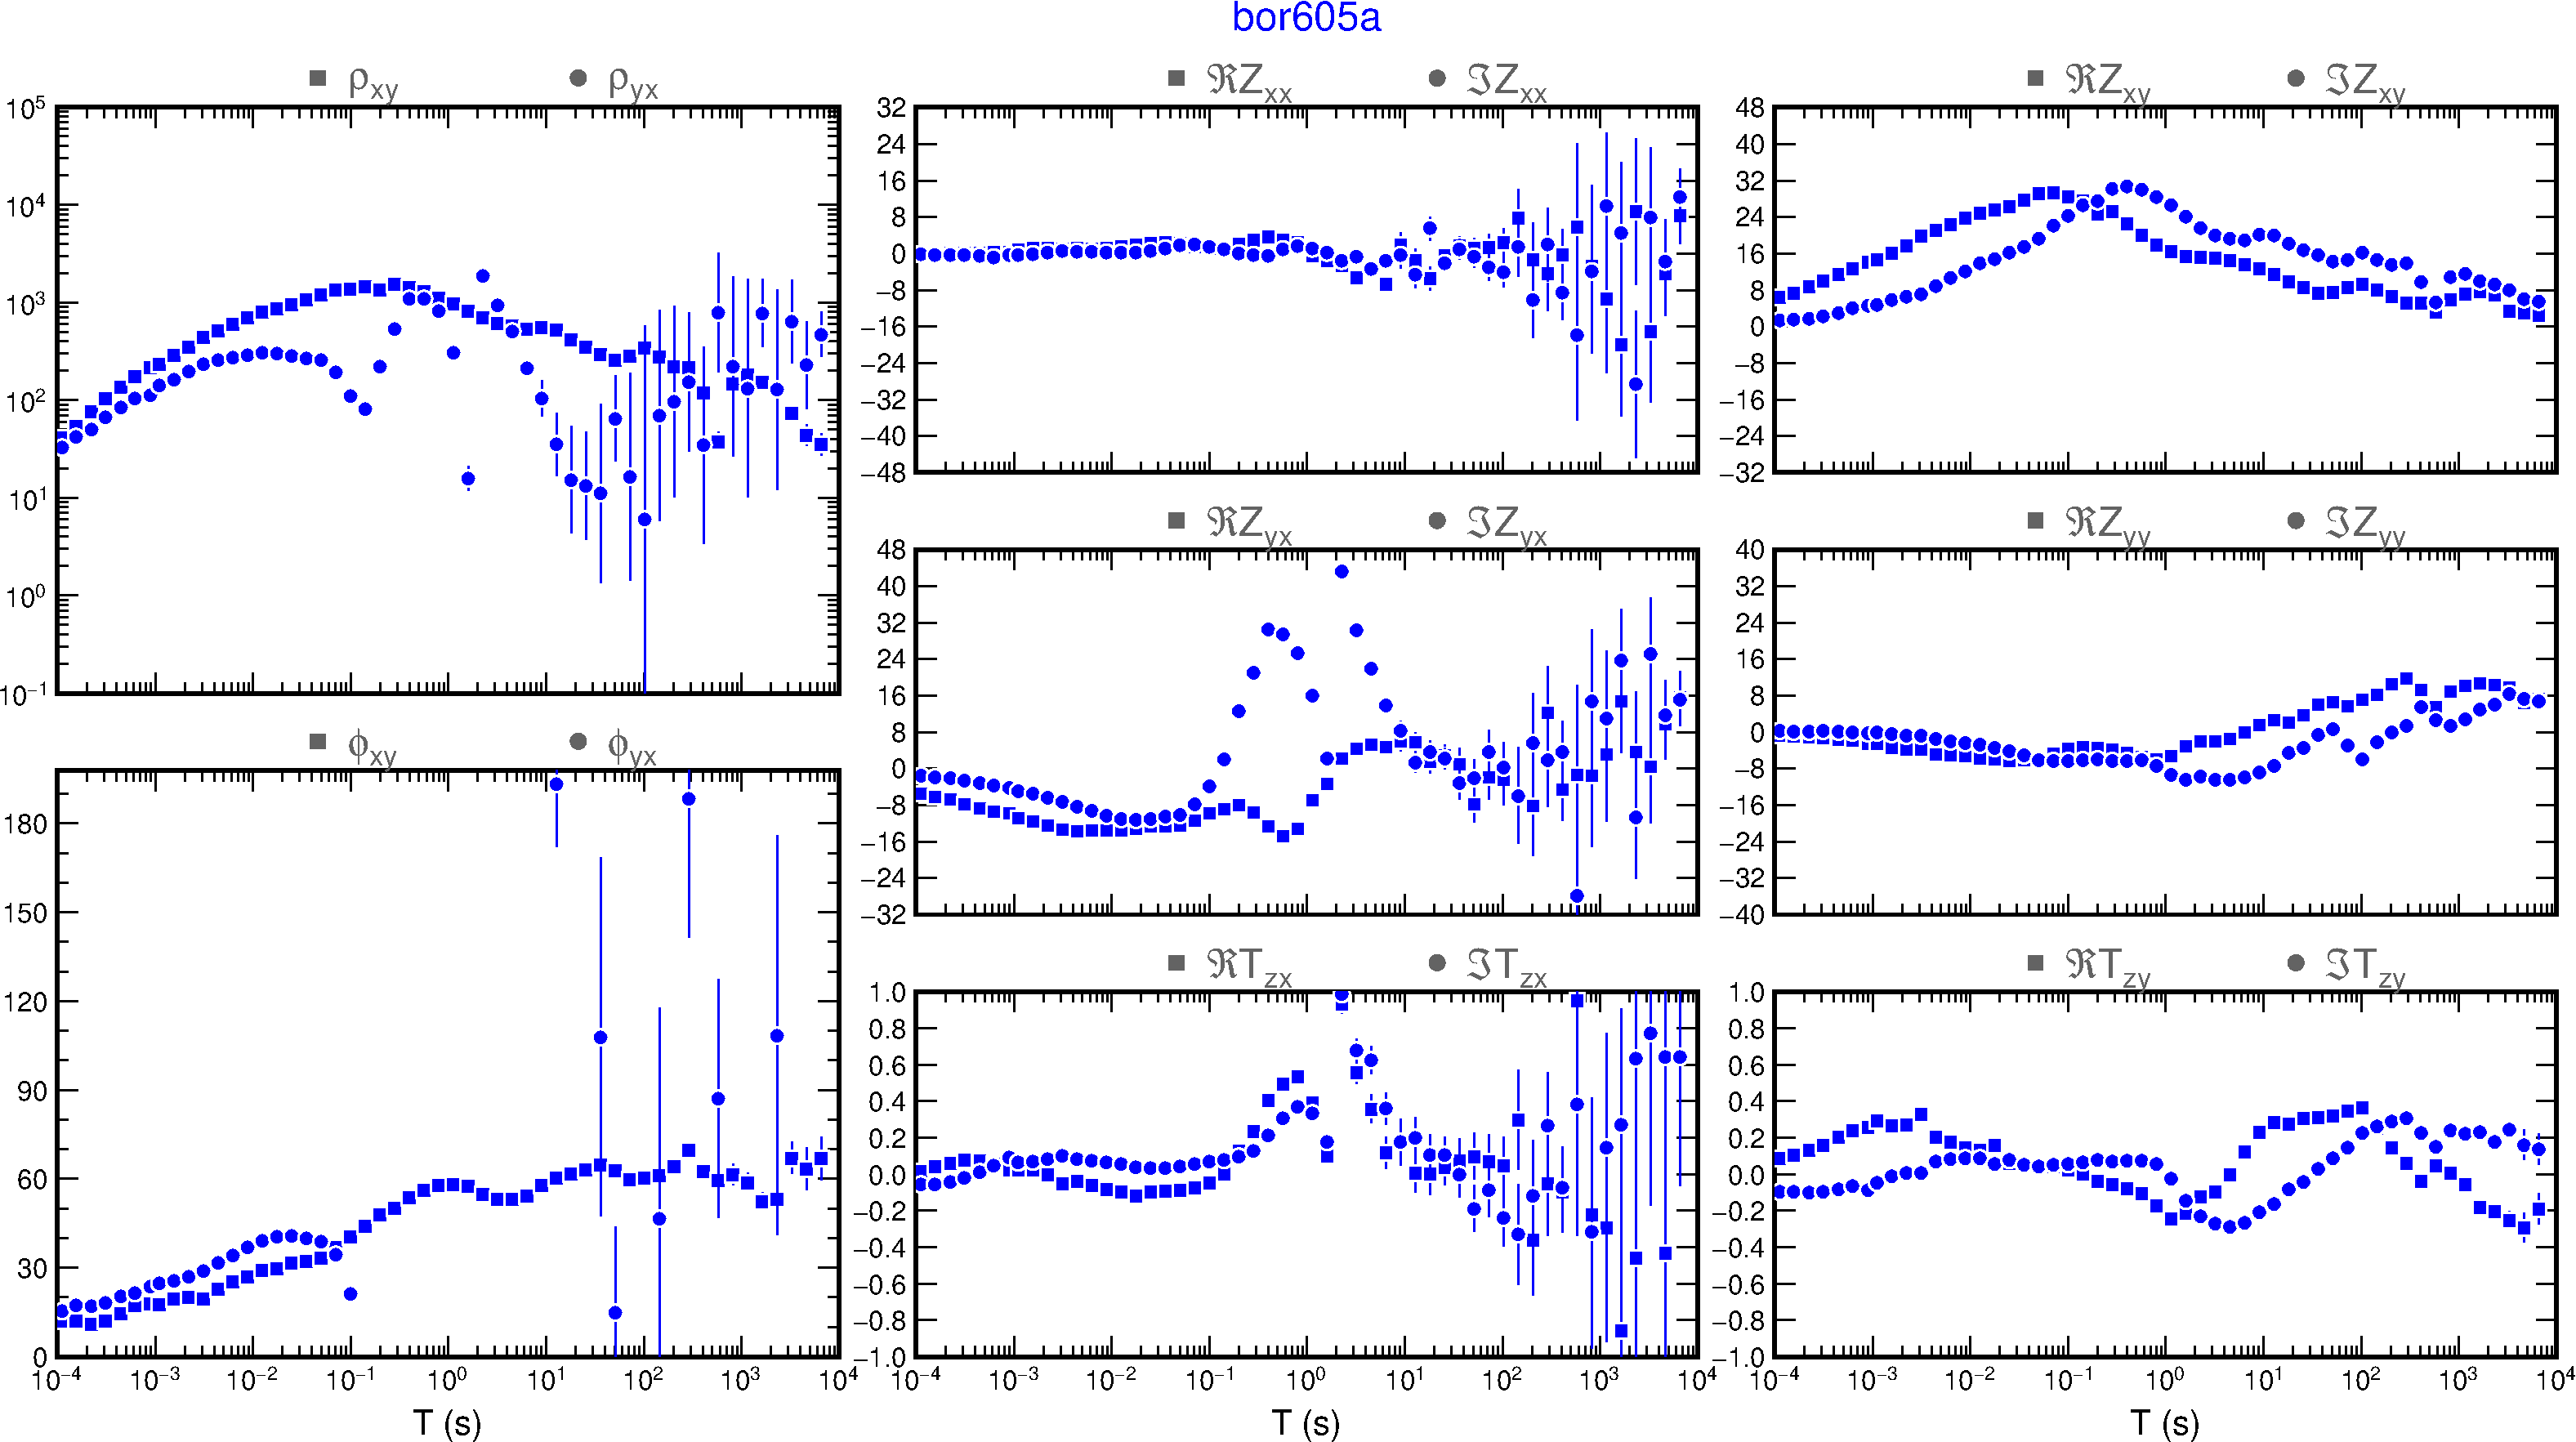
\includegraphics[width=16cm]{texto/figura/sites/M-bor605a.png}
            \end{center}
        \legend{\Fonte{\oautor.}}
    \end{figure}
    
    \begin{figure}[H]
        \caption{Manual -- bor605b}
            \begin{center}
                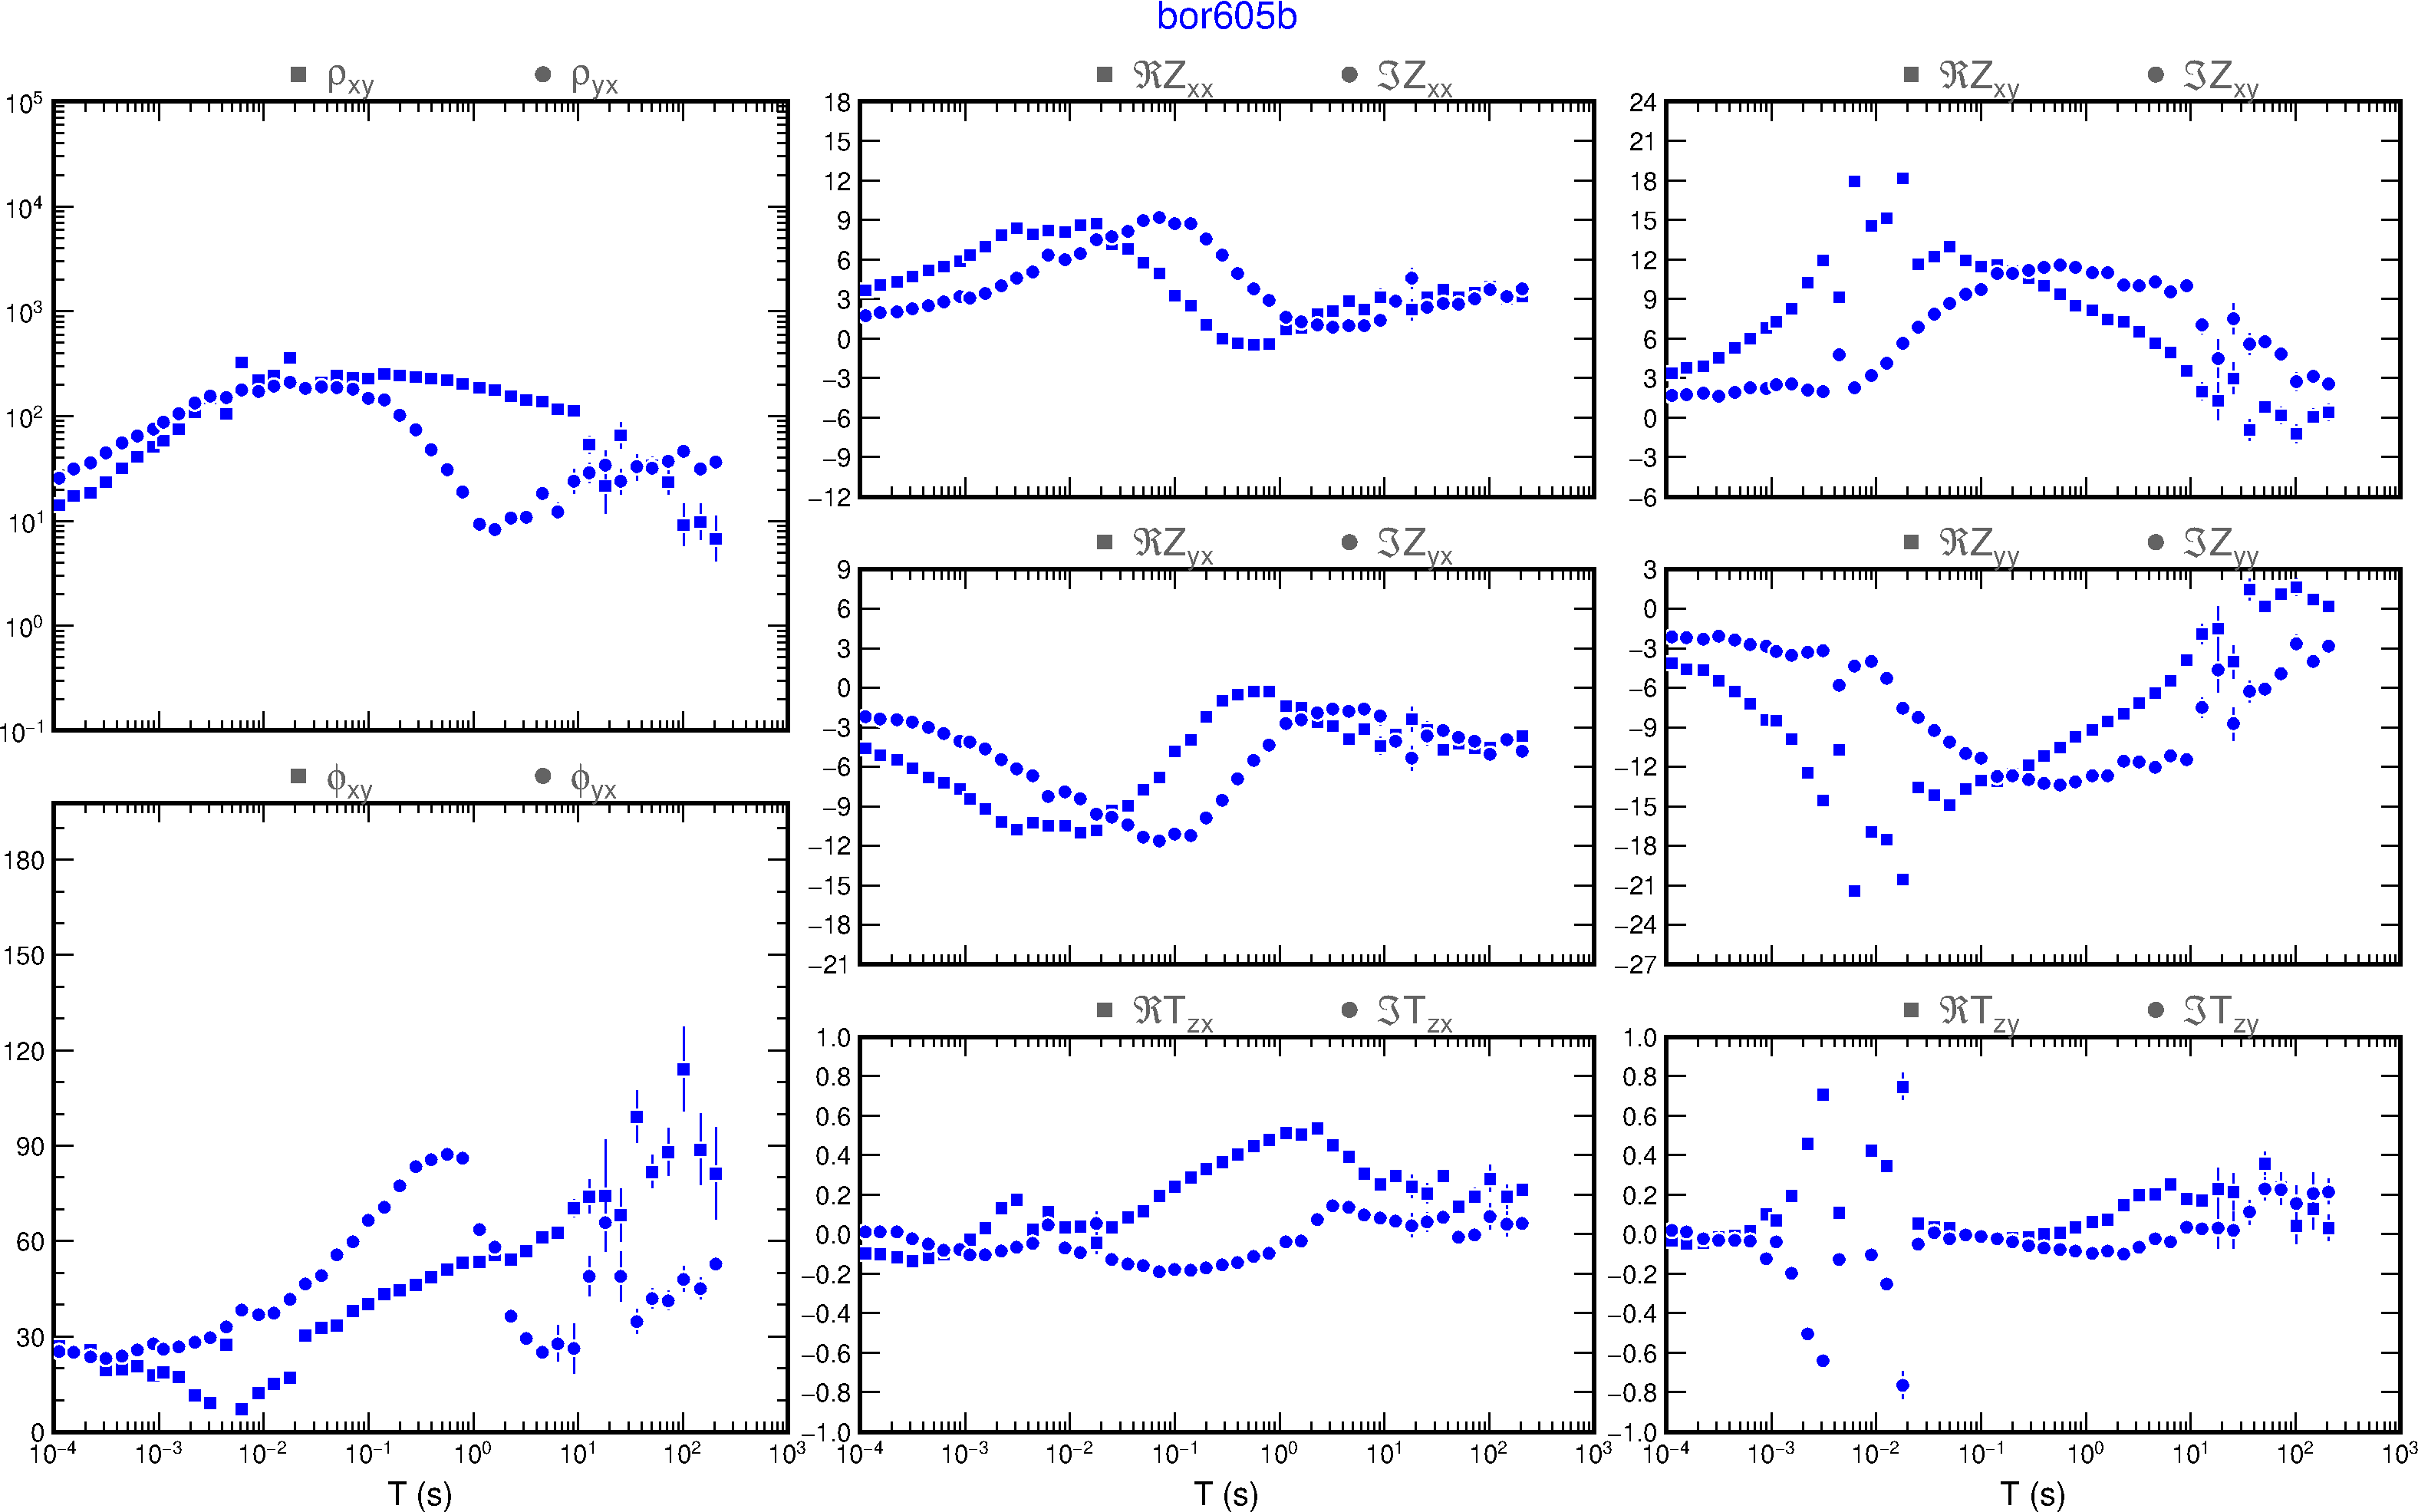
\includegraphics[width=15cm]{texto/figura/sites/M-bor605b.png}
            \end{center}
        \legend{\Fonte{\oautor.}}
    \end{figure}
    
    \begin{figure}[H]
        \caption{Manual -- bor606a}
            \begin{center}
                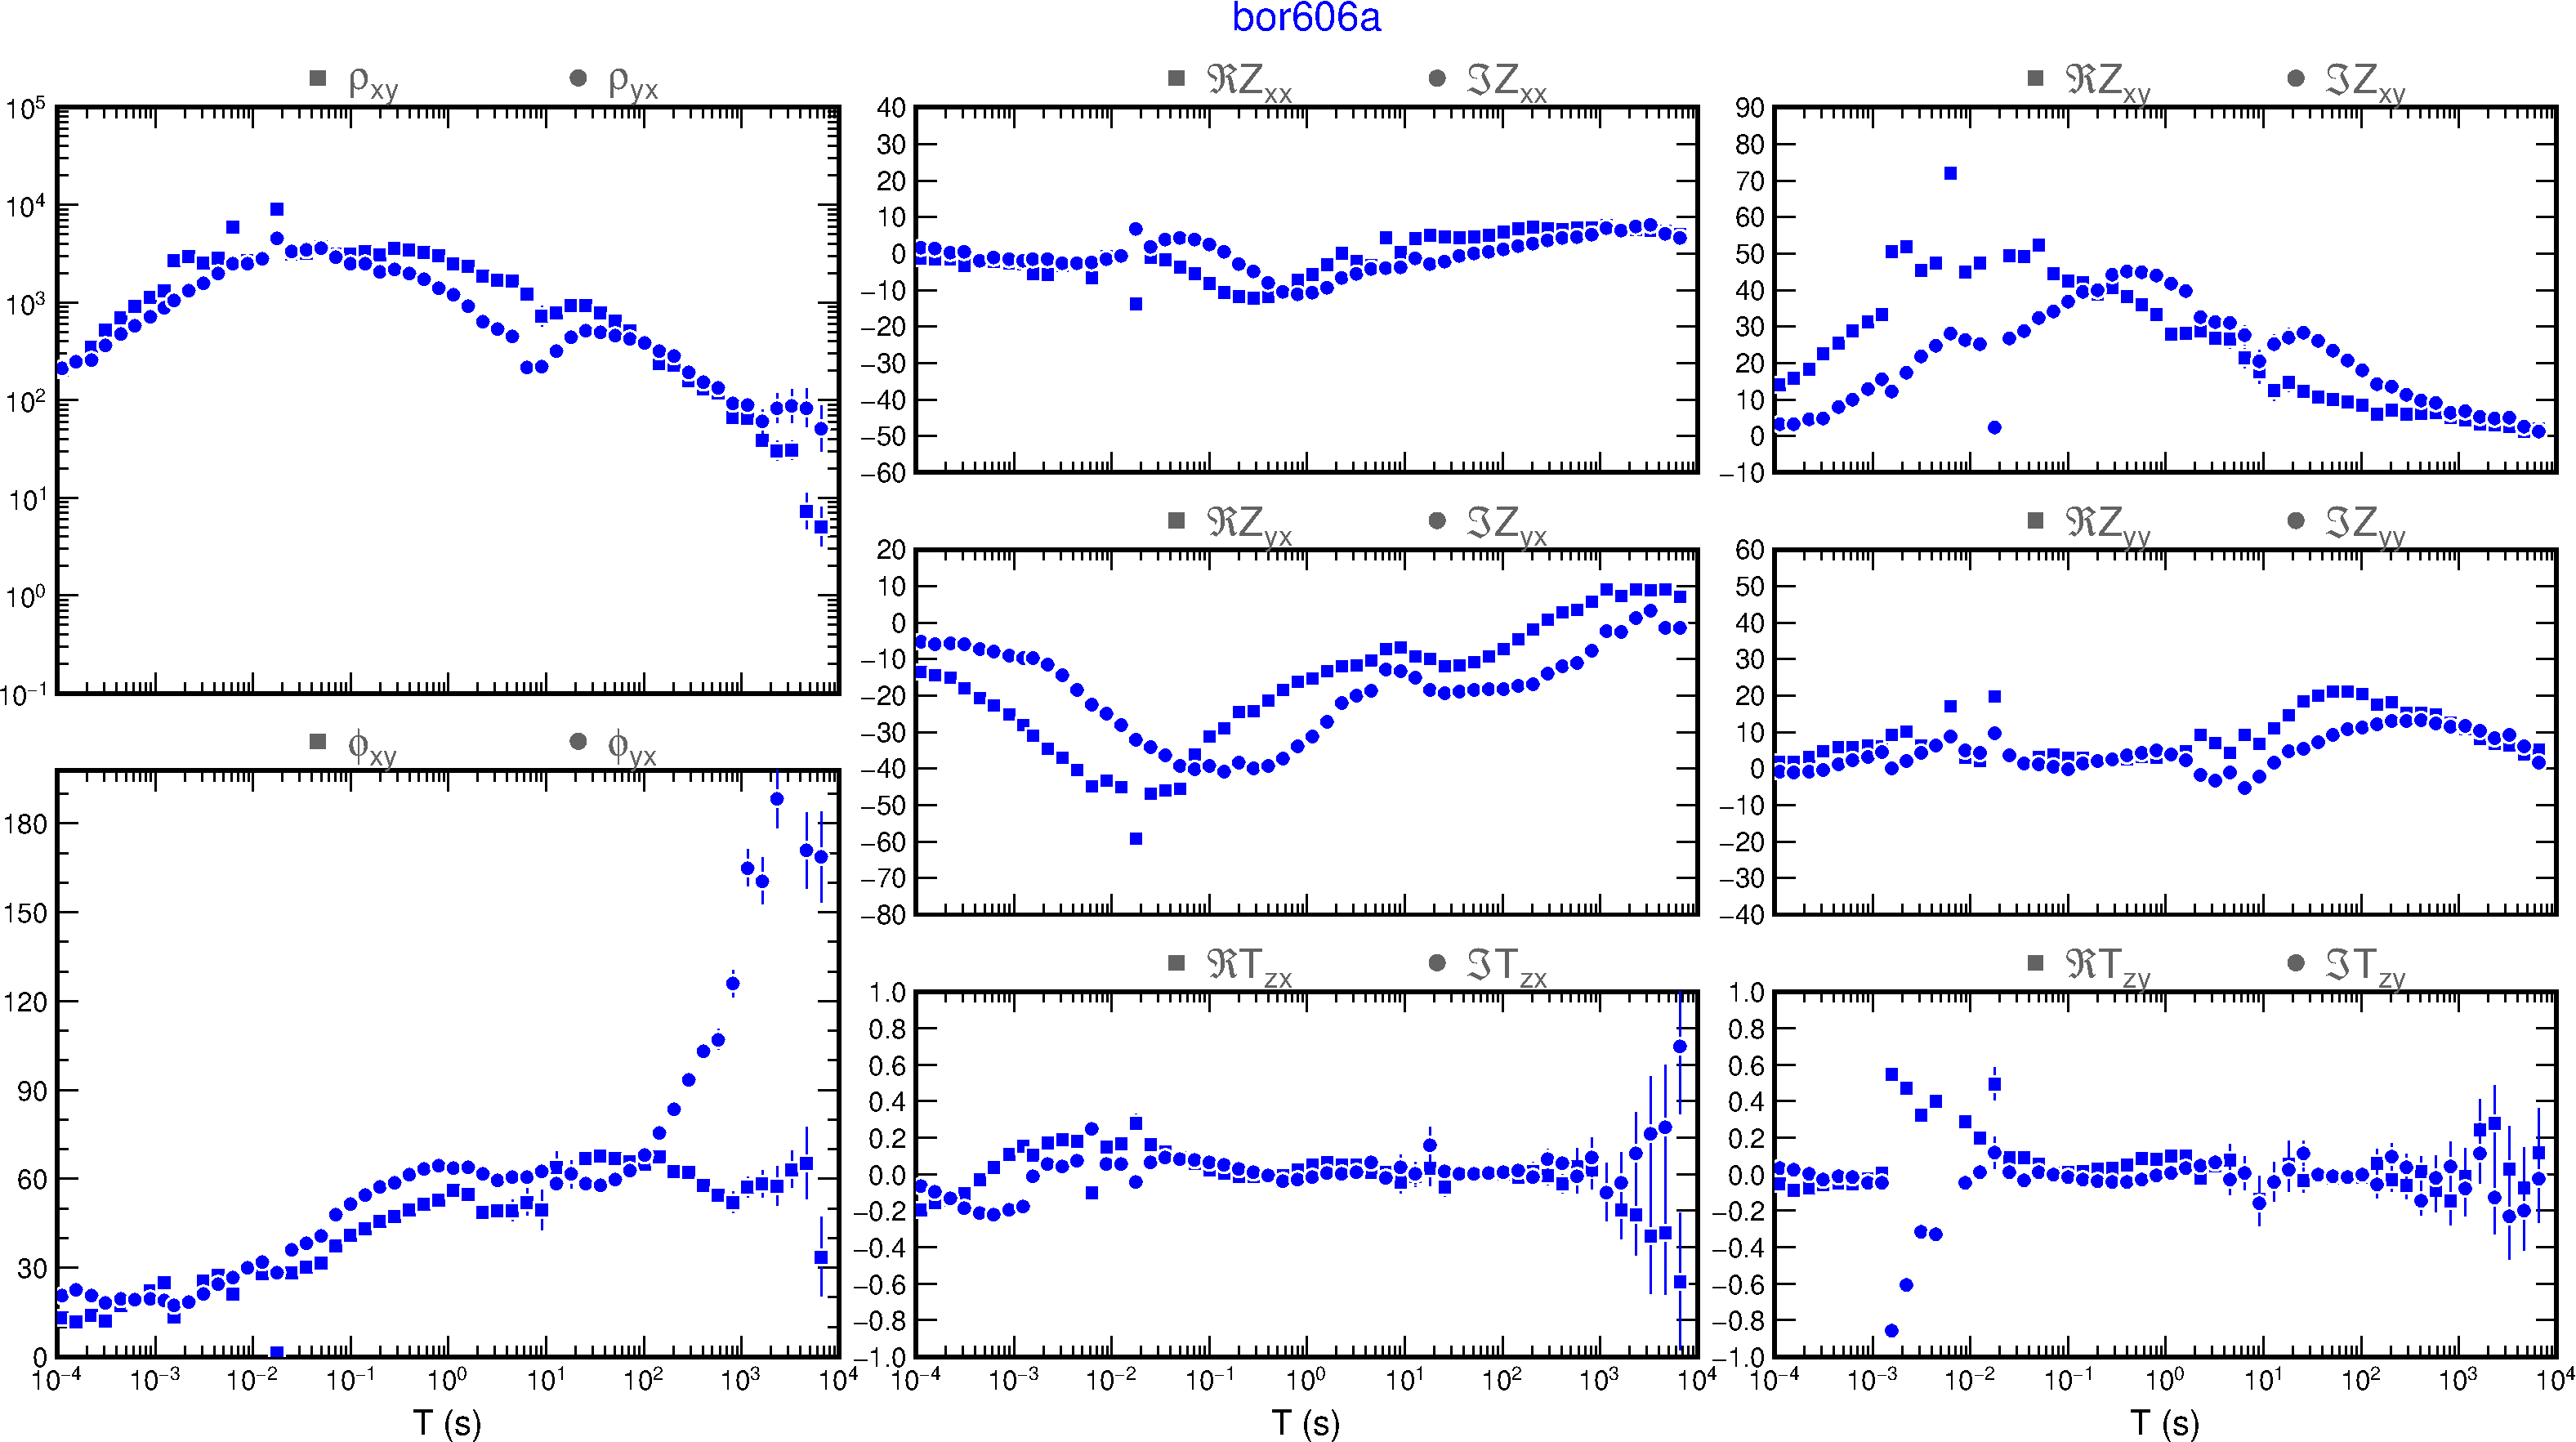
\includegraphics[width=15cm]{texto/figura/sites/M-bor606a.png}
            \end{center}
        \legend{\Fonte{\oautor.}}
    \end{figure}
    
    \begin{figure}[H]
        \caption{Manual -- bor606b}
            \begin{center}
                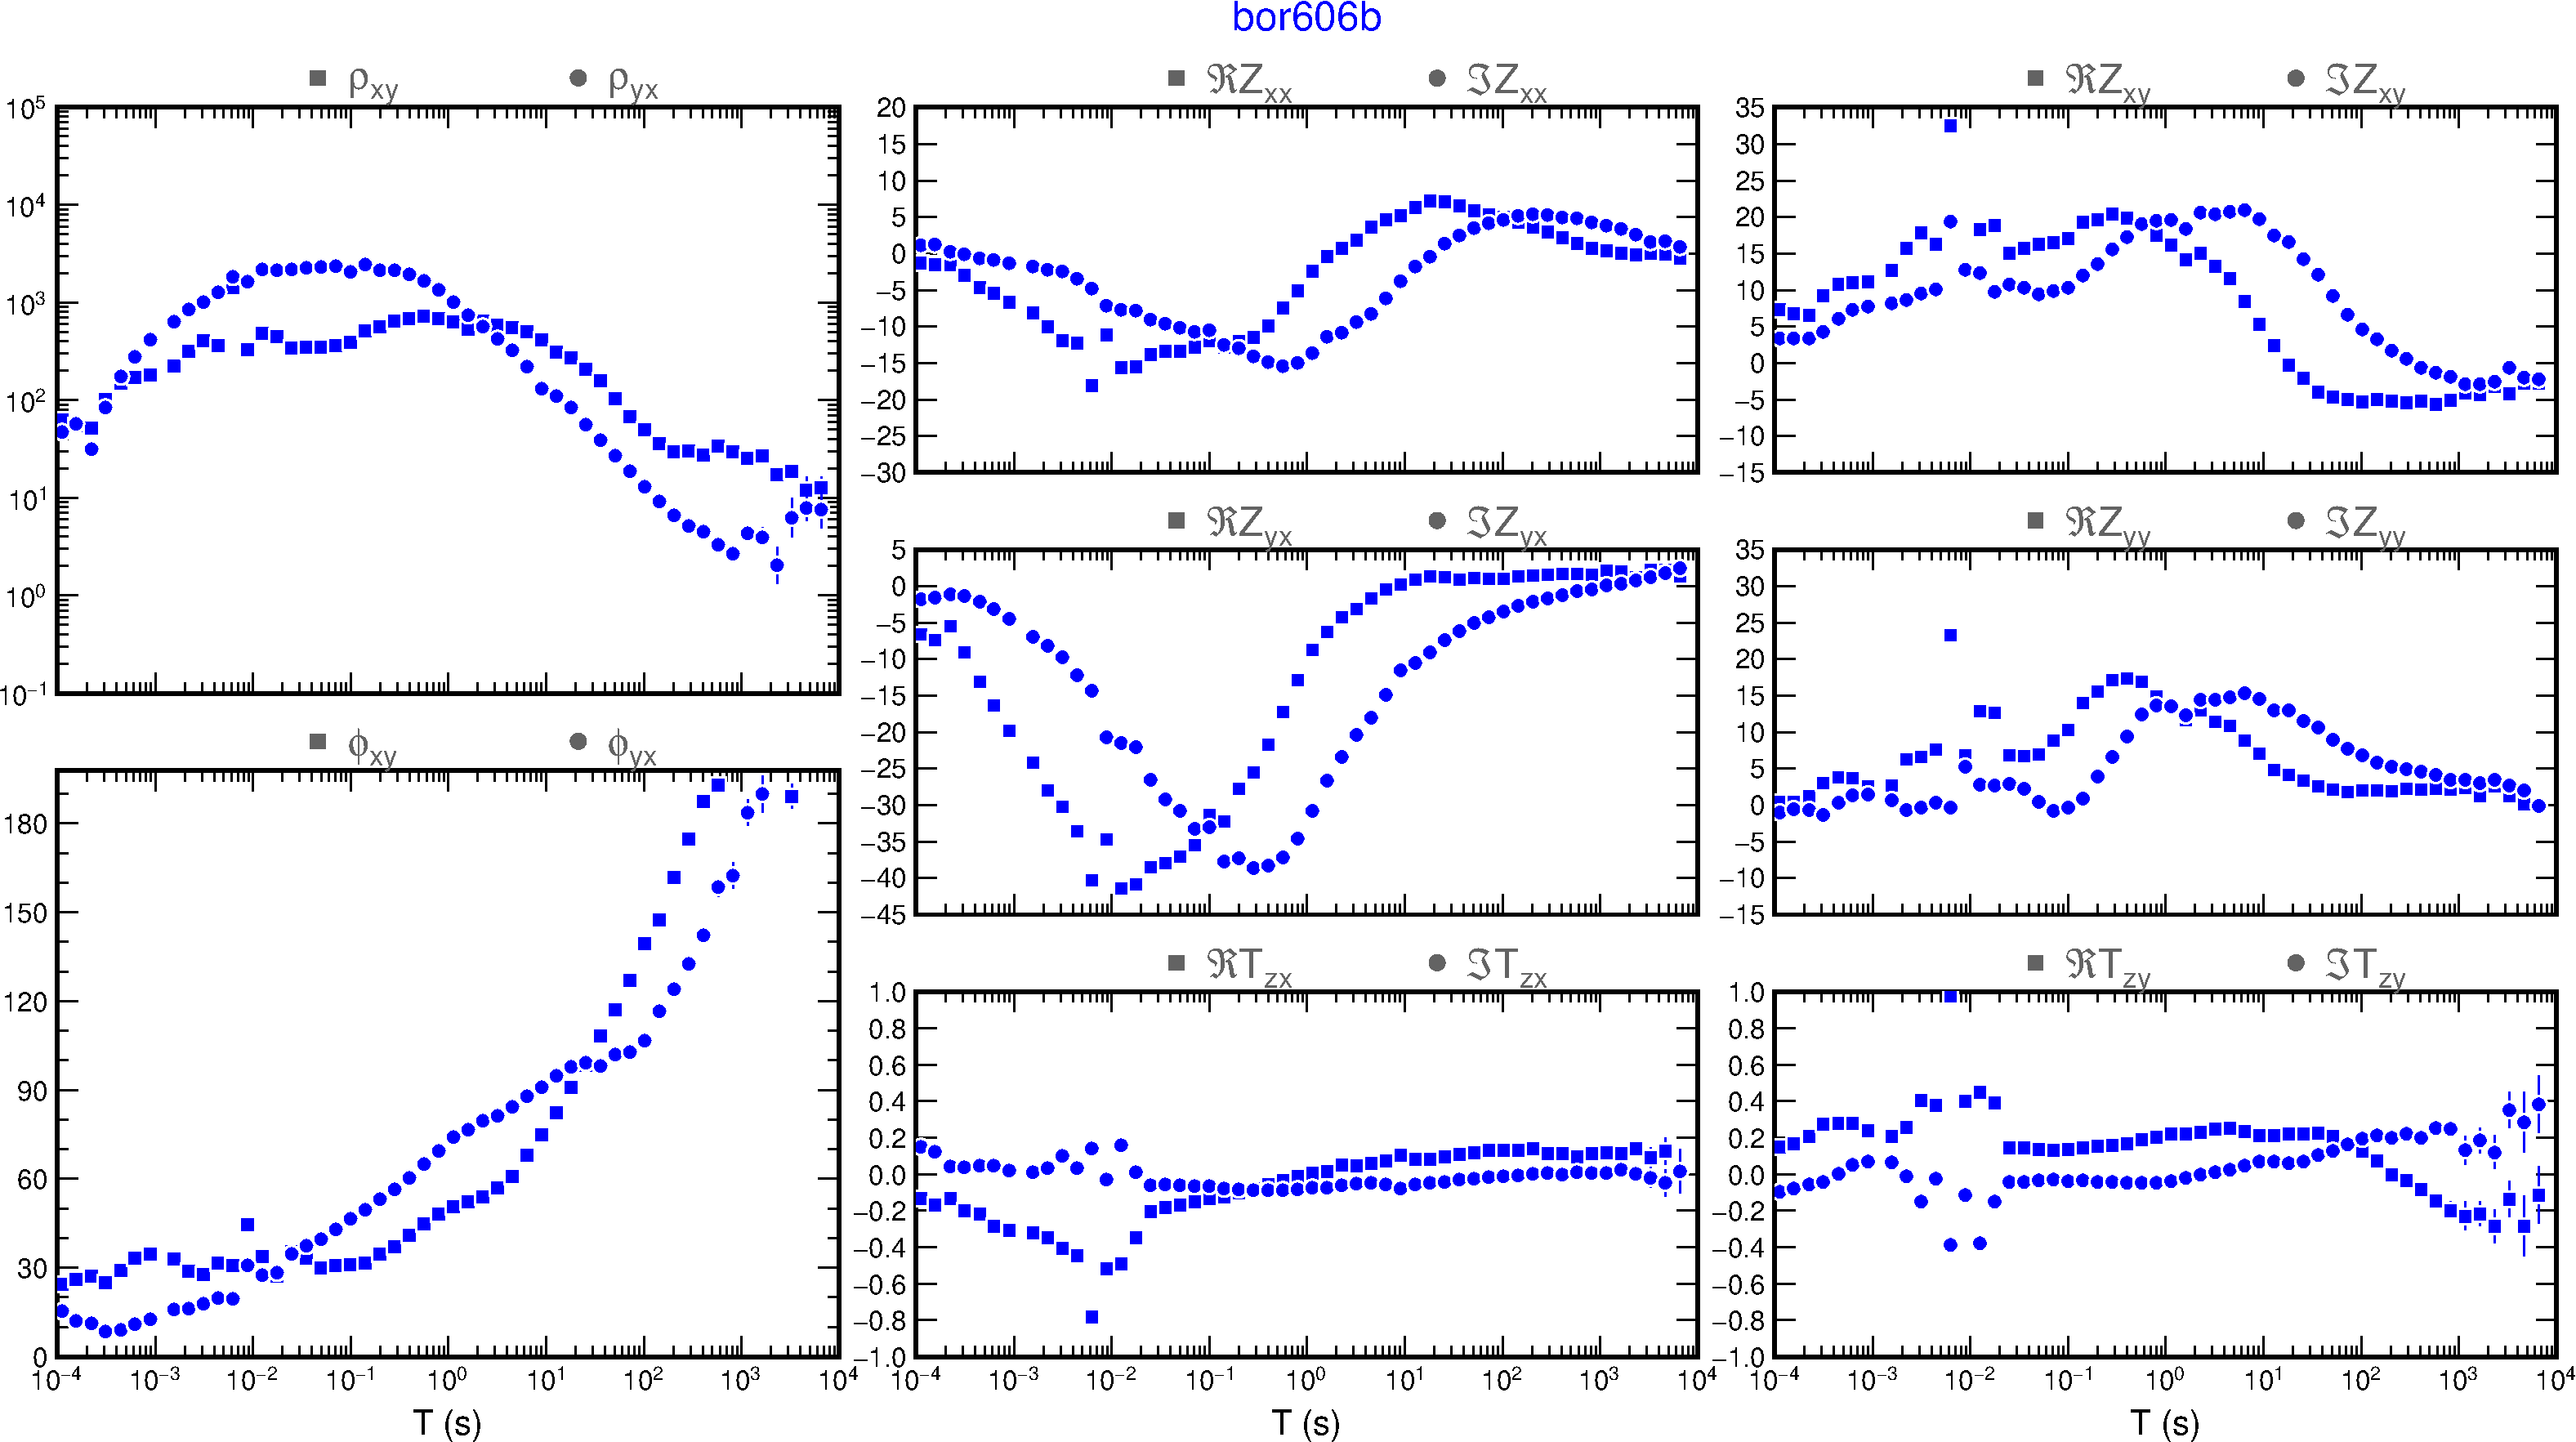
\includegraphics[width=16cm]{texto/figura/sites/M-bor606b.png}
            \end{center}
        \legend{\Fonte{\oautor.}}
    \end{figure}
    
    \begin{figure}[H]
        \caption{Manual -- bor607a}
            \begin{center}
                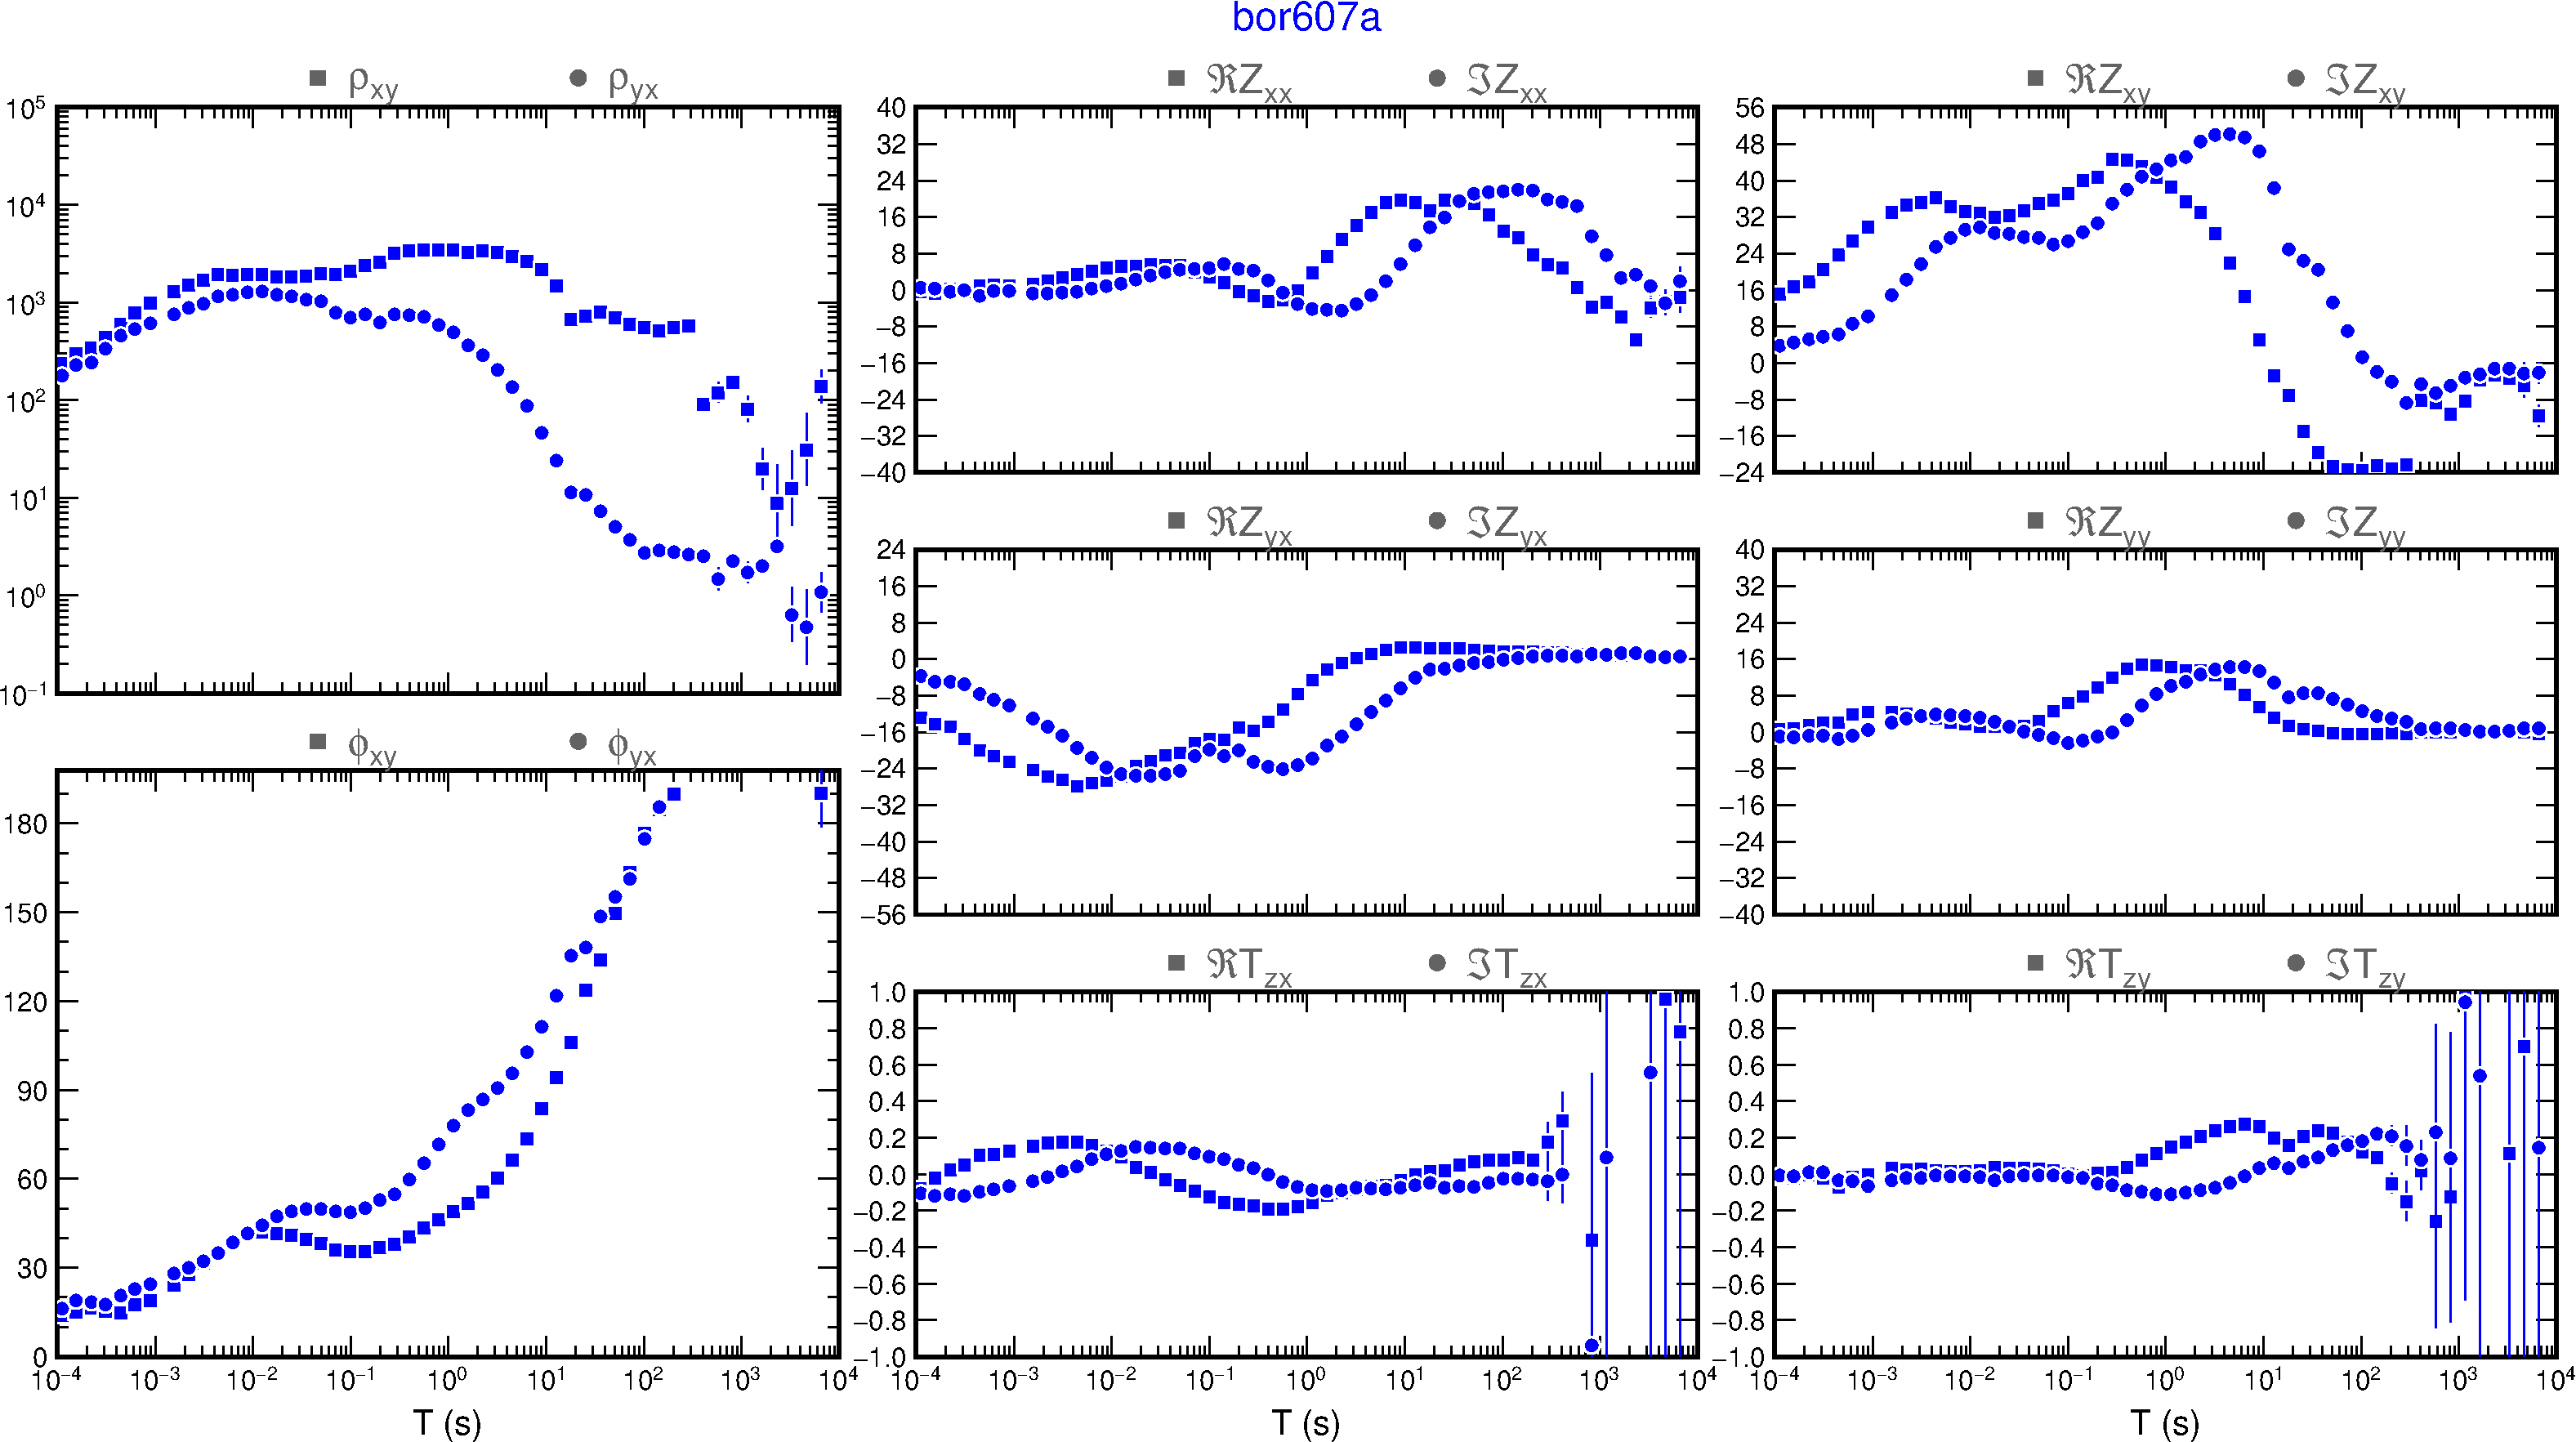
\includegraphics[width=16cm]{texto/figura/sites/M-bor607a.png}
            \end{center}
        \legend{\Fonte{\oautor.}}
    \end{figure}
    
    \begin{figure}[H]
        \caption{Manual -- bor607b}
            \begin{center}
                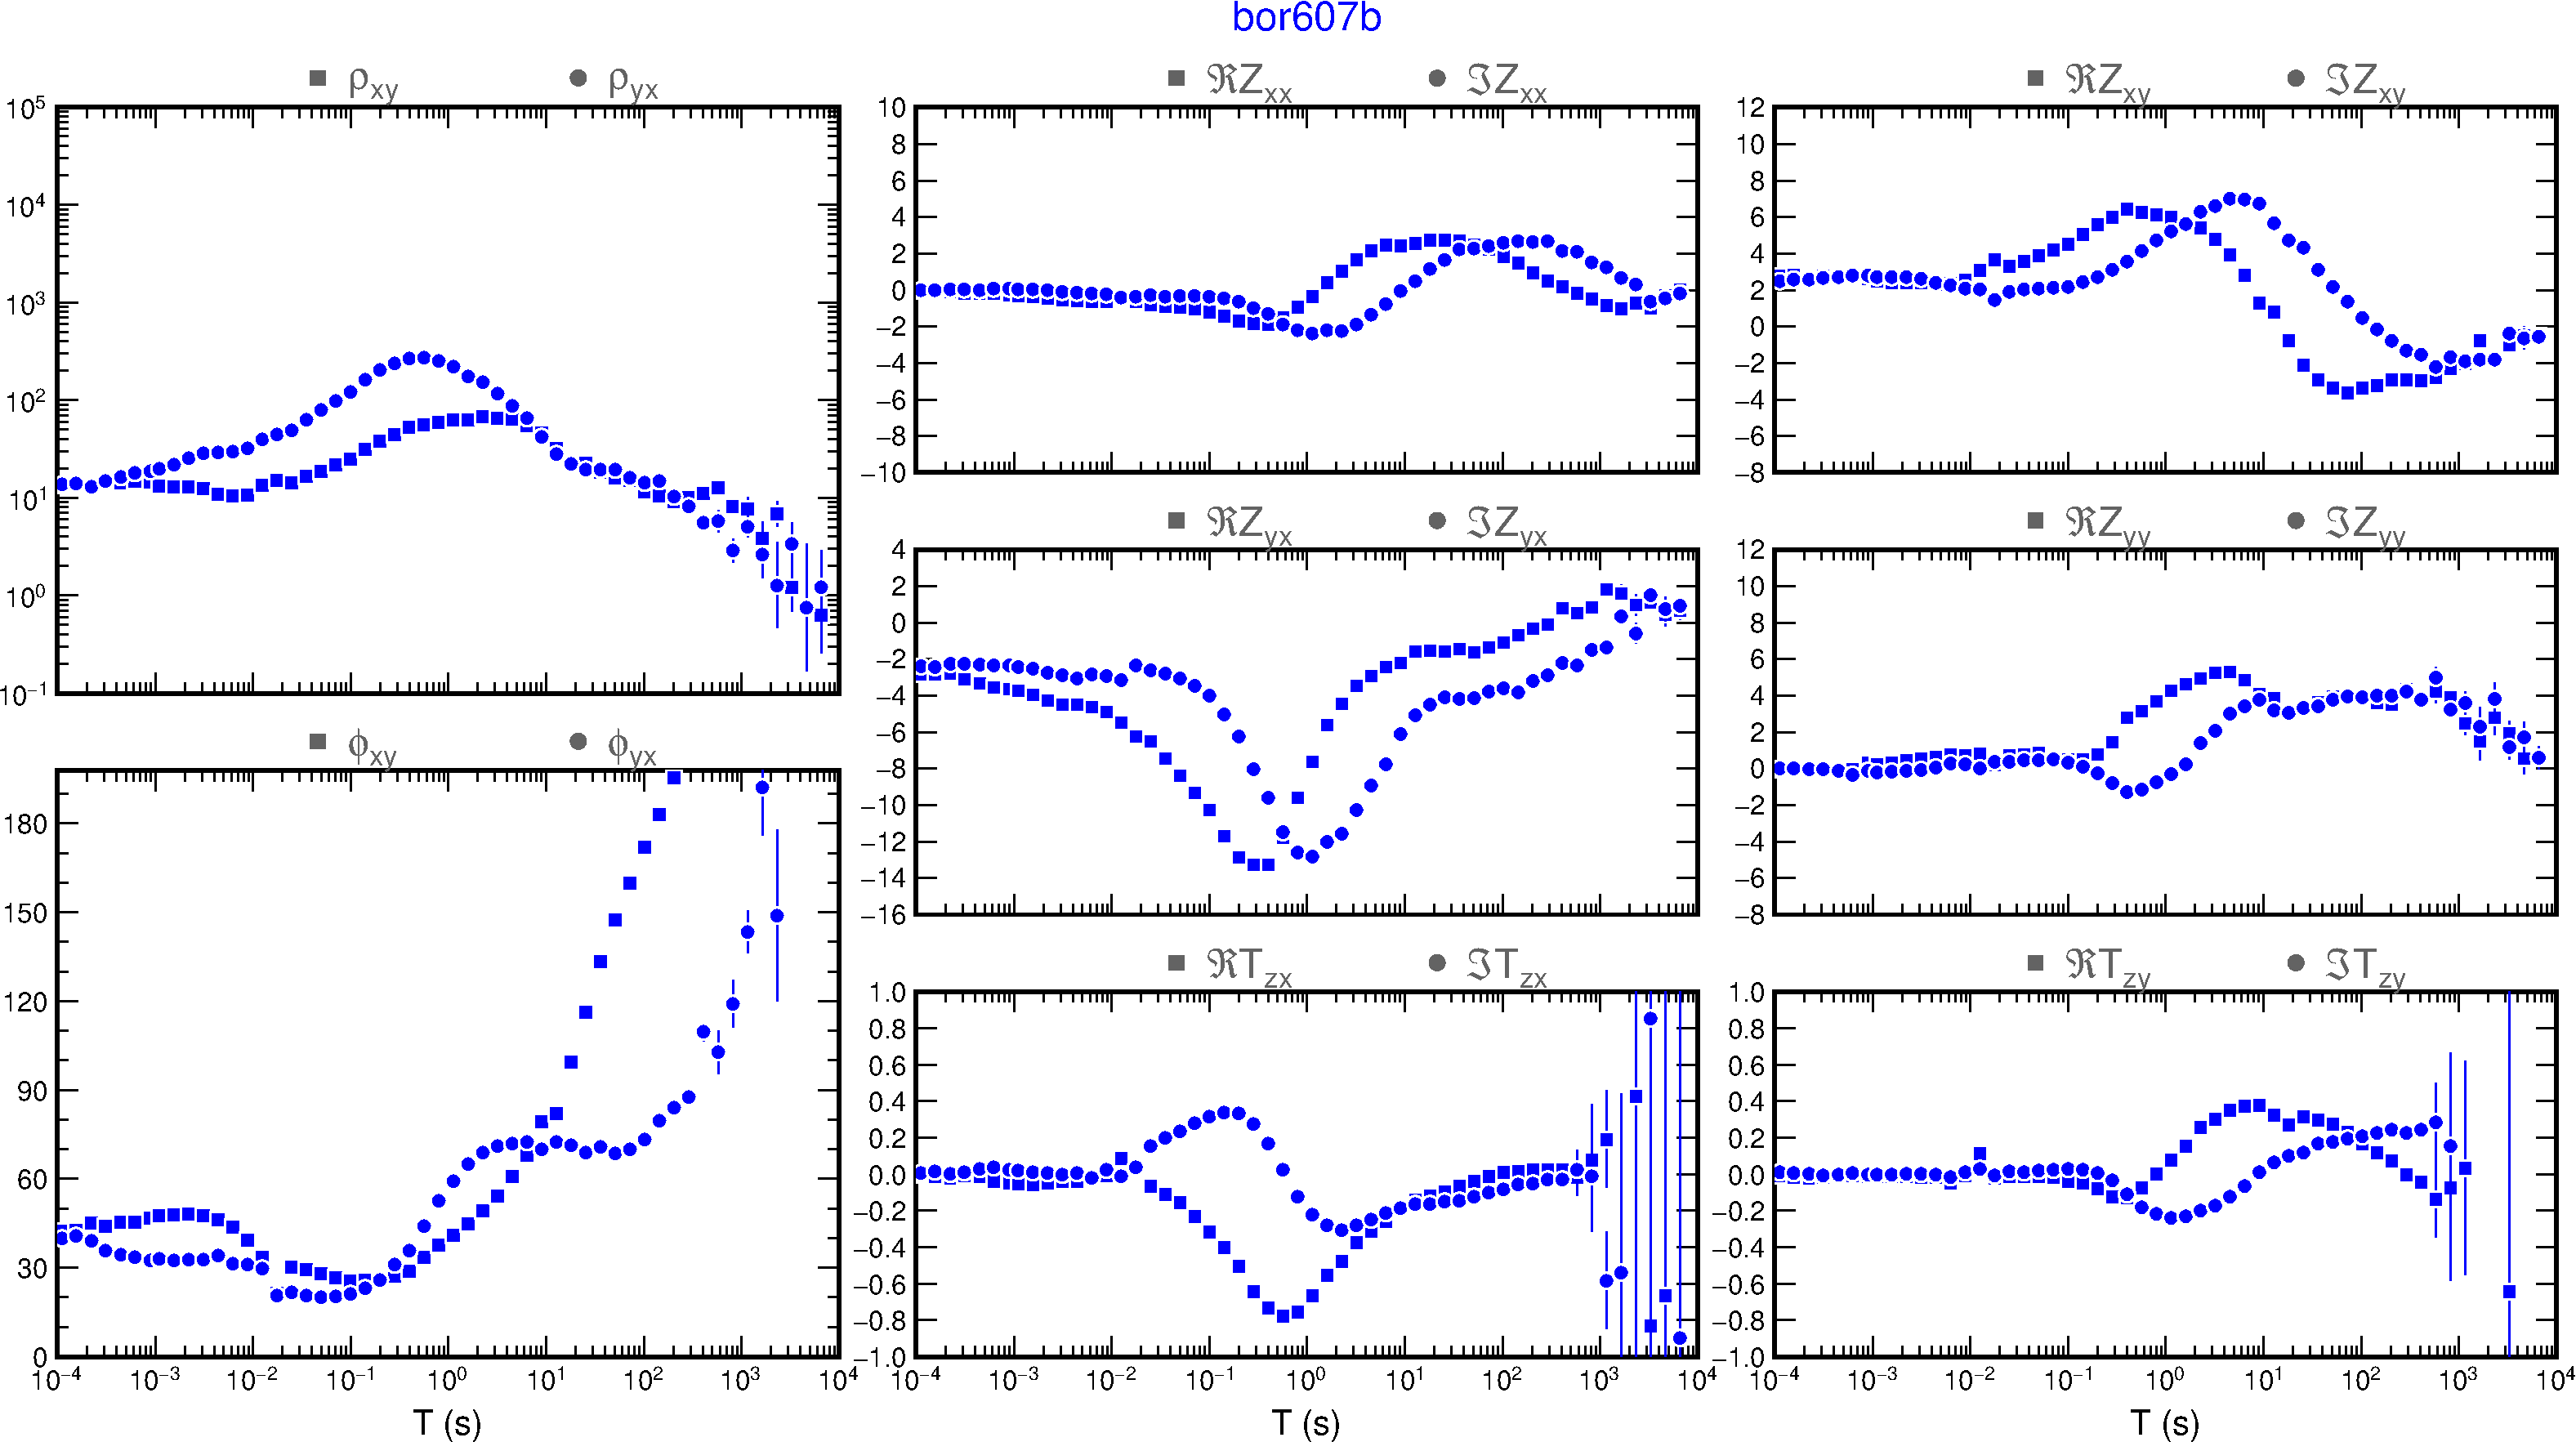
\includegraphics[width=16cm]{texto/figura/sites/M-bor607b.png}
            \end{center}
        \legend{\Fonte{\oautor.}}
    \end{figure}
    
    \begin{figure}[H]
        \caption{Manual -- bor608a}
            \begin{center}
                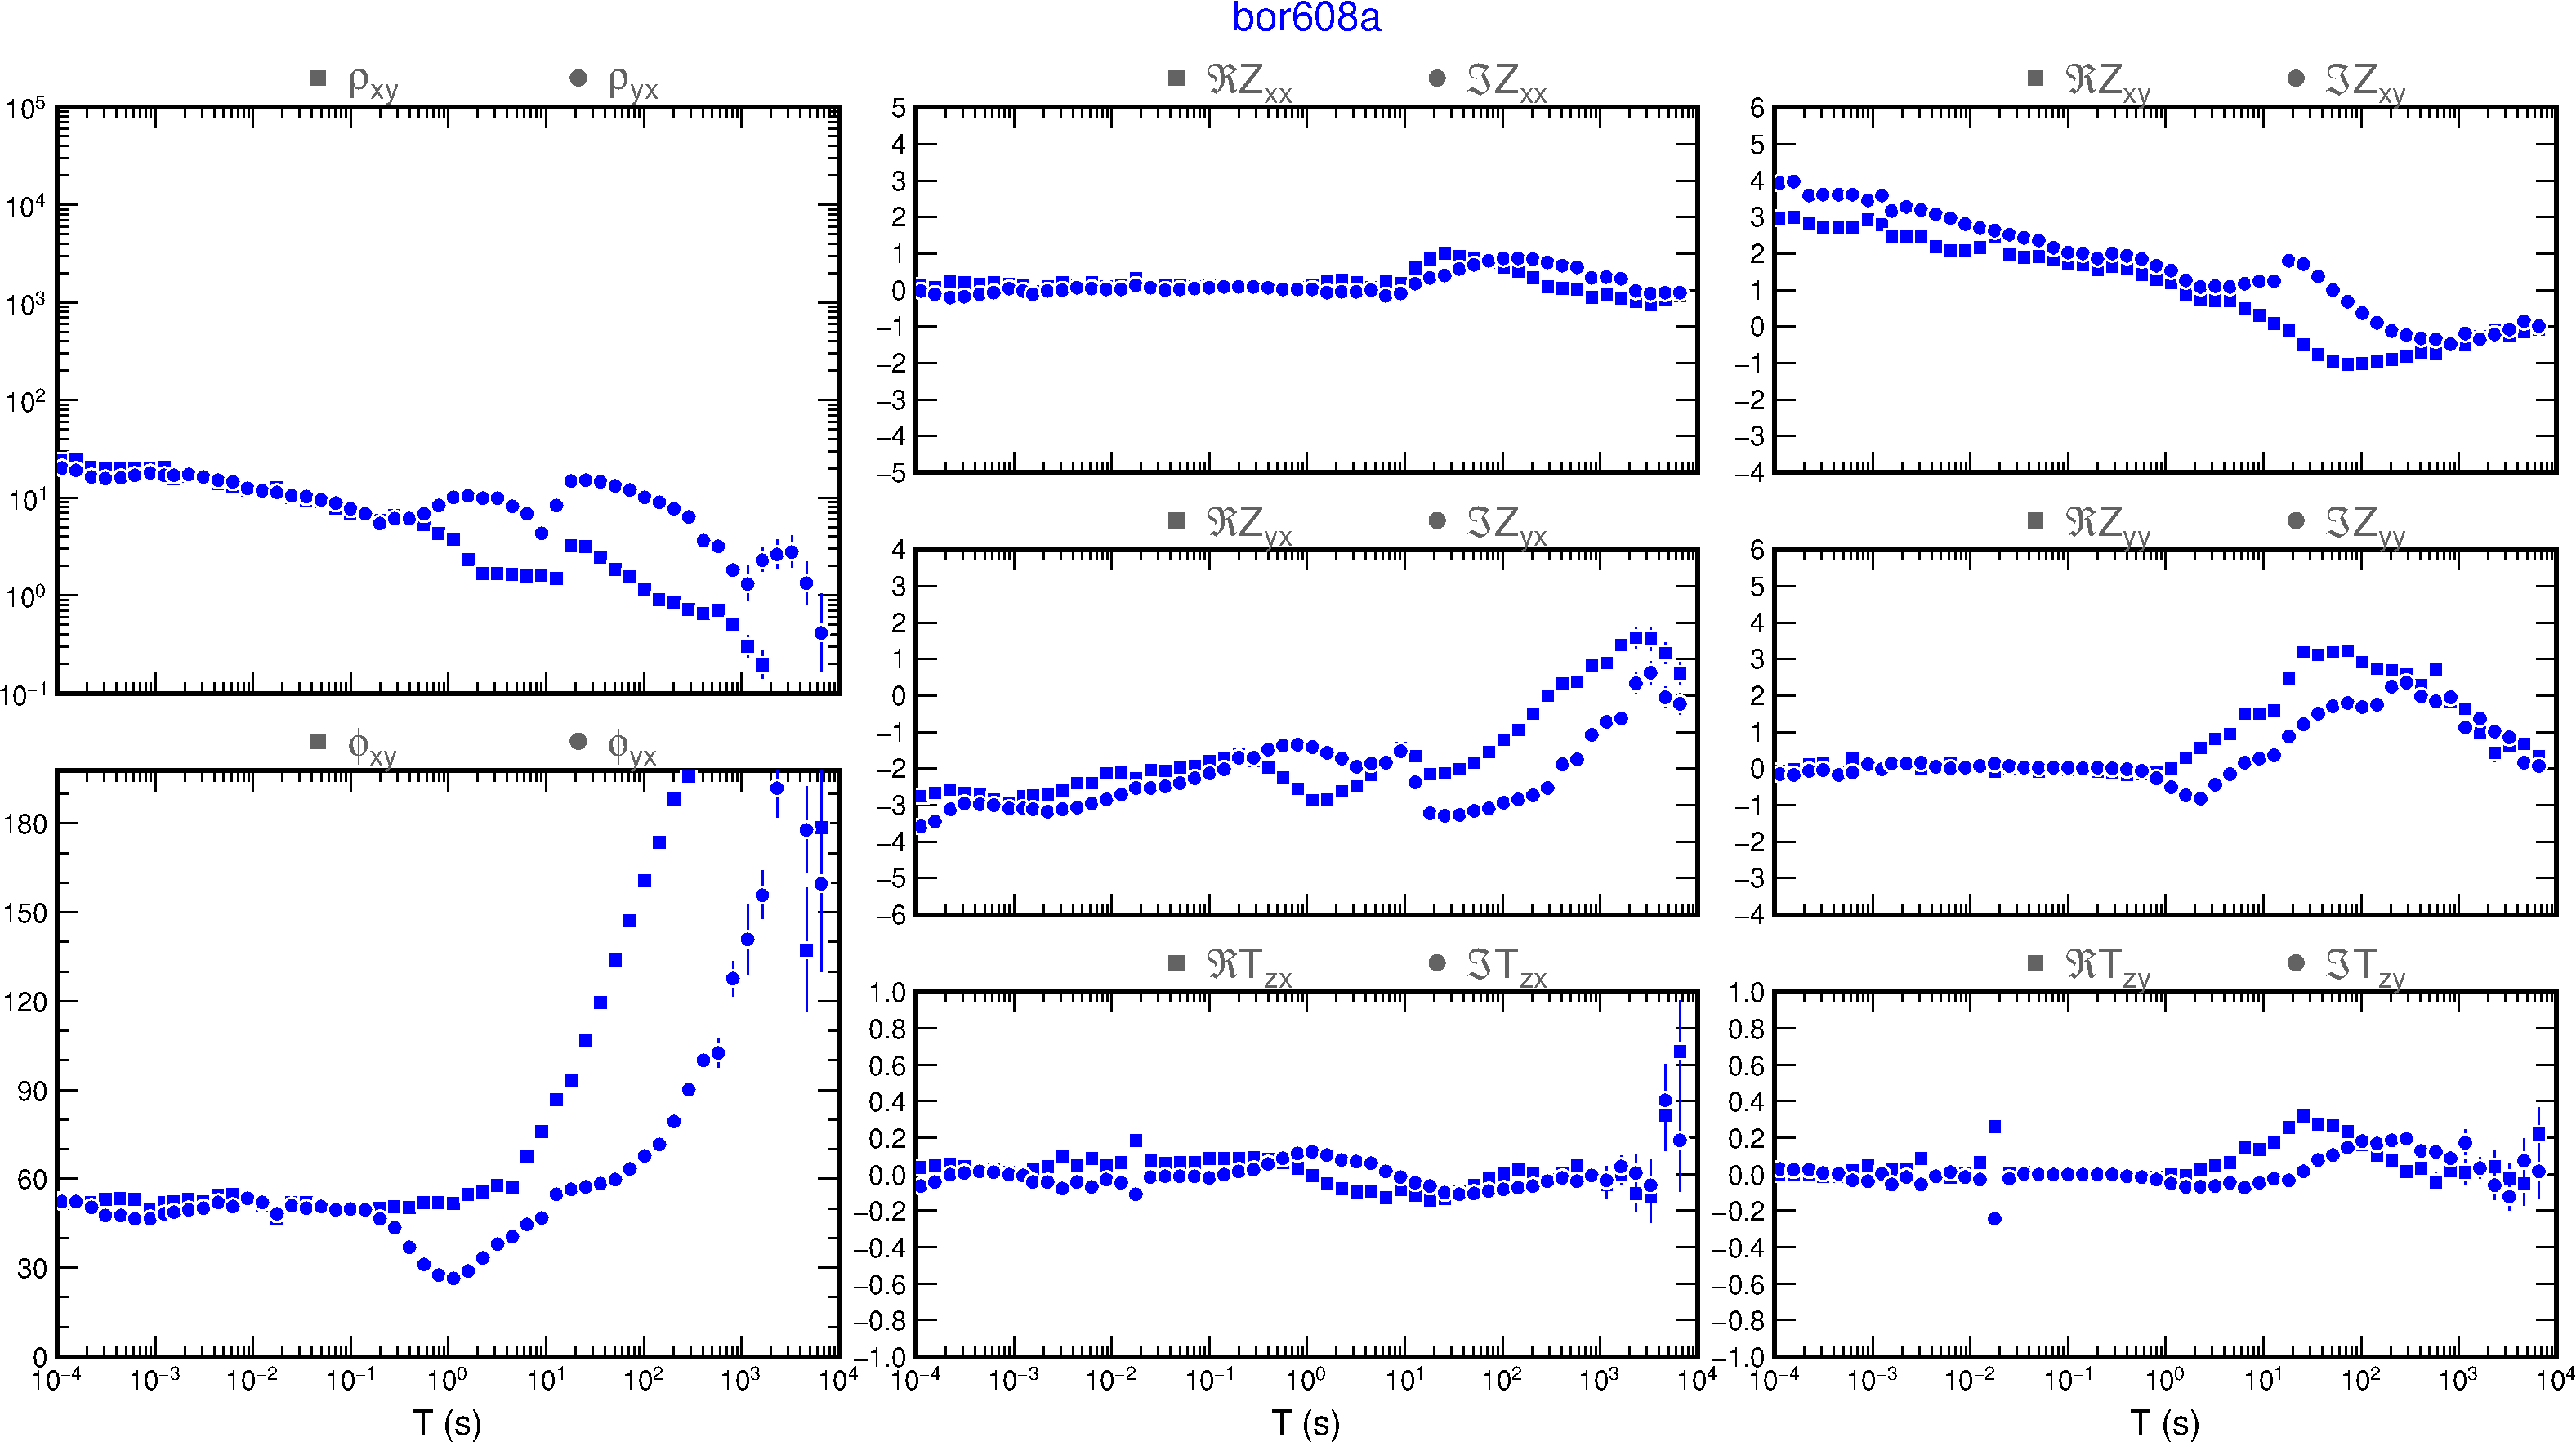
\includegraphics[width=16cm]{texto/figura/sites/M-bor608a.png}
            \end{center}
        \legend{\Fonte{\oautor.}}
    \end{figure}
    
    \begin{figure}[H]
        \caption{Manual -- bor608b}
            \begin{center}
                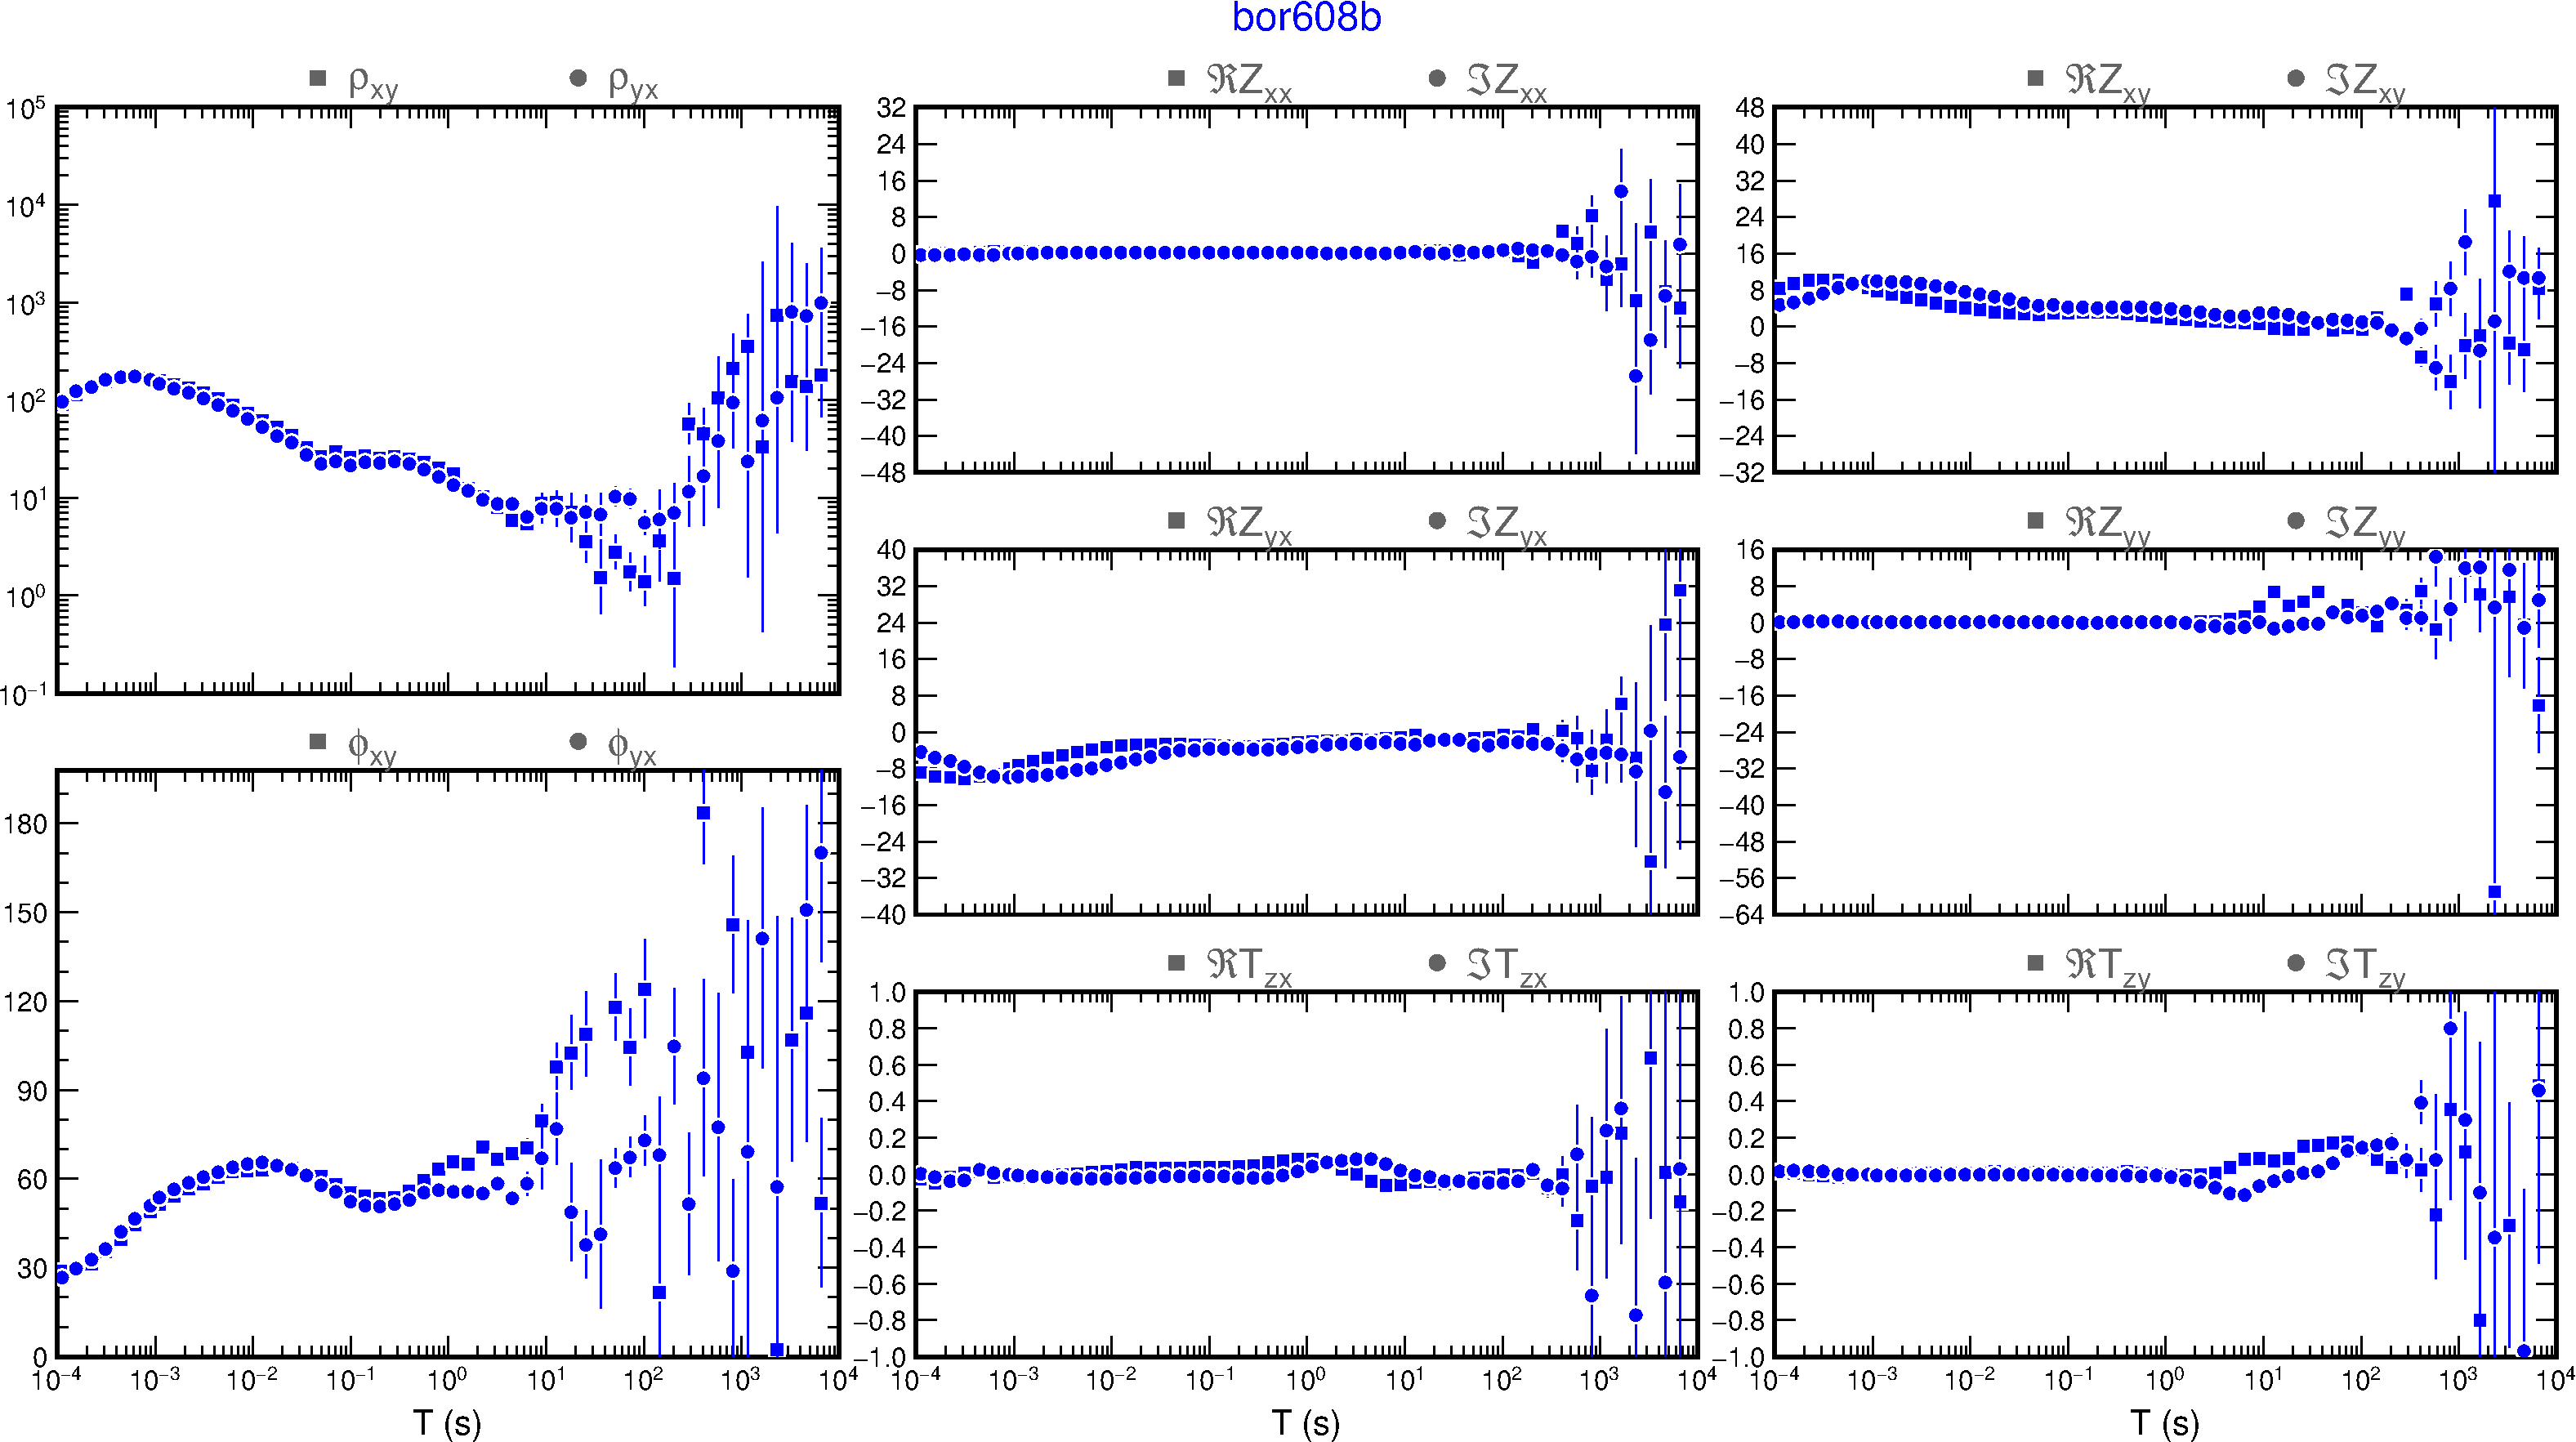
\includegraphics[width=16cm]{texto/figura/sites/M-bor608b.png}
            \end{center}
        \legend{\Fonte{\oautor.}}
    \end{figure}
    
    \begin{figure}[H]
        \caption{Manual -- bor608c}
            \begin{center}
                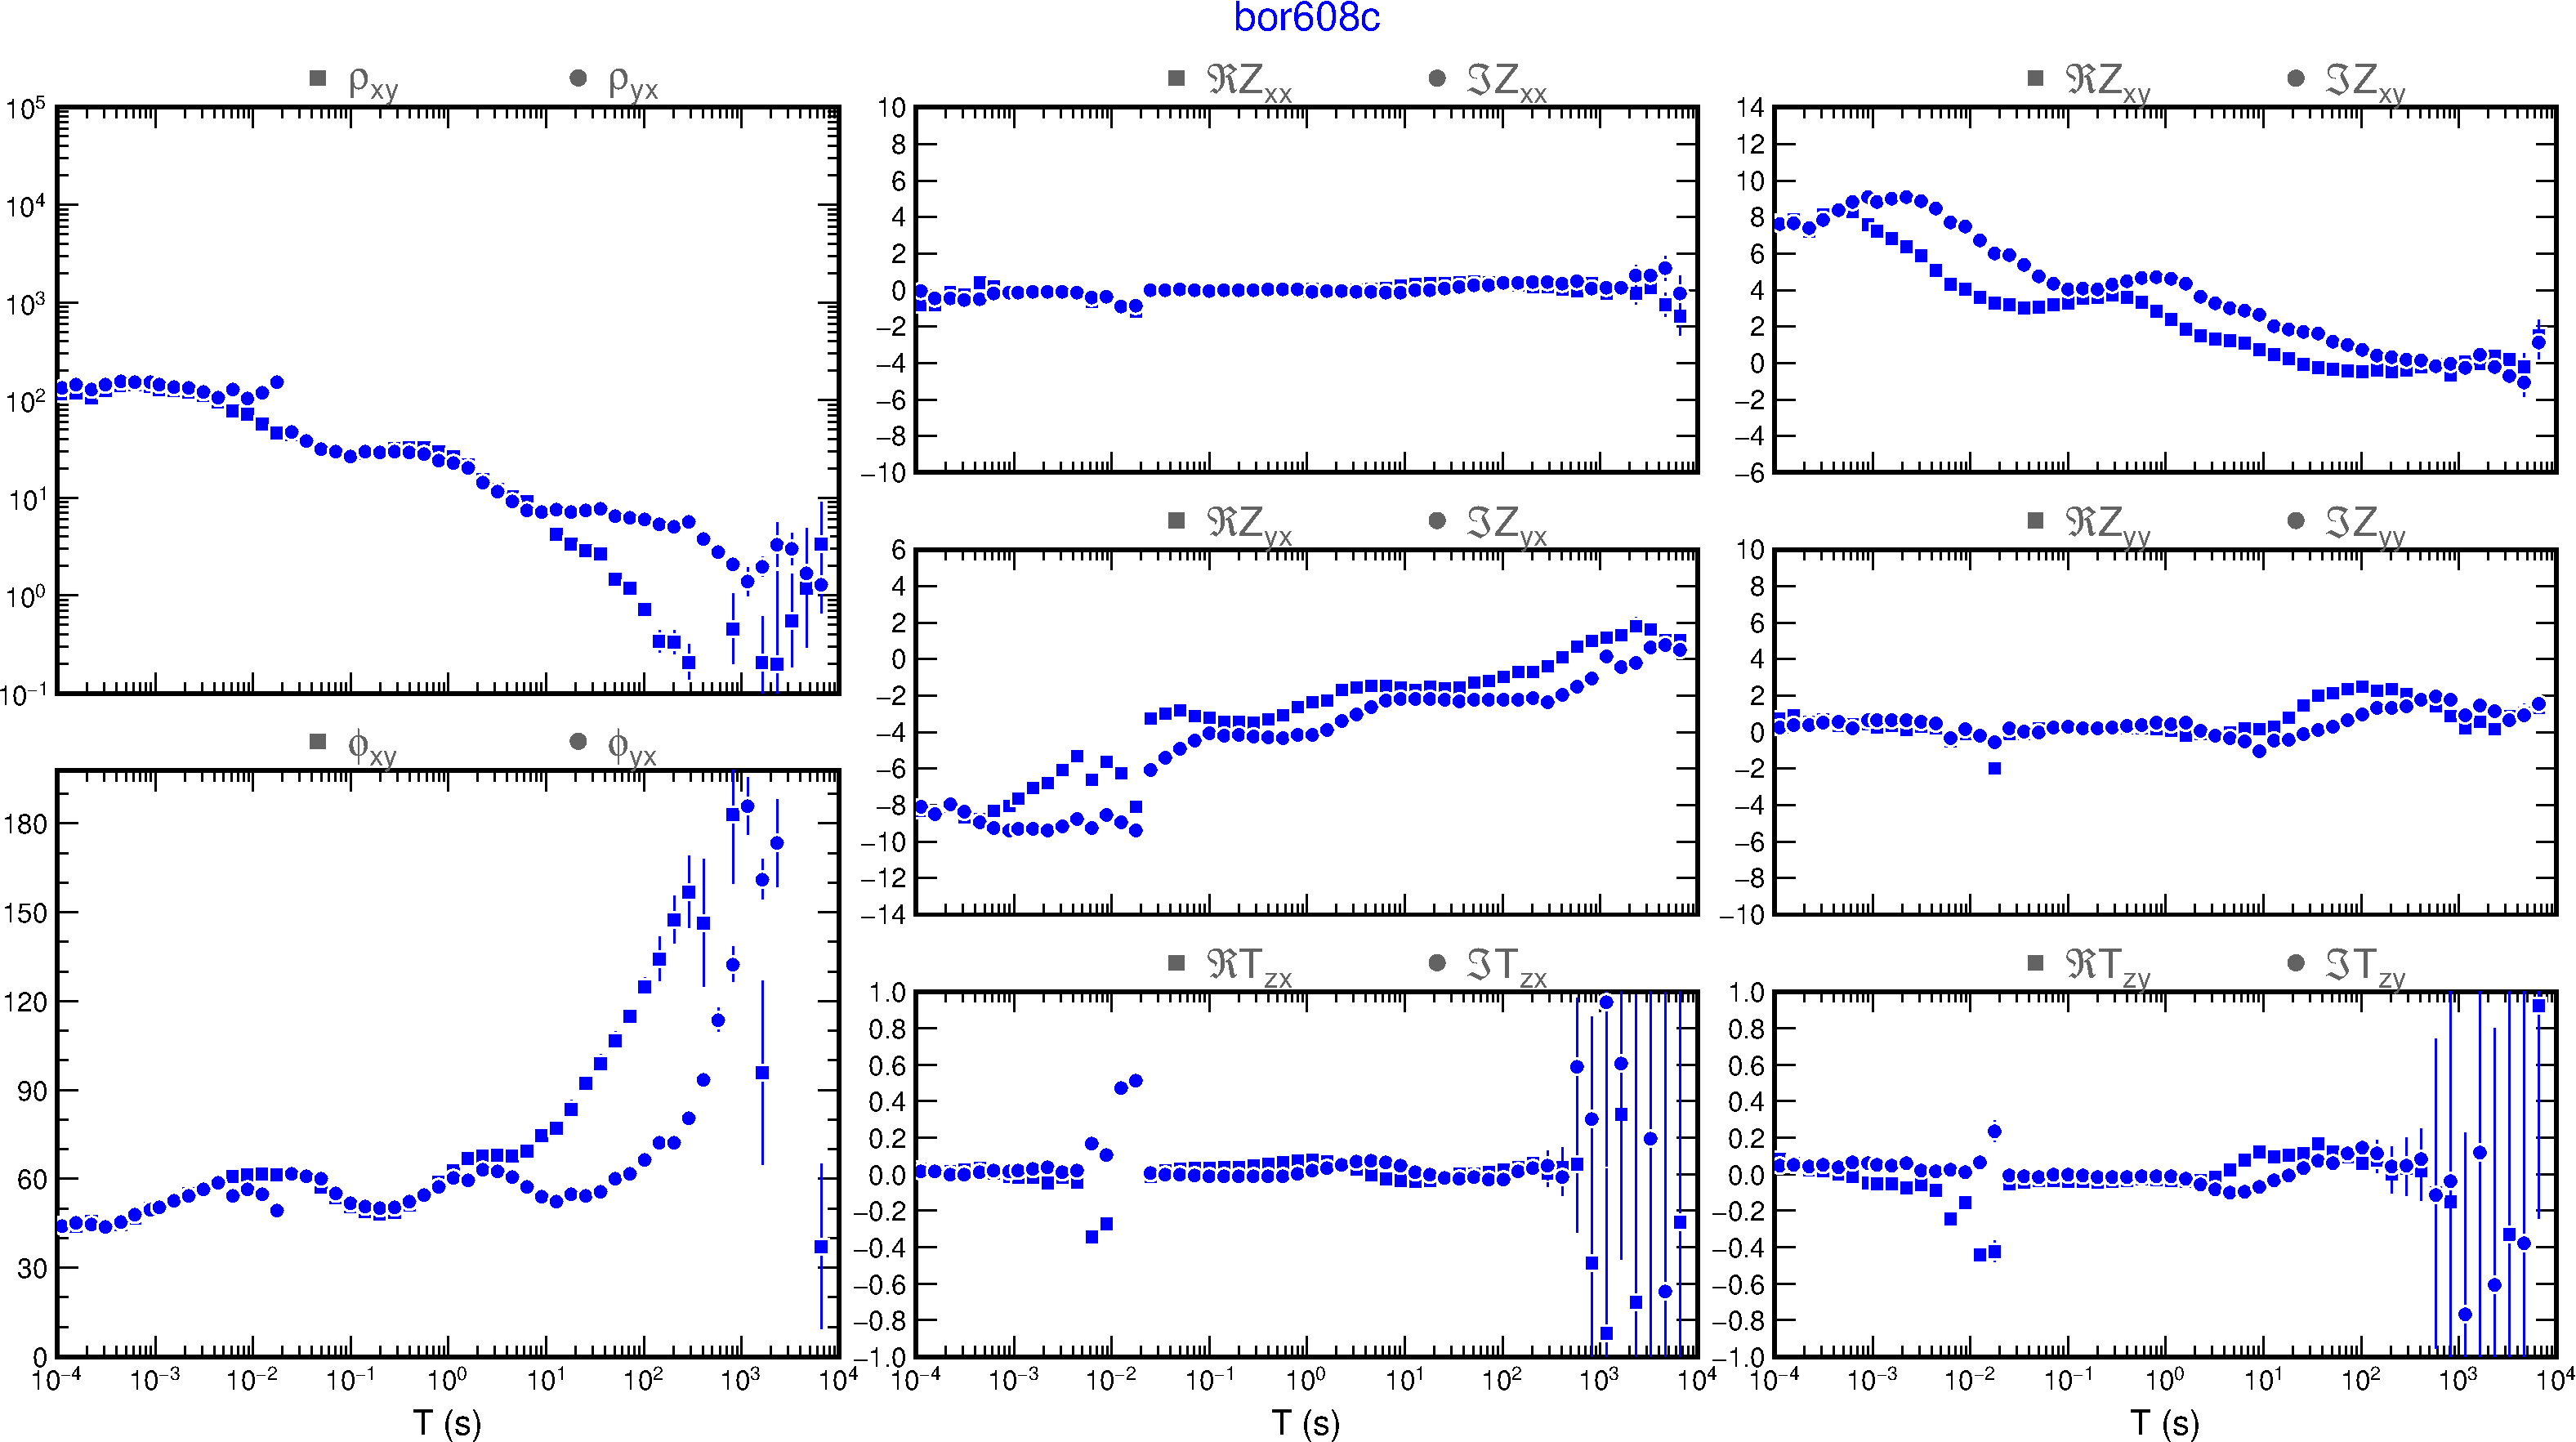
\includegraphics[width=16cm]{texto/figura/sites/M-bor608c.png}
            \end{center}
        \legend{\Fonte{\oautor.}}
    \end{figure}
    
\chapter{Pré-processamento Usando o PampaMT}

\begin{figure}[H]
        \caption{PampaMT -- bor603b}
            \begin{center}
                \includegraphics[width=15cm]{texto/figura/sites/P-bor603b.png}
            \end{center}
        \legend{\Fonte{\oautor.}}
    \end{figure}
    %\end{landscape}
    \begin{figure}[H]
        \caption{PampaMT -- bor604a}
            \begin{center}
                \includegraphics[width=15cm]{texto/figura/sites/P-bor604a.png}
            \end{center}
        \legend{\Fonte{\oautor.}}
    \end{figure}
    
    \begin{figure}[H]
        \caption{PampaMT -- bor604b}
            \begin{center}
                \includegraphics[width=16.5cm]{texto/figura/sites/P-bor604b.png}
            \end{center}
        \legend{\Fonte{\oautor.}}
    \end{figure}
    
    \begin{figure}[H]
        \caption{PampaMT -- bor605a}
            \begin{center}
                \includegraphics[width=16.5cm]{texto/figura/sites/P-bor605a.png}
            \end{center}
        \legend{\Fonte{\oautor.}}
    \end{figure}
    
    \begin{figure}[H]
        \caption{PampaMT -- bor605b}
            \begin{center}
                \includegraphics[width=16.5cm]{texto/figura/sites/P-bor605b.png}
            \end{center}
        \legend{\Fonte{\oautor.}}
    \end{figure}
    
    \begin{figure}[H]
        \caption{PampaMT -- bor606a}
            \begin{center}
                \includegraphics[width=16.5cm]{texto/figura/sites/P-bor606a.png}
            \end{center}
        \legend{\Fonte{\oautor.}}
    \end{figure}
    
    \begin{figure}[H]
        \caption{PampaMT -- bor606b}
            \begin{center}
                \includegraphics[width=16.5cm]{texto/figura/sites/P-bor606b.png}
            \end{center}
        \legend{\Fonte{\oautor.}}
    \end{figure}
    
    \begin{figure}[H]
        \caption{PampaMT -- bor607a}
            \begin{center}
                \includegraphics[width=16.5cm]{texto/figura/sites/P-bor607a.png}
            \end{center}
        \legend{\Fonte{\oautor.}}
    \end{figure}
    
    \begin{figure}[H]
        \caption{PampaMT -- bor607b}
            \begin{center}
                \includegraphics[width=16.5cm]{texto/figura/sites/P-bor607b.png}
            \end{center}
        \legend{\Fonte{\oautor.}}
    \end{figure}
    
    \begin{figure}[H]
        \caption{PampaMT -- bor608a}
            \begin{center}
                \includegraphics[width=16.5cm]{texto/figura/sites/P-bor608a.png}
            \end{center}
        \legend{\Fonte{\oautor.}}
    \end{figure}
    
    \begin{figure}[H]
        \caption{PampaMT -- bor608b}
            \begin{center}
                \includegraphics[width=16.5cm]{texto/figura/sites/P-bor608b.png}
            \end{center}
        \legend{\Fonte{\oautor.}}
    \end{figure}
    
    \begin{figure}[H]
        \caption{PampaMT -- bor608c}
            \begin{center}
                \includegraphics[width=16.5cm]{texto/figura/sites/P-bor608c.png}
            \end{center}
        \legend{\Fonte{\oautor.}}
    \end{figure}

%\chapter{Codigo fonte}
%    Conteudo do apendice A
% ==============================================================================


% ANEXO
% ==============================================================================
%\anexos                         % Inicia os anexos


% ==============================================================================

    
% INDICE
% ==============================================================================
% Para utilizar o indexamento automatico use no corpo do texto:
%   \index{palavra} 
%
%\printindex             % Imprime o indice
% ==============================================================================

\end{document}
